\documentclass[12pt]{article}
\usepackage{amsmath, amssymb, amsthm}
\usepackage{mathtools}
\usepackage{graphicx}
\usepackage{float}
\usepackage{hyperref}
\usepackage{xcolor}
\usepackage{listings}
\usepackage{geometry}
\usepackage{algorithm}
\usepackage{algpseudocode}
\usepackage{tikz}
\usepackage{longtable}
\usepackage{circuitikz}
\usepackage{comment}
\usepackage{MnSymbol}
\usepackage{physics}
\usepackage{booktabs}
\usepackage{subfig} % For \subfloat
\usepackage[section]{placeins}

\begin{document}

\begin{titlepage}
    \centering
    \vspace*{1.5cm}
    
    {\Huge\bfseries Group Quiz 2}\\[0.5cm]
    {\Large\bfseries Differential Equations and Transform Techniques (EE1060)}\\[1cm]
    {\Large\bfseries Detailed Analysis of Convolution for Continous Time Kernel}\\[1.5cm]
    
    \rule{0.8\textwidth}{0.4pt}\\[0.5cm]
    {\Large\bfseries Submitted By}\\[0.5cm]
    \rule{0.8\textwidth}{0.4pt}\\[0.5cm]
    
    \large
    Krishna Patil \hfill EE24BTECH11036\\[0.2cm]
    Agamjot Singh \hfill EE24BTECH11002\\[0.2cm]
    Kollaru Suraj \hfill EE24BTECH11033\\[0.2cm]
    Dwanith M Doddahundi \hfill EE24BTECH11016\\[0.2cm]
    Swaraj Sharma Durgi \hfill EE24BTECH11018\\[0.2cm]
    Nevanath Vasu \hfill EE24BTECH11046\\[1.5cm]
    
\end{titlepage}


\tableofcontents
\newpage

\section{Problem Statement}
\begin{enumerate}
\item Compute the convolution of a given signal $f(t)$ with a rectangular kernel $h(t)$, analytically. The rectangular kernel is defined as:

\begin{equation}
h(t) =
\begin{cases}
1, & \text{for } -T \leq t \leq T \\
0, & \text{otherwise}
\end{cases}
\end{equation}

Derive the convolution expression $y(t) = (f * h)(t)$ in terms of known functions, and analyze the system's behavior for various values of the kernel duration $T$ and the input signal $f(t)$. Additionally, investigate the following scenarios:

\begin{enumerate}
\item Modify the kernel to only consider the part of the kernel for $t > 0$. How does this affect the convolution result?

\item Shift the kernel by a time $\tau_0$. Analyze how the shift impacts the convolution output and discuss the significance of this shift in the context of time-delayed systems.
\end{enumerate}

You are free to choose the form of the input signal $f(t)$, but make sure it is well-defined and appropriate for convolution. A step or sinusoidal signal would work well for this analysis.
\end{enumerate}

\section{Step Signal as $f(t)$}
For this analysis, we choose the \textbf{unit step function} as the input signal:

\begin{equation}
f(t) = u(t) = 
\begin{cases} 
1, & t \geq 0 \\
0, & t < 0 
\end{cases}
\end{equation}

\subsubsection{Interpretation:}
\begin{itemize}
    \item The output \( y(t) \) represents how the shape of \( f(t) \) is modified by \( h(t) \).
    \item The rectangular kernel \( h(t) \) acts as a moving average filter.
\end{itemize}

\subsection{Solution Using Step Function}

\subsubsection{Standard Convolution \( y(t) = (f * h)(t) \)}

Given:
\begin{itemize}
    \item \( f(t) = u(t) \) (step function)
    \item \( h(t) \) is a rectangular pulse centered at \( t = 0 \) with width \( 2T \).
\end{itemize}

The convolution integral is evaluated in three regions:

\begin{enumerate}
    \item \textbf{For \( t < -T \):}
    \begin{itemize}
        \item The kernel \( h(t - \tau) \) and \( u(\tau) \) do not overlap.
        \item Thus:
    \end{itemize}
    
    \begin{align}
        y(t) &= \int_{-\infty}^{\infty} u(\tau) h(t - \tau) \, d\tau \\
        &= \int_{0}^{\infty} 1 \cdot h(t - \tau) \, d\tau \\
        &= 0 \quad \text{(No overlap when $t < -T$)}
    \end{align}
    
    \item \textbf{For \( -T \leq t \leq T \):}
    \begin{itemize}
        \item The kernel partially overlaps \( u(\tau) \) from \( \tau = 0 \) to \( \tau = t + T \).
    \end{itemize}
    
    \begin{align}
        y(t) &= \int_{-\infty}^{\infty} u(\tau) h(t - \tau) \, d\tau \\
        &= \int_{0}^{\infty} 1 \cdot h(t - \tau) \, d\tau \\
        &= \int_{0}^{t+T} 1 \cdot 1 \, d\tau \quad \text{(Since $h(t-\tau)=1$ when $-T \leq t-\tau \leq T$)} \\
        &= [{\tau}]_{0}^{t+T} \\
        &= t + T
    \end{align}
    
    \item \textbf{For \( t > T \):}
    \begin{itemize}
        \item The kernel fully overlaps \( u(\tau) \) over a width of \( 2T \).
    \end{itemize}
    
    \begin{align}
        y(t) &= \int_{-\infty}^{\infty} u(\tau) h(t - \tau) \, d\tau \\
        &= \int_{0}^{\infty} 1 \cdot h(t - \tau) \, d\tau \\
        &= \int_{t-T}^{t+T} 1 \, d\tau \quad \text{(Since $h(t-\tau)=1$ when $t-T \leq \tau \leq t+T$)} \\
        &= [{\tau}]_{t-T}^{t+T} \\
        &= (t+T) - (t-T) \\
        &= 2T
    \end{align}
\end{enumerate}

\textbf{Final Result:}
\begin{equation}
y(t) = 
\begin{cases} 
0, & t < -T \\
t + T, & -T \leq t \leq T \\
2T, & t > T 
\end{cases}
\end{equation}

\subsubsection{Behavior Analysis:}
\begin{itemize}
    \item The output is zero before \( t = -T \).
    \item A linear ramp occurs from \( t = -T \) to \( t = T \).
    \item The output saturates at \( 2T \) for \( t > T \).
    \item A larger \( T \) results in a wider ramp and higher saturation value.
\end{itemize}
Here is plot showing the results
\begin{figure}[H]
    \centering
    \includegraphics[width=0.8\linewidth]{codes/codes_step/plotsstep/case1step.png}
    \label{fig:enter-label}
\end{figure}
\subsubsection{Modified Kernel (Only \( t > 0 \)) (Part a)}

The modified kernel is:
\begin{equation}
h_{mod}(t) = 
\begin{cases} 
1, & 0 \leq t \leq T \\
0, & \text{otherwise}
\end{cases}
\end{equation}

\textbf{Convolution Analysis:}

\begin{enumerate}
    \item \textbf{For \( t < 0 \):}
    \begin{align}
        y(t) &= \int_{-\infty}^{\infty} u(\tau) h_{mod}(t - \tau) \, d\tau \\
        &= 0 \quad \text{(No overlap when $t < 0$)}
    \end{align}
    
    \item \textbf{For \( 0 \leq t \leq T \):}
    \begin{align}
        y(t) &= \int_{-\infty}^{\infty} u(\tau) h_{mod}(t - \tau) \, d\tau \\
        &= \int_{0}^{t} 1 \cdot 1 \, d\tau \quad \text{(Overlap from $\tau = 0$ to $\tau = t$)} \\
        &= [{\tau}]_{0}^{t} \\
        &= t
    \end{align}
    
    \item \textbf{For \( t > T \):}
    \begin{align}
        y(t) &= \int_{-\infty}^{\infty} u(\tau) h_{mod}(t - \tau) \, d\tau \\
        &= \int_{t-T}^{t} 1 \cdot 1 \, d\tau \quad \text{(Full overlap from $\tau = t-T$ to $\tau = t$)} \\
        &= [{\tau}]_{t-T}^{t} \\
        &= t - (t-T) \\
        &= T
    \end{align}
\end{enumerate}

\textbf{Result:}
\begin{equation}
y(t) = 
\begin{cases} 
0, & t < 0 \\
t, & 0 \leq t \leq T \\
T, & t > T 
\end{cases}
\end{equation}
Here is a plot showing the results
\begin{figure}[H]
    \centering
    \includegraphics[width=0.8\linewidth]{codes/codes_step/plotsstep/case2step.png}
    \caption{Modified kernel}
    \label{fig:enter-label}
\end{figure}
\subsubsection{Comparison with Original Kernel:}
\begin{itemize}
    \item The response is now \textbf{causal} (output depends only on past/current inputs).
    \item The ramp is shorter (from \( 0 \) to \( T \)) compared to the original (\( -T \) to \( T \)).
    \item The steady-state value is \( T \) instead of \( 2T \).
\end{itemize}

\subsubsection{Shifted Kernel by \( \tau_0 \) (Part b)}

The shifted kernel is:
\begin{equation}
h_{shift}(t) = 
\begin{cases} 
1, & -T + \tau_0 \leq t \leq T + \tau_0 \\
0, & \text{otherwise}
\end{cases}
\end{equation}

Applying the time-shift property of convolution:
\begin{align}
f(t) * h(t-\tau_0) = (f(t) * h(t))_{t \rightarrow t-\tau_0}
\end{align}

The convolution output is simply the original \( y(t) \) delayed by \( \tau_0 \):

\begin{equation}
y_{shift}(t) = y(t - \tau_0) = 
\begin{cases} 
0, & t < -T + \tau_0 \\
(t - \tau_0) + T, & -T + \tau_0 \leq t \leq T + \tau_0 \\
2T, & t > T + \tau_0 
\end{cases}
\end{equation}
\begin{figure}[H]
    \centering
    \includegraphics[width=0.8\linewidth]{codes/codes_step/plotsstep/case3step.png}
    \caption{shifted kernel}
    \label{fig:enter-label}
\end{figure}

\subsubsection{Significance in Time-Delayed Systems:}
\begin{itemize}
    \item The shift \( \tau_0 \) introduces a \textbf{time delay} in the system's response.
    \item For \( \tau_0 > 0 \), the response is delayed (system responds later).
    \item For \( \tau_0 < 0 \), the response is advanced (system responds earlier).
    \item Important in control systems, signal processing, and communications where delays affect stability and synchronization.
\end{itemize}

\subsection{Conclusion}

\begin{itemize}
    \item The convolution of a step function with a rectangular kernel produces a \textbf{piecewise linear} output.
    \item Modifying the kernel to be \textbf{causal} changes the response to depend only on past inputs.
    \item Shifting the kernel introduces a \textbf{time delay}, which is crucial in real-world systems.
    \item The kernel width \( T \) directly affects the steady-state value and transition time of the output.
\end{itemize}

This analysis demonstrates how different kernel modifications affect signal processing outcomes and provides insight into the behavior of linear time-invariant systems.
\subsubsection{Comparision of all cases}
\begin{figure}[H]
    \centering
    \includegraphics[width=0.8\linewidth]{codes/codes_step/plotsstep/comparsionof123.png}
    \caption{Comparision of all cases}
    \label{fig:enter-label}
\end{figure}

\section*{1. Problem Statement}

\subsection*{1.1 Convolution with a Rectangular Kernel}
Compute the convolution of a given signal \( f(t) \) with a rectangular kernel \( h(t) \), analytically. The rectangular kernel is defined as:

\begin{equation}
h(t) = 
\begin{cases} 
1, & \text{for } -T \leq t \leq T \\
0, & \text{otherwise}
\end{cases}
\end{equation}

Derive the convolution expression \( y(t) = (f * h)(t) \) in terms of known functions, and analyze the system's behavior for various values of the kernel duration \( T \) and the input signal \( f(t) \).

Additionally, investigate the following scenarios:

\begin{enumerate}
    \item[(a)] Modify the kernel to only consider the part for \( t > 0 \). How does this affect the convolution result?
    \item[(b)] Shift the kernel by a time \( \tau_0 \). Analyze how the shift impacts the convolution output and discuss its significance in time-delayed systems.
\end{enumerate}

\textbf{Choice of Input Signal:}\\
For this analysis, we choose the \textbf{unit step function} as the input signal:

\begin{equation}
f(t) = u(t) = 
\begin{cases} 
1, & t \geq 0 \\
0, & t < 0 
\end{cases}
\end{equation}

\section*{2. Convolution Basics}

The convolution of two signals \( f(t) \) and \( h(t) \) is defined as:

\begin{equation}
y(t) = (f * h)(t) = \int_{-\infty}^{\infty} f(\tau) h(t - \tau) \, d\tau
\end{equation}

\subsection*{Interpretation:}
\begin{itemize}
    \item The output \( y(t) \) represents how the shape of \( f(t) \) is modified by \( h(t) \).
    \item The rectangular kernel \( h(t) \) acts as a moving average filter.
\end{itemize}

\section*{3. Solution Using Step Function}

\subsection*{3.1 Standard Convolution \( y(t) = (f * h)(t) \)}

Given:
\begin{itemize}
    \item \( f(t) = u(t) \) (step function)
    \item \( h(t) \) is a rectangular pulse centered at \( t = 0 \) with width \( 2T \).
\end{itemize}

The convolution integral is evaluated in three regions:

\begin{enumerate}
    \item \textbf{For \( t < -T \):}
    \begin{itemize}
        \item The kernel \( h(t - \tau) \) and \( u(\tau) \) do not overlap.
        \item Thus:
    \end{itemize}
    
    \begin{align}
        y(t) &= \int_{-\infty}^{\infty} u(\tau) h(t - \tau) \, d\tau \\
        &= \int_{0}^{\infty} 1 \cdot h(t - \tau) \, d\tau \\
        &= 0 \quad \text{(No overlap when $t < -T$)}
    \end{align}
    
    \item \textbf{For \( -T \leq t \leq T \):}
    \begin{itemize}
        \item The kernel partially overlaps \( u(\tau) \) from \( \tau = 0 \) to \( \tau = t + T \).
    \end{itemize}
    
    \begin{align}
        y(t) &= \int_{-\infty}^{\infty} u(\tau) h(t - \tau) \, d\tau \\
        &= \int_{0}^{\infty} 1 \cdot h(t - \tau) \, d\tau \\
        &= \int_{0}^{t+T} 1 \cdot 1 \, d\tau \quad \text{(Since $h(t-\tau)=1$ when $-T \leq t-\tau \leq T$)} \\
        &= [{\tau}]_{0}^{t+T} \\
        &= t + T
    \end{align}
    
    \item \textbf{For \( t > T \):}
    \begin{itemize}
        \item The kernel fully overlaps \( u(\tau) \) over a width of \( 2T \).
    \end{itemize}
    
    \begin{align}
        y(t) &= \int_{-\infty}^{\infty} u(\tau) h(t - \tau) \, d\tau \\
        &= \int_{0}^{\infty} 1 \cdot h(t - \tau) \, d\tau \\
        &= \int_{t-T}^{t+T} 1 \, d\tau \quad \text{(Since $h(t-\tau)=1$ when $t-T \leq \tau \leq t+T$)} \\
        &= [{\tau}]_{t-T}^{t+T} \\
        &= (t+T) - (t-T) \\
        &= 2T
    \end{align}
\end{enumerate}

\textbf{Final Result:}
\begin{equation}
y(t) = 
\begin{cases} 
0, & t < -T \\
t + T, & -T \leq t \leq T \\
2T, & t > T 
\end{cases}
\end{equation}

\subsection*{Behavior Analysis:}
\begin{itemize}
    \item The output is zero before \( t = -T \).
    \item A linear ramp occurs from \( t = -T \) to \( t = T \).
    \item The output saturates at \( 2T \) for \( t > T \).
    \item A larger \( T \) results in a wider ramp and higher saturation value.
\end{itemize}
Here is plot showing the results
\begin{figure}[H]
    \centering
    \includegraphics[width=0.8\linewidth]{plotsstep/case1step.png}
    \label{fig:enter-label}
\end{figure}
\subsection*{3.2 Modified Kernel (Only \( t > 0 \)) (Part a)}

The modified kernel is:
\begin{equation}
h_{mod}(t) = 
\begin{cases} 
1, & 0 \leq t \leq T \\
0, & \text{otherwise}
\end{cases}
\end{equation}

\textbf{Convolution Analysis:}

\begin{enumerate}
    \item \textbf{For \( t < 0 \):}
    \begin{align}
        y(t) &= \int_{-\infty}^{\infty} u(\tau) h_{mod}(t - \tau) \, d\tau \\
        &= 0 \quad \text{(No overlap when $t < 0$)}
    \end{align}
    
    \item \textbf{For \( 0 \leq t \leq T \):}
    \begin{align}
        y(t) &= \int_{-\infty}^{\infty} u(\tau) h_{mod}(t - \tau) \, d\tau \\
        &= \int_{0}^{t} 1 \cdot 1 \, d\tau \quad \text{(Overlap from $\tau = 0$ to $\tau = t$)} \\
        &= [{\tau}]_{0}^{t} \\
        &= t
    \end{align}
    
    \item \textbf{For \( t > T \):}
    \begin{align}
        y(t) &= \int_{-\infty}^{\infty} u(\tau) h_{mod}(t - \tau) \, d\tau \\
        &= \int_{t-T}^{t} 1 \cdot 1 \, d\tau \quad \text{(Full overlap from $\tau = t-T$ to $\tau = t$)} \\
        &= [{\tau}]_{t-T}^{t} \\
        &= t - (t-T) \\
        &= T
    \end{align}
\end{enumerate}

\textbf{Result:}
\begin{equation}
y(t) = 
\begin{cases} 
0, & t < 0 \\
t, & 0 \leq t \leq T \\
T, & t > T 
\end{cases}
\end{equation}
Here is a plot showing the results
\begin{figure}[H]
    \centering
    \includegraphics[width=0.8\linewidth]{plotsstep/case2step.png}
    \caption{Modified kernel}
    \label{fig:enter-label}
\end{figure}
\subsection*{Comparison with Original Kernel:}
\begin{itemize}
    \item The response is now \textbf{causal} (output depends only on past/current inputs).
    \item The ramp is shorter (from \( 0 \) to \( T \)) compared to the original (\( -T \) to \( T \)).
    \item The steady-state value is \( T \) instead of \( 2T \).
\end{itemize}

\subsection*{3.3 Shifted Kernel by \( \tau_0 \) (Part b)}

The shifted kernel is:
\begin{equation}
h_{shift}(t) = 
\begin{cases} 
1, & -T + \tau_0 \leq t \leq T + \tau_0 \\
0, & \text{otherwise}
\end{cases}
\end{equation}

Applying the time-shift property of convolution:
\begin{align}
f(t) * h(t-\tau_0) = (f(t) * h(t))_{t \rightarrow t-\tau_0}
\end{align}

The convolution output is simply the original \( y(t) \) delayed by \( \tau_0 \):

\begin{equation}
y_{shift}(t) = y(t - \tau_0) = 
\begin{cases} 
0, & t < -T + \tau_0 \\
(t - \tau_0) + T, & -T + \tau_0 \leq t \leq T + \tau_0 \\
2T, & t > T + \tau_0 
\end{cases}
\end{equation}
\begin{figure}[H]
    \centering
    \includegraphics[width=0.8\linewidth]{plotsstep/case3step.png}
    \caption{shifted kernel}
    \label{fig:enter-label}
\end{figure}
\subsection*{Significance in Time-Delayed Systems:}
\begin{itemize}
    \item The shift \( \tau_0 \) introduces a \textbf{time delay} in the system's response.
    \item For \( \tau_0 > 0 \), the response is delayed (system responds later).
    \item For \( \tau_0 < 0 \), the response is advanced (system responds earlier).
    \item Important in control systems, signal processing, and communications where delays affect stability and synchronization.
\end{itemize}

\section*{4. Conclusion}

\begin{itemize}
    \item The convolution of a step function with a rectangular kernel produces a \textbf{piecewise linear} output.
    \item Modifying the kernel to be \textbf{causal} changes the response to depend only on past inputs.
    \item Shifting the kernel introduces a \textbf{time delay}, which is crucial in real-world systems.
    \item The kernel width \( T \) directly affects the steady-state value and transition time of the output.
\end{itemize}

This analysis demonstrates how different kernel modifications affect signal processing outcomes and provides insight into the behavior of linear time-invariant systems.
\subsection*{Comparision of all cases}
\begin{figure}[H]
    \centering
    \includegraphics[width=0.8\linewidth]{plotsstep/comparsionof123.png}
    \caption{Comparision of all cases}
    \label{fig:enter-label}
\end{figure}

\section{Sinusoidal $f(t)$ with normal box kernel}
This report analyzes how the convolution of a sinusoidal signal with a rectangular kernel depends on various parameters. We consider the input signal $f(t) = A\sin(\omega t + \phi)$ and the rectangular kernel $h(t) = 1$ for $-T \leq t \leq T$ and 0 elsewhere.

\subsection{Analytical Solution}
The convolution of $f(t)$ with $h(t)$ is given by:
\begin{equation}
y(t) = (f * h)(t) = \int_{-\infty}^{\infty} f(\tau)h(t-\tau)d\tau
\end{equation}

For our specific functions, this simplifies to:
\begin{align}
y(t) &= \int_{t-T}^{t+T} A\sin(\omega\tau + \phi)d\tau\\
&= \frac{A}{\omega}[\cos(\omega(t-T) + \phi) - \cos(\omega(t+T) + \phi)]\\
&= \frac{2A}{\omega}\sin(\omega T)\sin(\omega t + \phi)
\end{align}

\subsection{Parameter Dependencies}

\subsubsection{Effect of Input Signal Amplitude}
The amplitude $A$ of the input signal linearly scales the output amplitude. As shown in Figure \ref{fig:amplitude}, the convolution output preserves this linear relationship, with the output amplitude being $\frac{2A}{\omega}\sin(\omega T)$ times the input amplitude.

\begin{figure}[H]
    \centering
    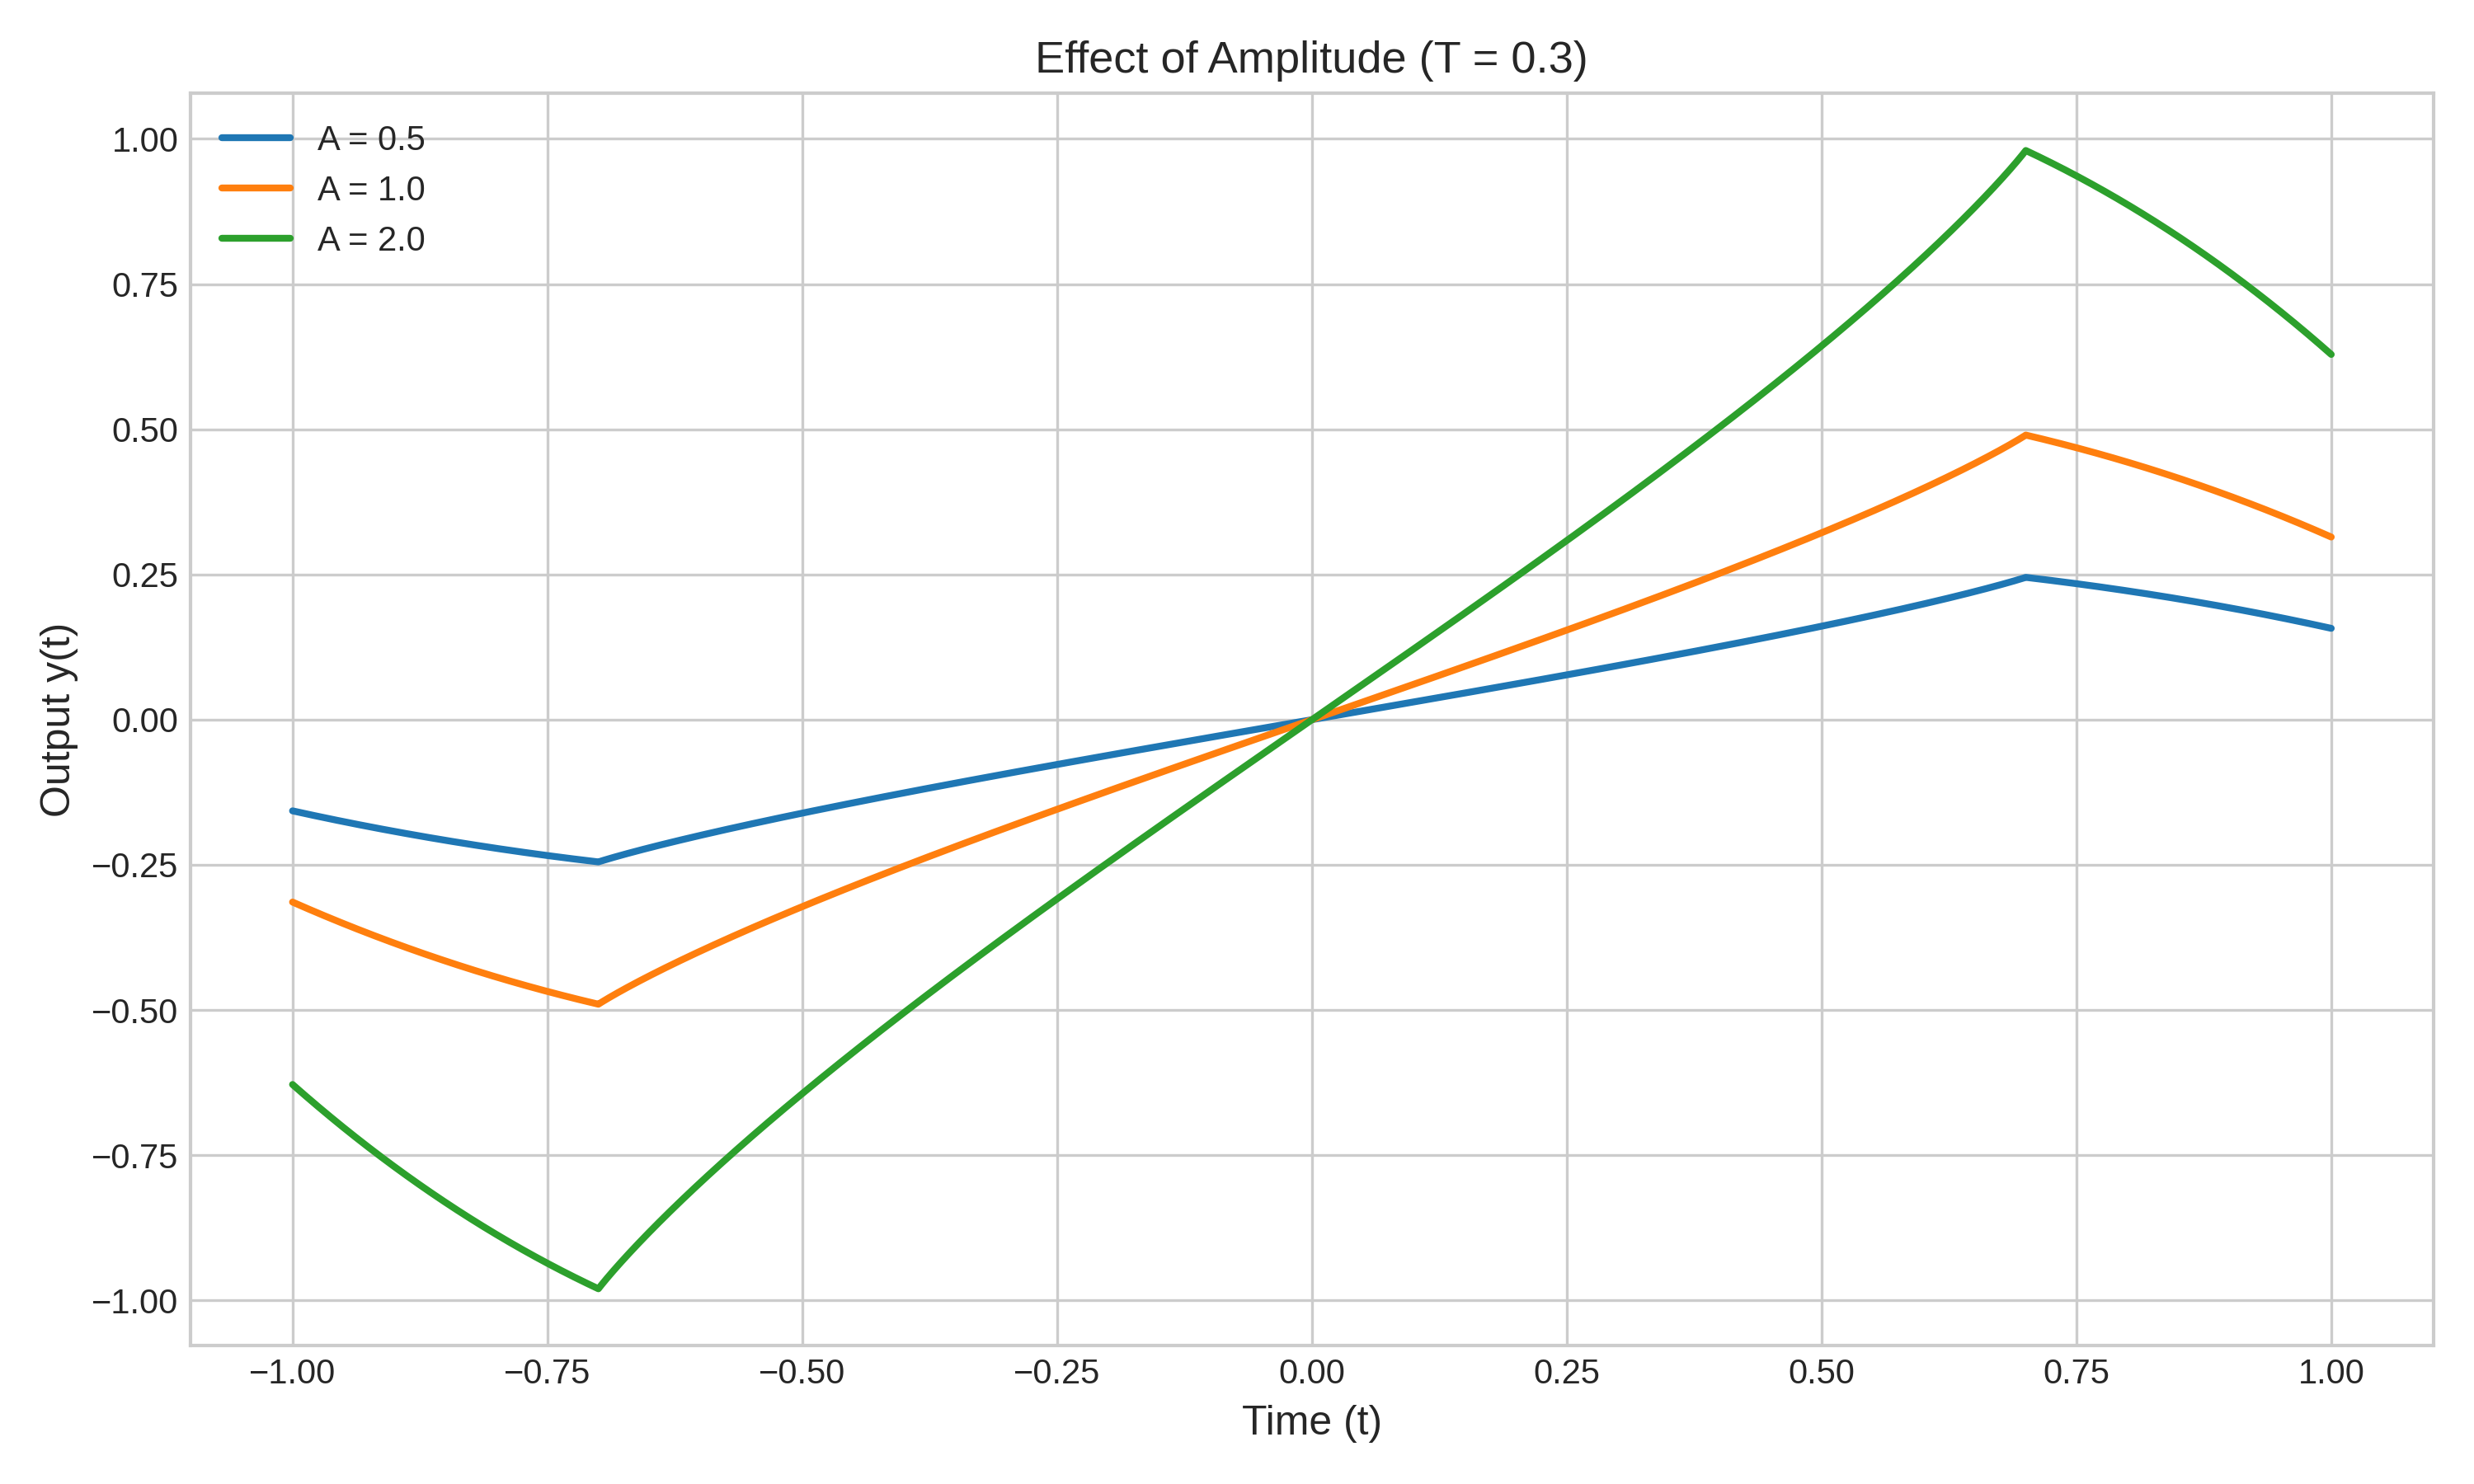
\includegraphics[width=0.8\textwidth]{codes/codes_sin_1_and_arcsin/figures/amplitude_effect.png}
    \caption{Effect of varying input signal amplitude on convolution output.}
    \label{fig:amplitude}
\end{figure}

\subsubsection{Effect of Input Signal Frequency}
The frequency $\omega$ affects the convolution in two ways:
\begin{enumerate}
    \item It determines the oscillation rate of the output signal
    \item It scales the output amplitude through the factor $\frac{2\sin(\omega T)}{\omega}$
\end{enumerate}

Higher frequencies generally result in smaller amplitudes due to the $\frac{1}{\omega}$ in the amplitude factor, as demonstrated in Figure \ref{fig:frequency}.

\begin{figure}[H]
    \centering
    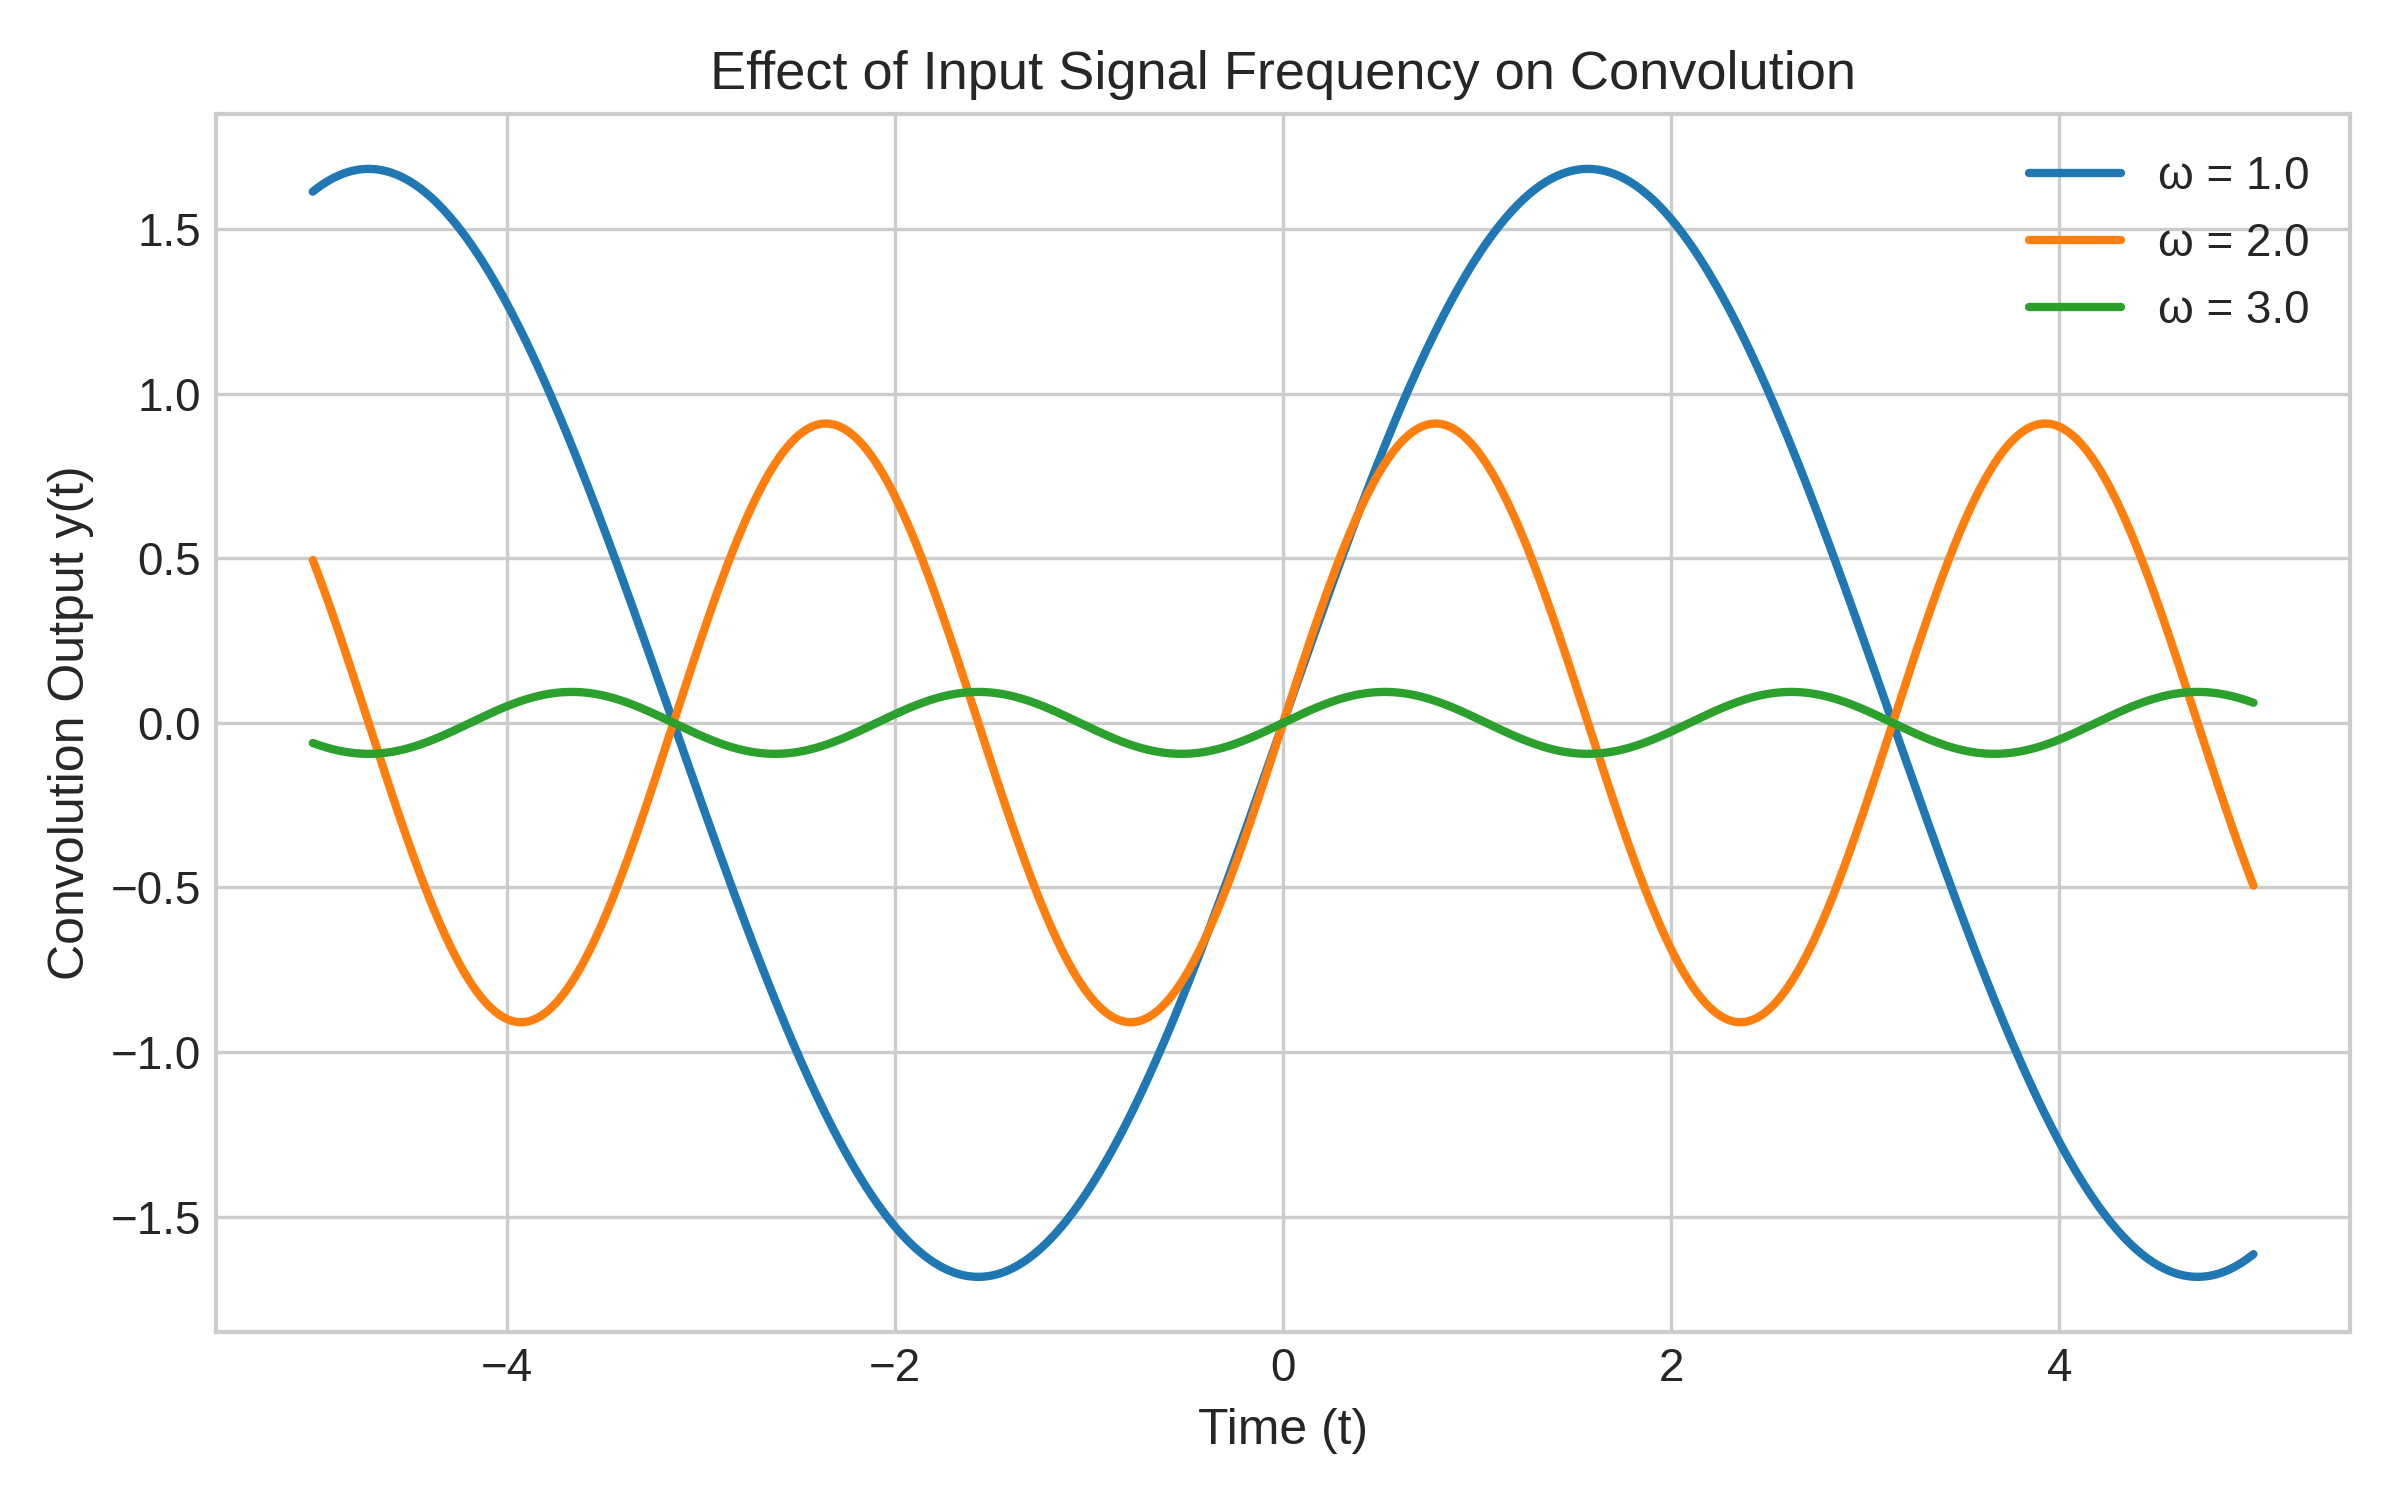
\includegraphics[width=0.8\textwidth]{codes/codes_sin_1_and_arcsin/figures/frequency_effect.png}
    \caption{Effect of varying input signal frequency on convolution output.}
    \label{fig:frequency}
\end{figure}

\subsubsection{Effect of Kernel Width}
The parameter $T$, which determines the kernel width, significantly impacts the convolution through the $\sin(\omega T)$ term in the amplitude factor. Figure \ref{fig:kernel} shows how different kernel widths affect the output.

\begin{figure}[H]
    \centering
    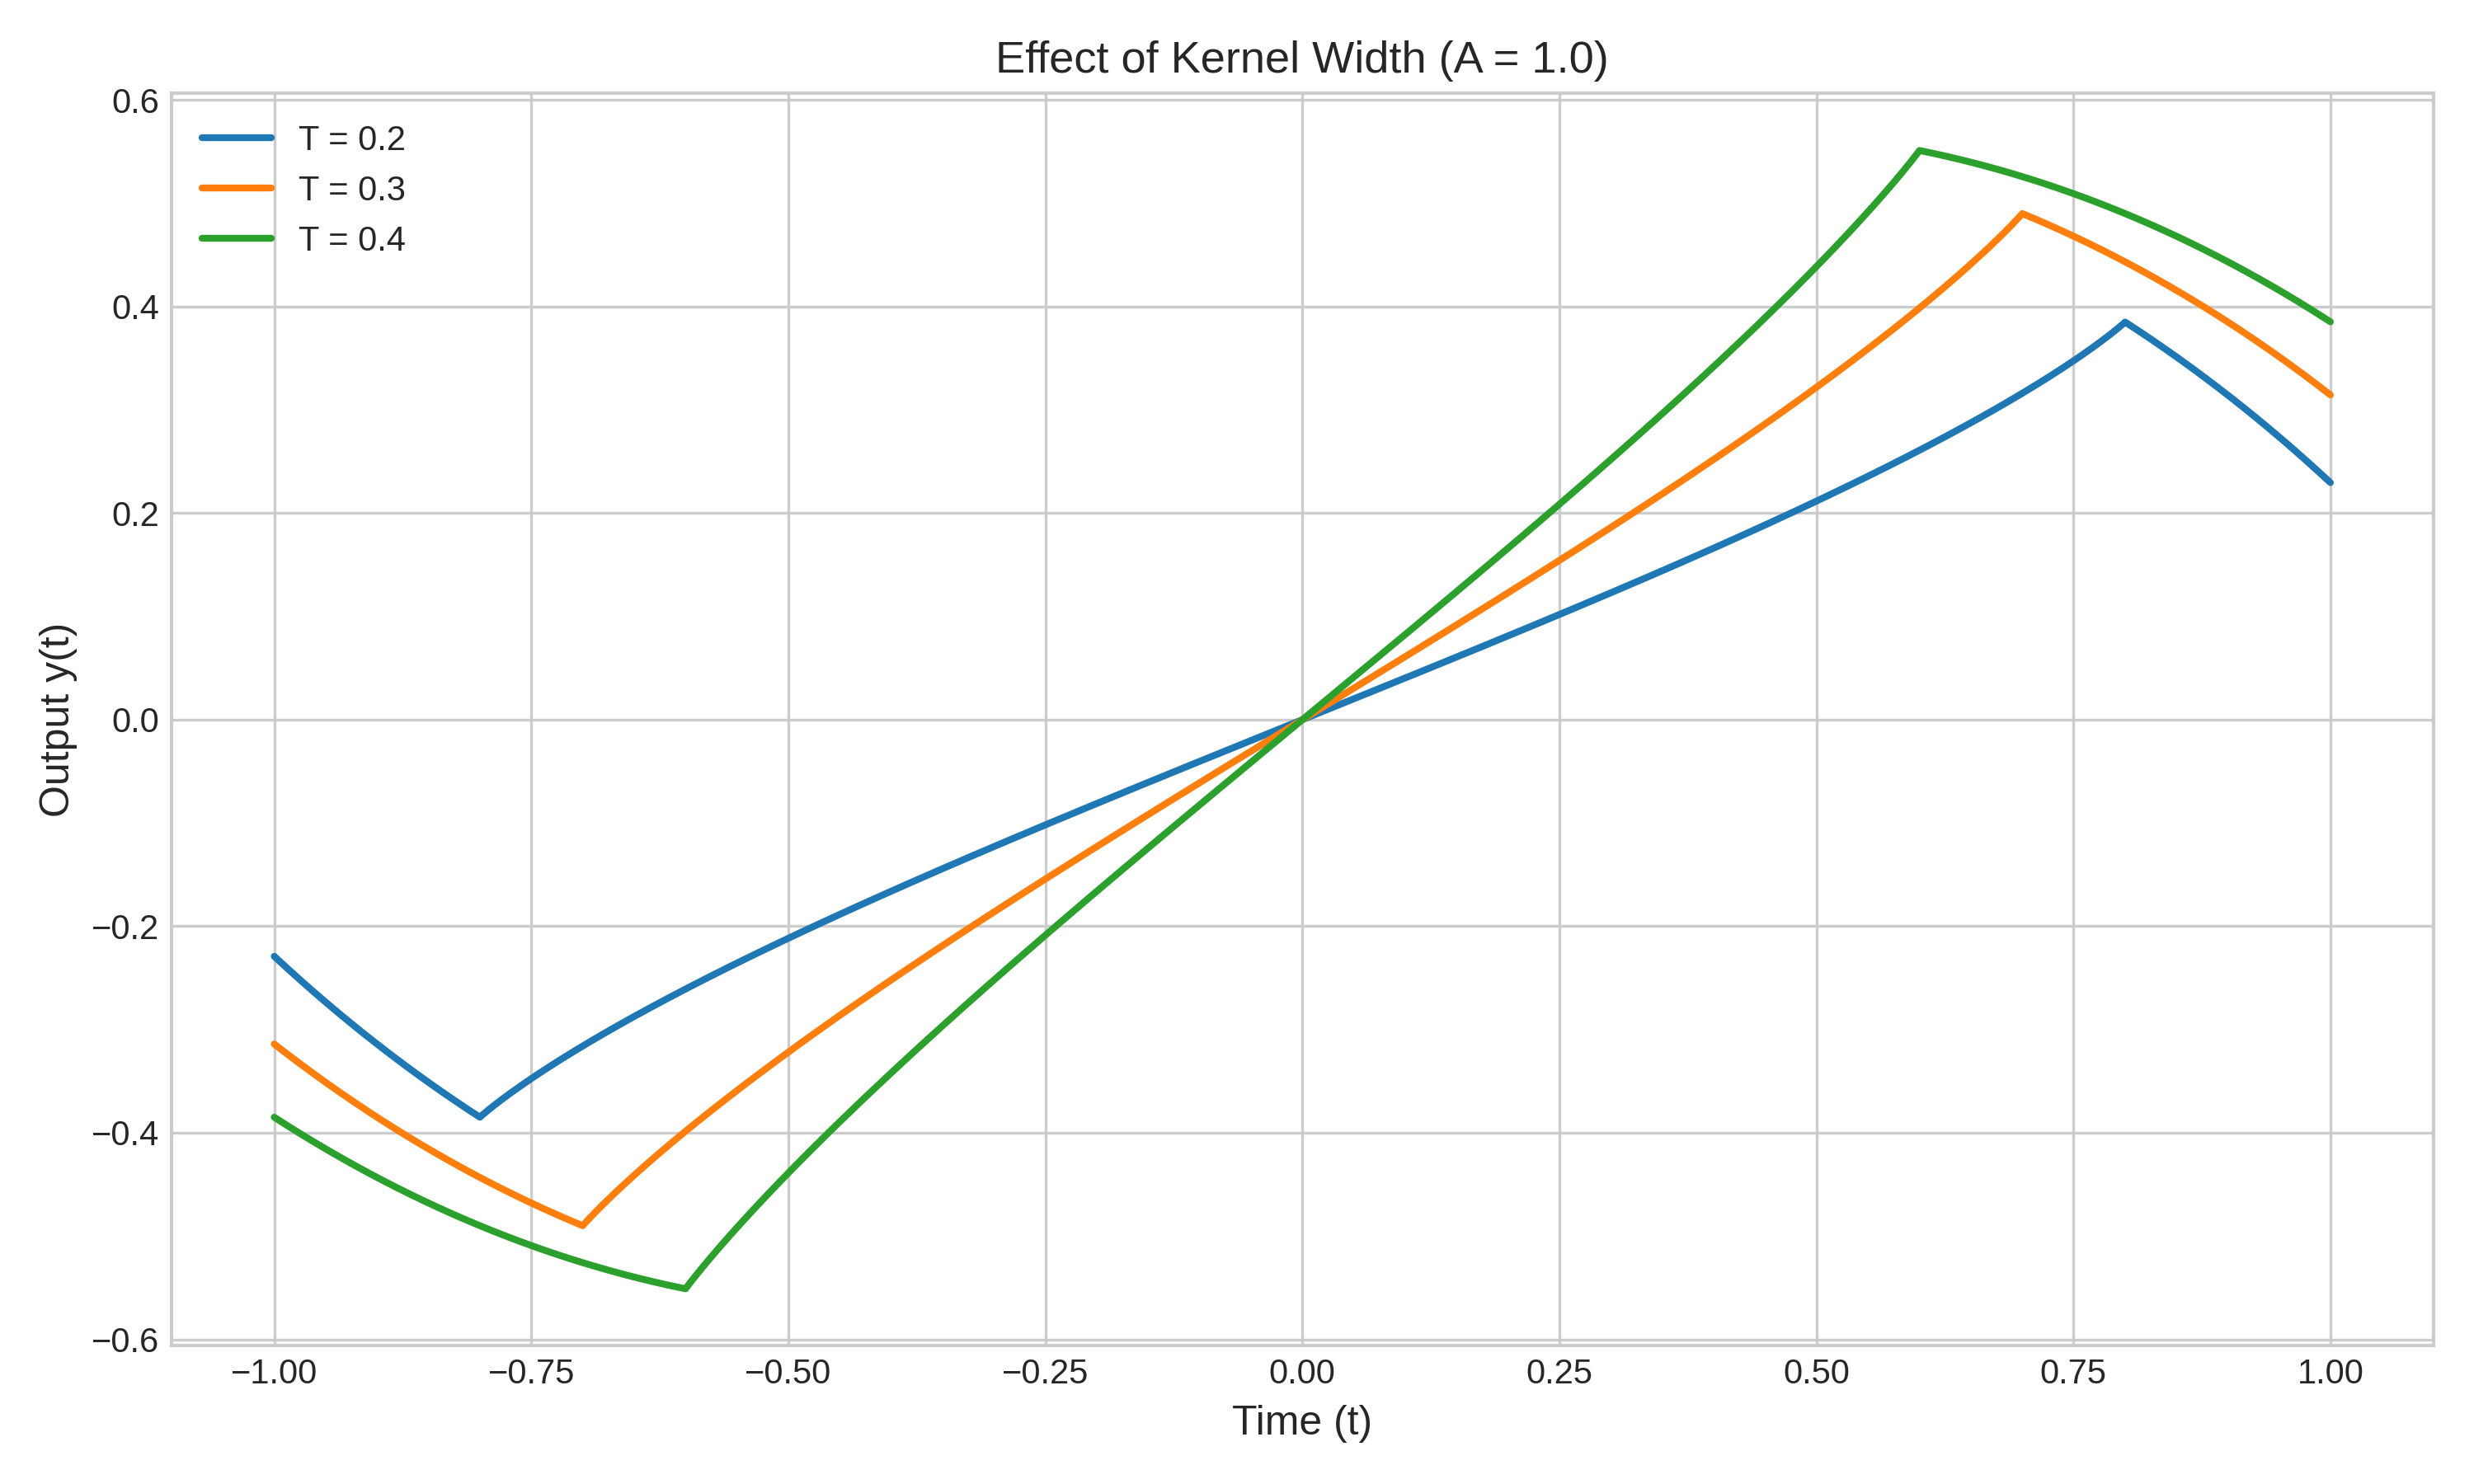
\includegraphics[width=0.8\textwidth]{codes/codes_sin_1_and_arcsin/figures/kernel_width_effect.png}
    \caption{Effect of varying kernel width on convolution output.}
    \label{fig:kernel}
\end{figure}


\subsection{Significance in Signal Processing}
These parameter dependencies reveal important practical implications:

\begin{itemize}
    \item The rectangular kernel acts as a frequency-selective filter, with the $\frac{2\sin(\omega T)}{\omega}$ term determining which frequencies pass through.
    
    \item The kernel width $T$ can be adjusted to target specific frequency ranges. Wider kernels (larger $T$) attenuate higher frequencies more strongly.
    
    \item The frequency nulls at $\omega T = n\pi$ demonstrate how certain combinations of input frequency and kernel width can completely eliminate signals.
    
    \item The system preserves the input signal's phase, which is important for maintaining signal timing relationships.
\end{itemize}

In practical applications, understanding these dependencies allows engineers to design appropriate filters for signal processing tasks or to predict how specific signal components will be affected by convolution operations.

\subsection{Conclusion}
The convolution of a sinusoidal signal with a rectangular kernel demonstrates key parameter dependencies that are fundamental to signal processing. The amplitude, frequency, and phase of the input signal, along with the kernel width, all influence the convolution output in specific ways. 

The most significant relationship is between the input frequency $\omega$ and kernel width $T$, which together determine whether signals are passed, attenuated, or completely nullified. This behavior forms the basis for filtering operations in many signal processing applications.

\section{Sinusoidal as $f(t)$ with Half-Box Kernel}

Compute the convolution of a given signal \( f(t) \) with a rectangular kernel \( h(t) \), analytically. The rectangular kernel is defined as:
\[
h(t) = 
\begin{cases}
1, & \text{for } -T \leq t \leq T, \\
0, & \text{otherwise}.
\end{cases}
\]
...

\subsection{Modify the kernel to only consider the part of the kernel for \( t > 0 \). How does this affect the convolution result?}

\subsubsection{Analytic}
In this analysis, we investigate the convolution of a sinusoidal input signal
\[
f(t) = A \sin(\omega t + \phi)
\]
with a rectangular kernel that is modified as below. The modified rectangular kernel is defined as:

\[
h(t) =
\begin{cases}
1, & \text{for } 0 < t < T, \\
0, & \text{otherwise}.
\end{cases}
\]

Our goal is to derive the convolution expression \( y(t) = (f \ast h)(t) \) analytically and analyze the system’s behavior.

The convolution of \( f(t) \) and \( h(t) \) is defined as:
\[
y(t) = (f \ast h)(t) = \int_{-\infty}^{\infty} f(\tau) h(t - \tau) \, d\tau
\]

Substituting our functions:
\[
y(t) = \int_{-\infty}^{\infty} A \sin(\omega \tau + \phi) \cdot h(t - \tau) \, d\tau
\]

Since the kernel \( h(t - \tau) \) is non-zero only when \( 0  < t - \tau <  T \), we can rewrite this condition as:
\[
t - T < \tau < t
\]

Therefore, the limits of integration become:
\[
y(t) = \int_{t - T}^{t} A \sin(\omega \tau + \phi) \, d\tau
\]

Evaluating this integral:
The integral of \( \sin(\omega \tau + \phi) \) is:
\[
\int \sin(\omega \tau + \phi) \, d\tau = -\frac{1}{\omega} \cos(\omega \tau + \phi)
\]

Evaluating the integral from \( t - T \) to \( t \):
\[
y(t) = A \left[ -\frac{1}{\omega} \cos(\omega \tau + \phi) \right]_{t - T}^{t}
\]

This simplifies to:
\[
y(t) = A \left( -\frac{1}{\omega} \cos(\omega t + \phi) + \frac{1}{\omega} \cos(\omega (t - T) + \phi) \right)
\]
Using the identity for the difference of cosines:
\[
\cos A - \cos B = -2 \sin\left( \frac{A + B}{2} \right) \sin\left( \frac{A - B}{2} \right)
\]
\[
y(t) = \frac{A}{\omega} \left( -2 \sin \left( \frac{(\omega (t - T) + \phi) + (\omega t + \phi)}{2} \right) \sin \left( \frac{(\omega (t - T) + \phi) - (\omega t + \phi)}{2} \right) \right)
\]
\[
y(t) = \frac{A}{\omega} \left( -2 \sin \left( \omega t + \phi - \frac{\omega T}{2} \right) \sin \left( \frac{\omega T}{2} \right) \right)
\]
\[
\boxed{y(t) = \frac{2A \sin\left( \frac{\omega T}{2} \right)}{\omega} \sin \left( \omega( t  - \frac{T}{2}) + \phi \right)}
\]
The convolution for the modified kernel does not change the behavior of the signal, i.e., the output still remains sinusoidal.The significant differences are as follows :
\begin{itemize}
\item A $ \frac{T}{2} $ time shift towards right .

\item The scaling of amplitude is changed from $\frac{2\sin(\omega T)}{\omega}$ to $\frac{2\sin(\frac{\omega T}{2})}{\omega}$ .
\end{itemize}

\begin{figure}
    \centering
    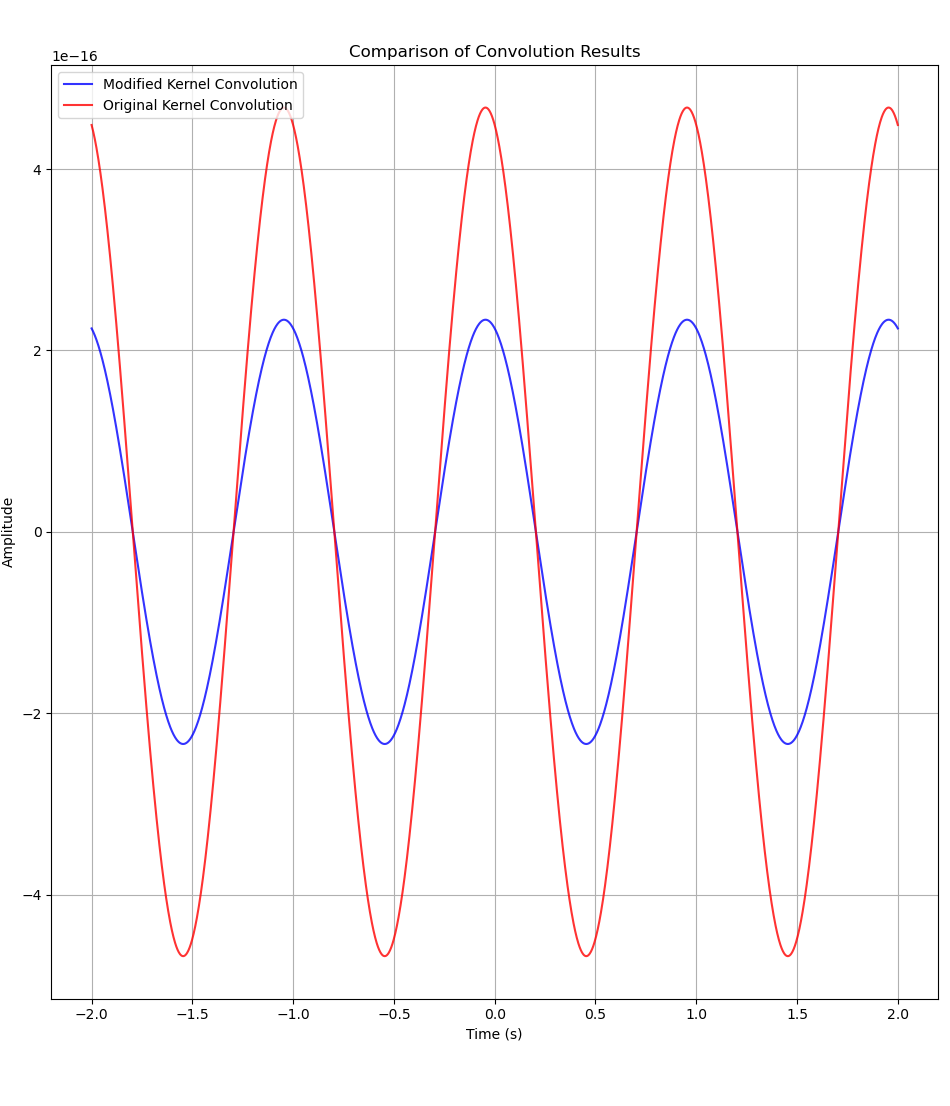
\includegraphics[width=0.5\linewidth]{codes/codes_sin_2/figs/compare.png}
    \caption{Plot of the convolutions}
    \label{fig:enter-label}
\end{figure}

\newpage

\subsection{Extended Graphical and Analytical Analysis}

\subsubsection{Effect of Amplitude \( A \)}

The first figure below demonstrates the impact of changing amplitude values on the convolution result. As seen, increasing the amplitude scales the overall magnitude of the output signal, keeping the shape unchanged.
\begin{figure}[h]
    \centering
    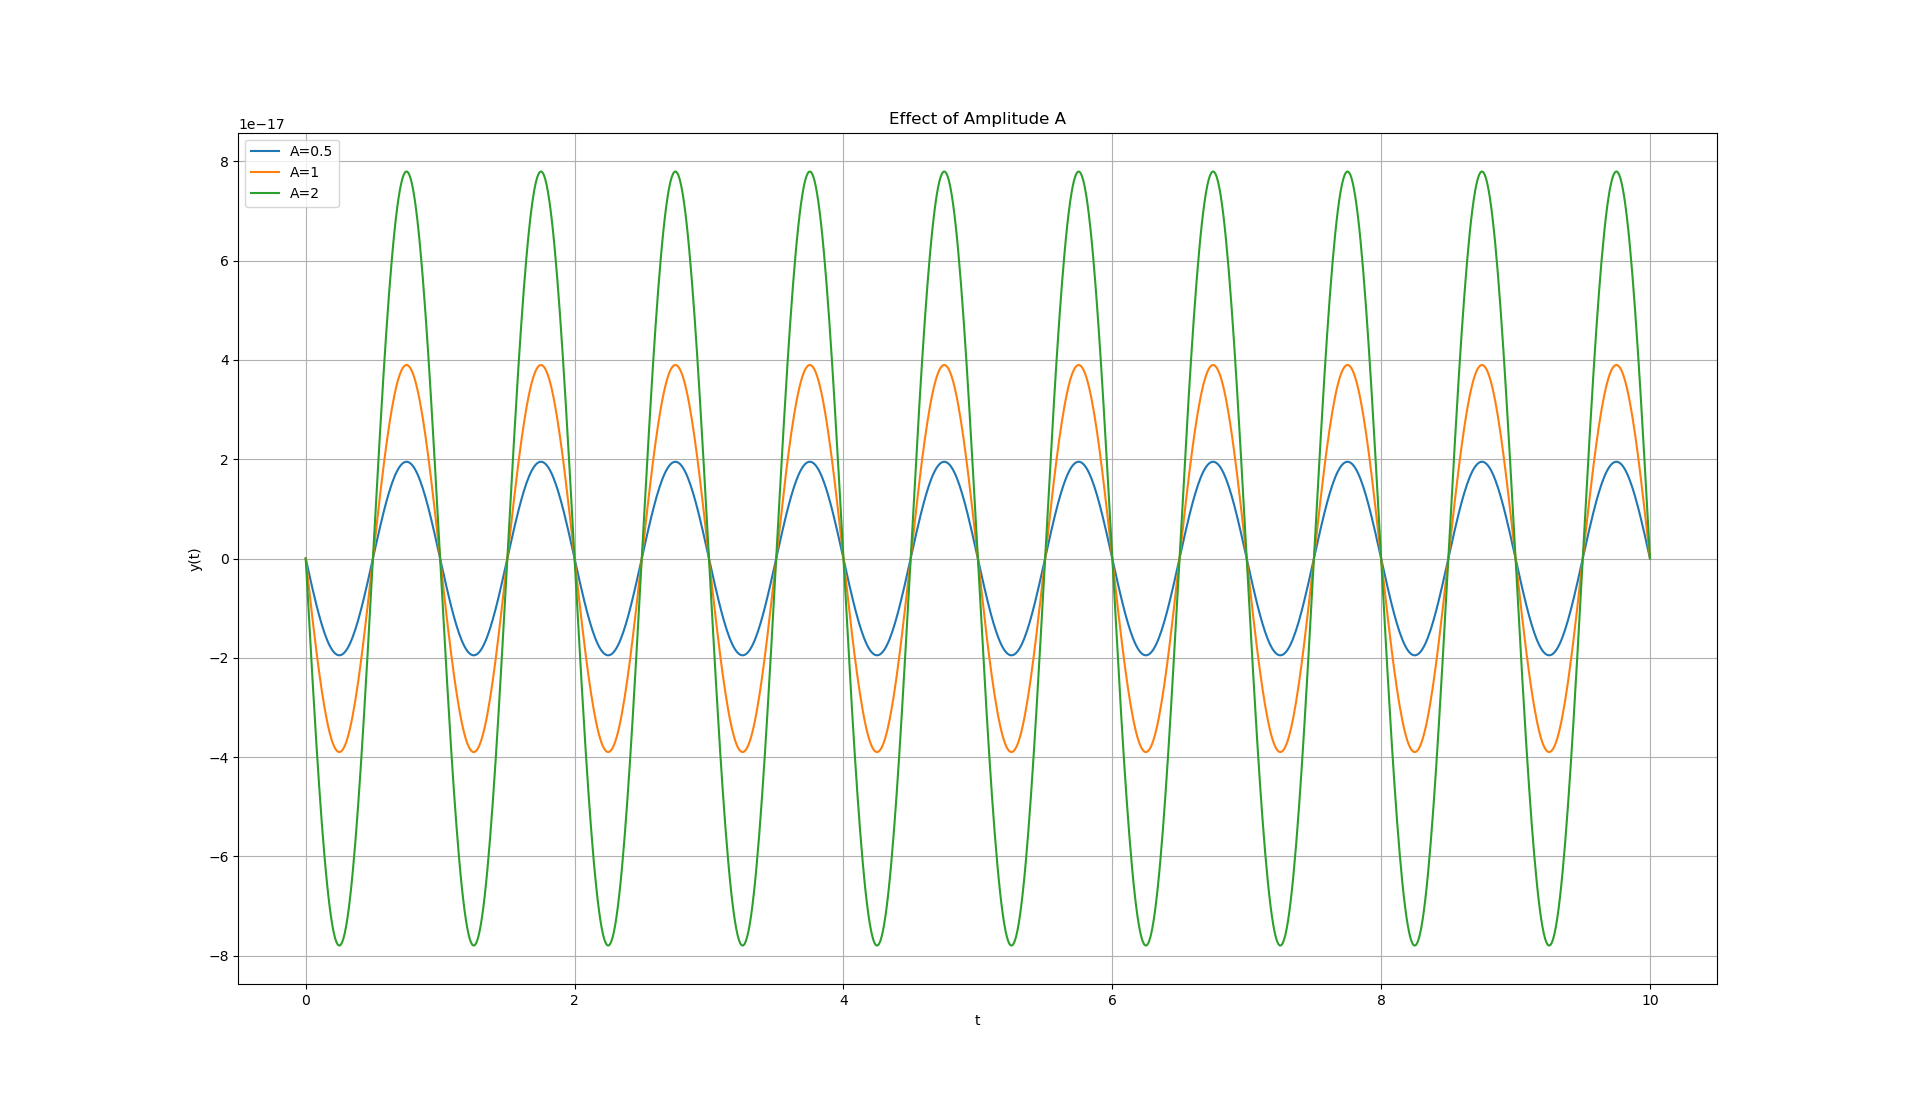
\includegraphics[width=0.8\textwidth]{codes/codes_sin_2/figs/amp.png}
    \caption{Effect of varying amplitude \( A \) on the convolution output.}
\end{figure}



\subsubsection{Effect of Angular Frequency \( \omega \)}

Changing \( \omega \) changes how rapidly the sinusoidal input oscillates. This figure shows how higher frequencies start diminishing in magnitude due to the sinc-type attenuation from the convolution.
\begin{figure}[h]
    \centering
    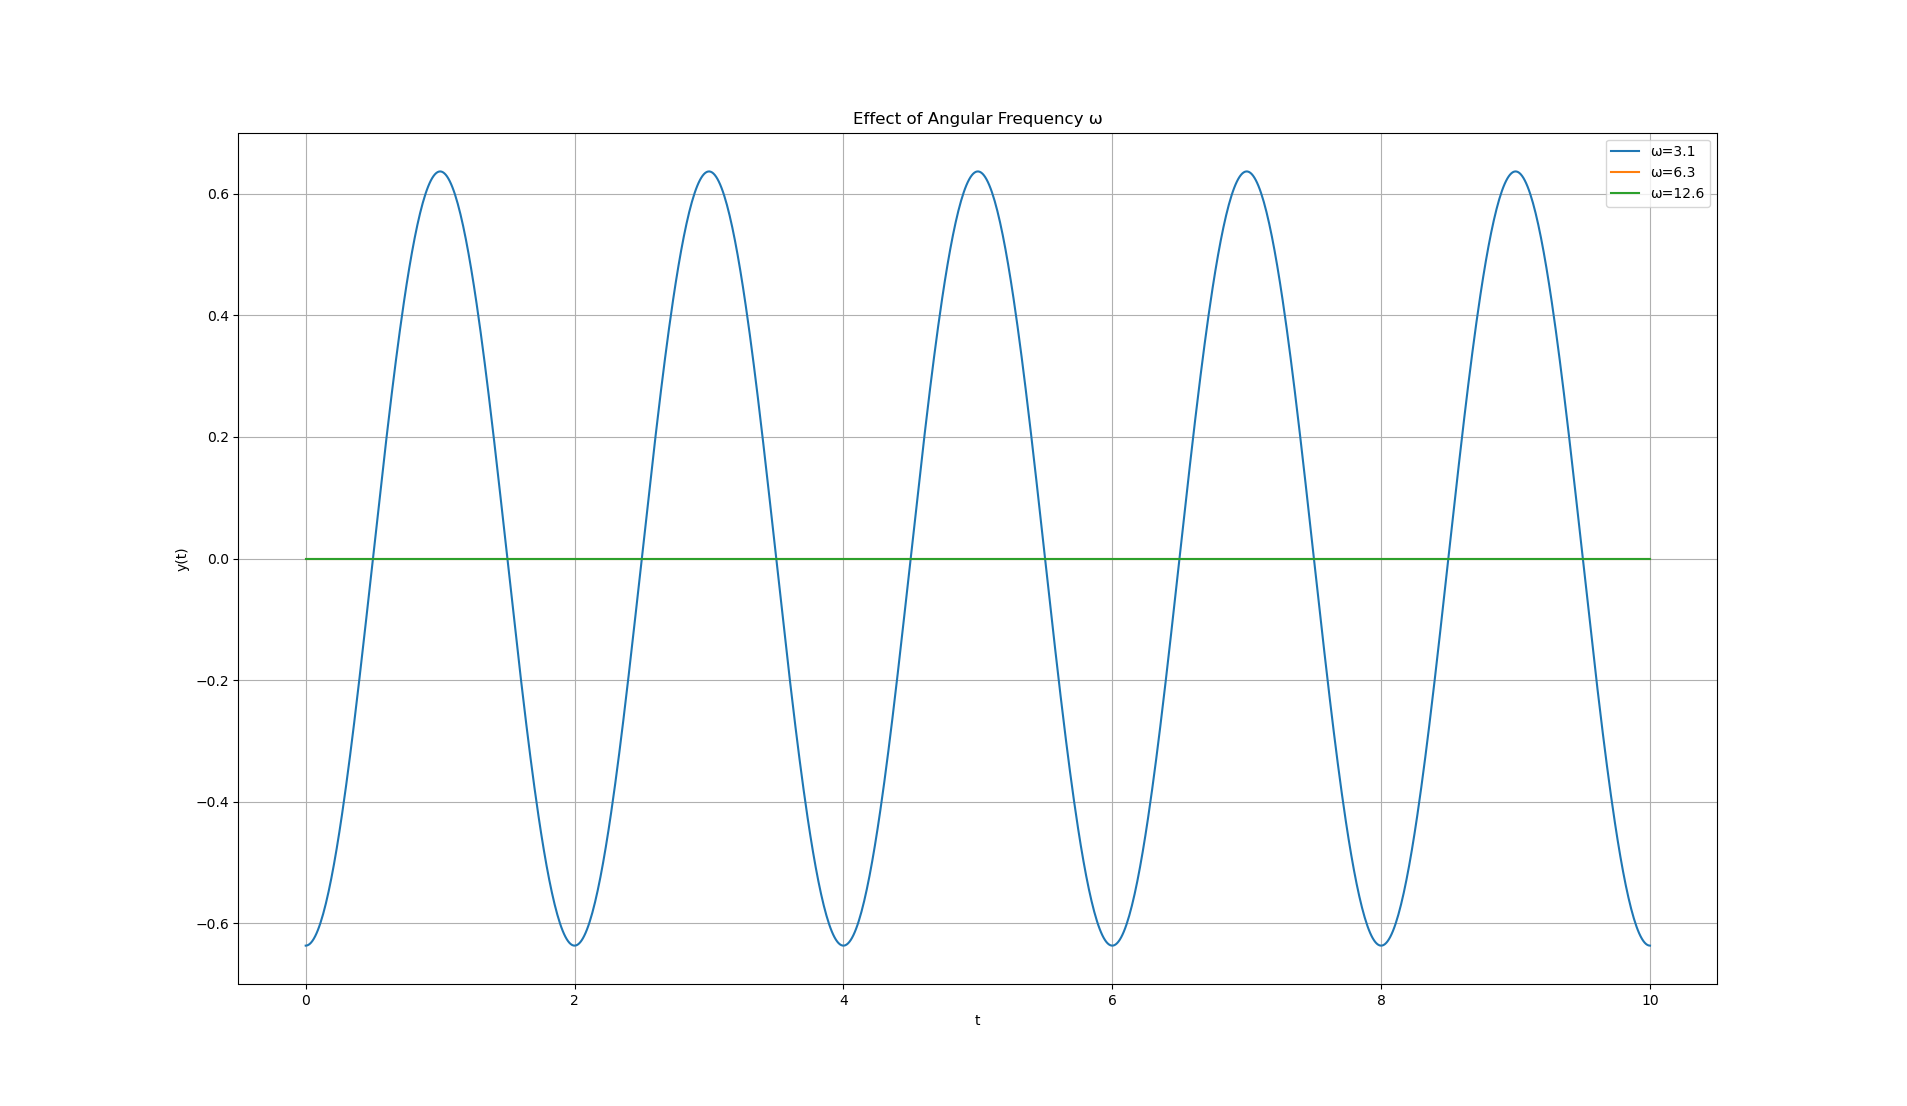
\includegraphics[width=0.8\textwidth]{codes/codes_sin_2/figs/omega.png}
    \caption{Effect of angular frequency \( \omega \) on convolution. Higher frequencies are attenuated.}
\end{figure}

\subsubsection{Effect of Pulse Width \( T \)}

This graph demonstrates how varying \( T \), the width of the rectangular kernel, influences the output. Smaller \( T \) leads to lesser averaging, preserving high-frequency content. Larger \( T \) results in more smoothing.
\begin{figure}[h]
    \centering
    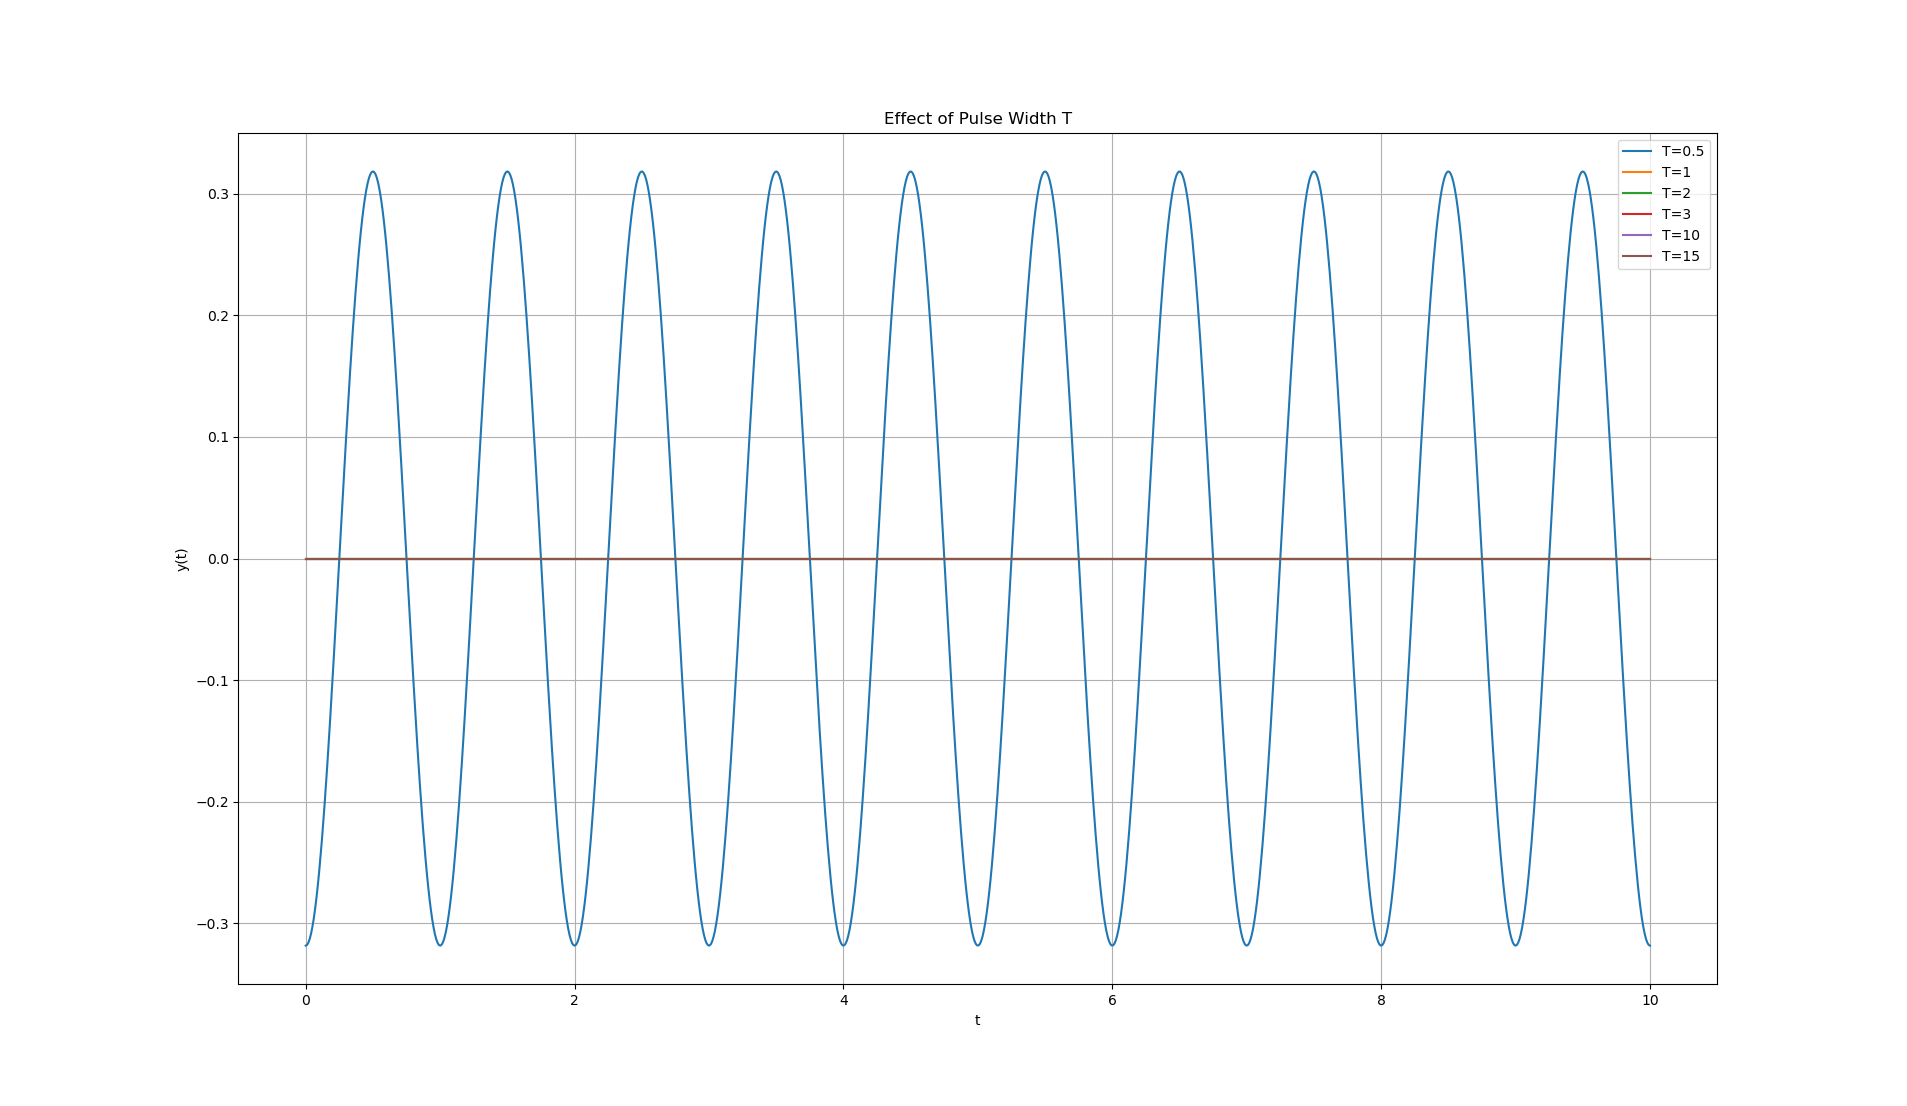
\includegraphics[width=0.8\textwidth]{codes/codes_sin_2/figs/T.png}
    \caption{Convolution output for different pulse widths \( T \).}
\end{figure}

\subsubsection{Amplitude Ratio vs Angular Frequency}

This plot captures the normalized amplitude ratio \( \frac{A_{out}}{A} = \frac{2\sin(\omega \frac{T}{2})}{\omega} \) as a function of \( \omega \) for various values of \( T \). It reflects the sinc-function behavior, emphasizing low-pass characteristics of convolution with rectangular kernels.
\begin{figure}[h]
    \centering
    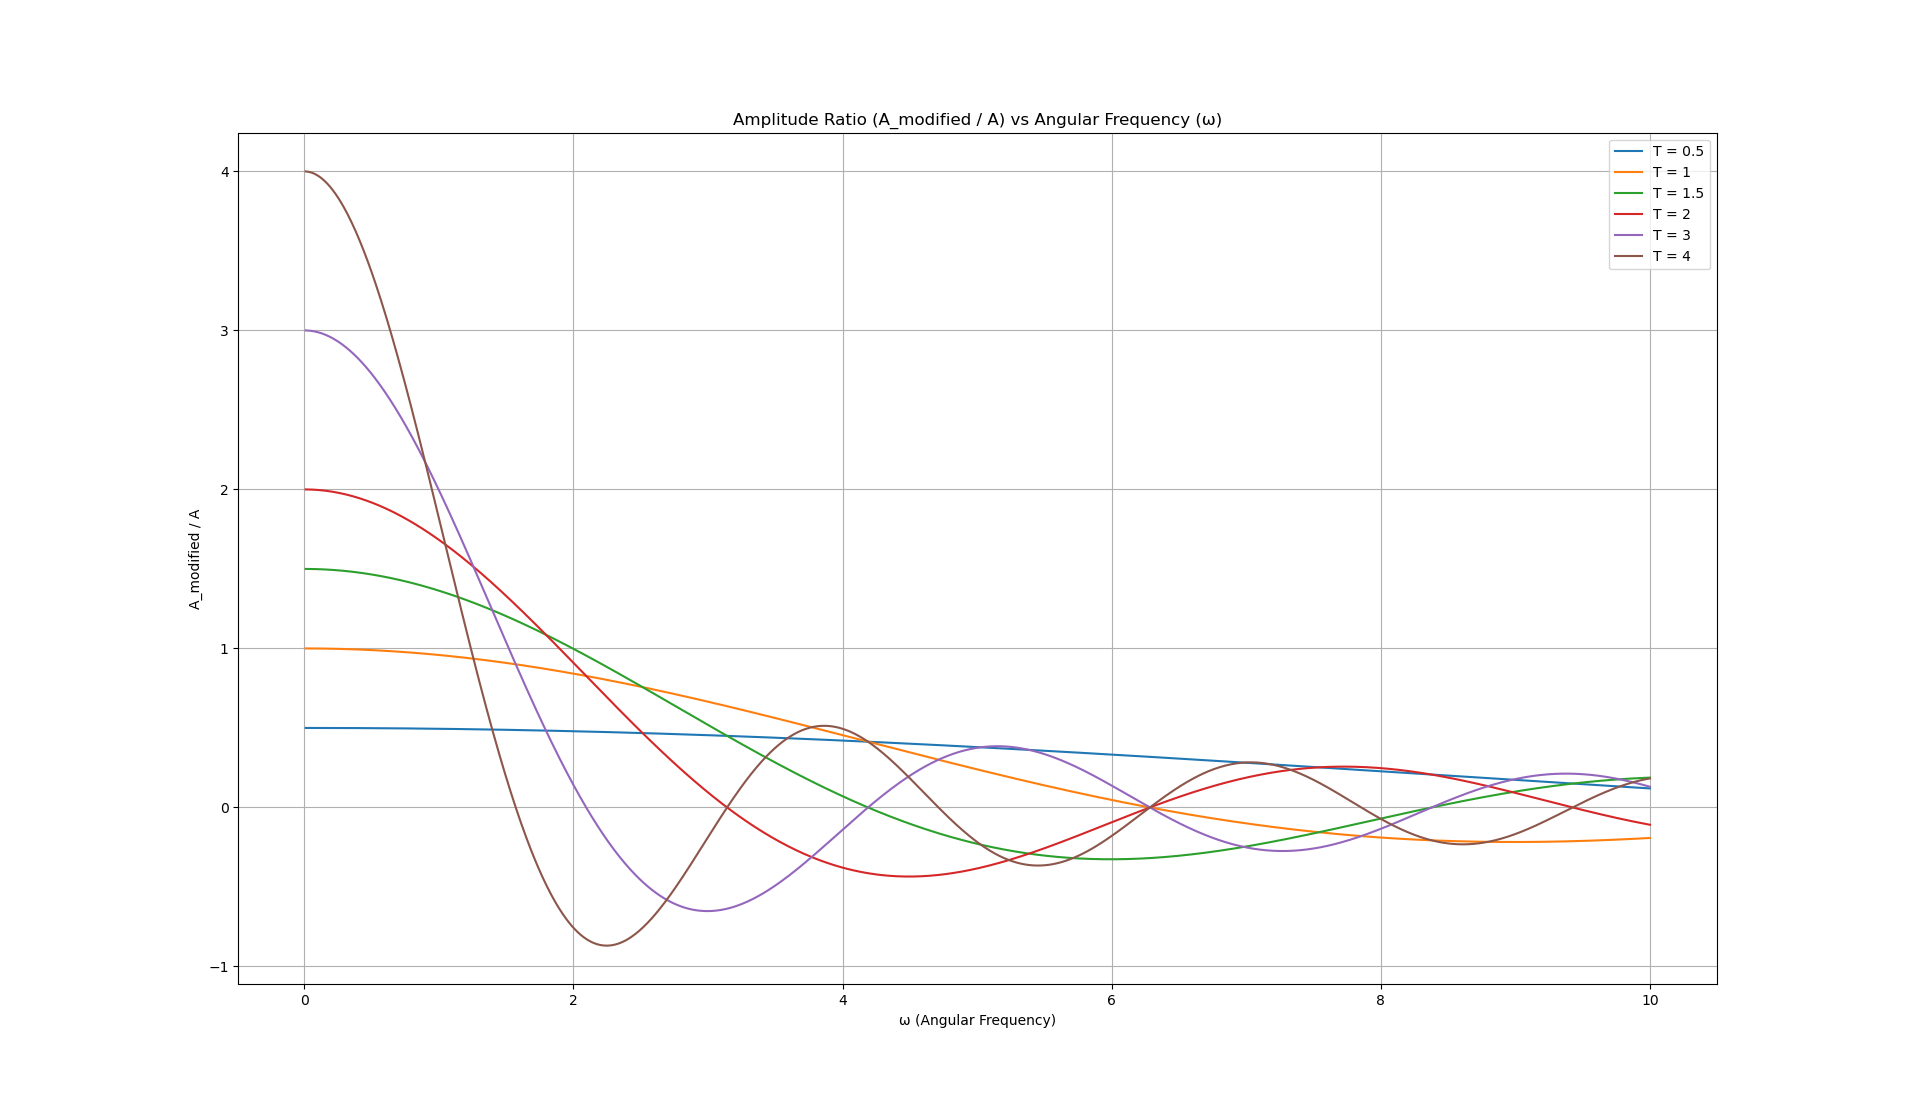
\includegraphics[width=0.8\textwidth]{codes/codes_sin_2/figs/scaling.png}
    \caption{Amplitude ratio \( \frac{A_{\text{modified}}}{A} \) versus angular frequency \( \omega \) for different values of \( T \).}
\end{figure}

\subsubsection{Effect of Phase \( \phi \)}

Altering the phase \( \phi \) of the sinusoidal signal results in horizontal shifts in the waveform. The output retains its shape but is delayed or advanced in time.
\begin{figure}[h]
    \centering
    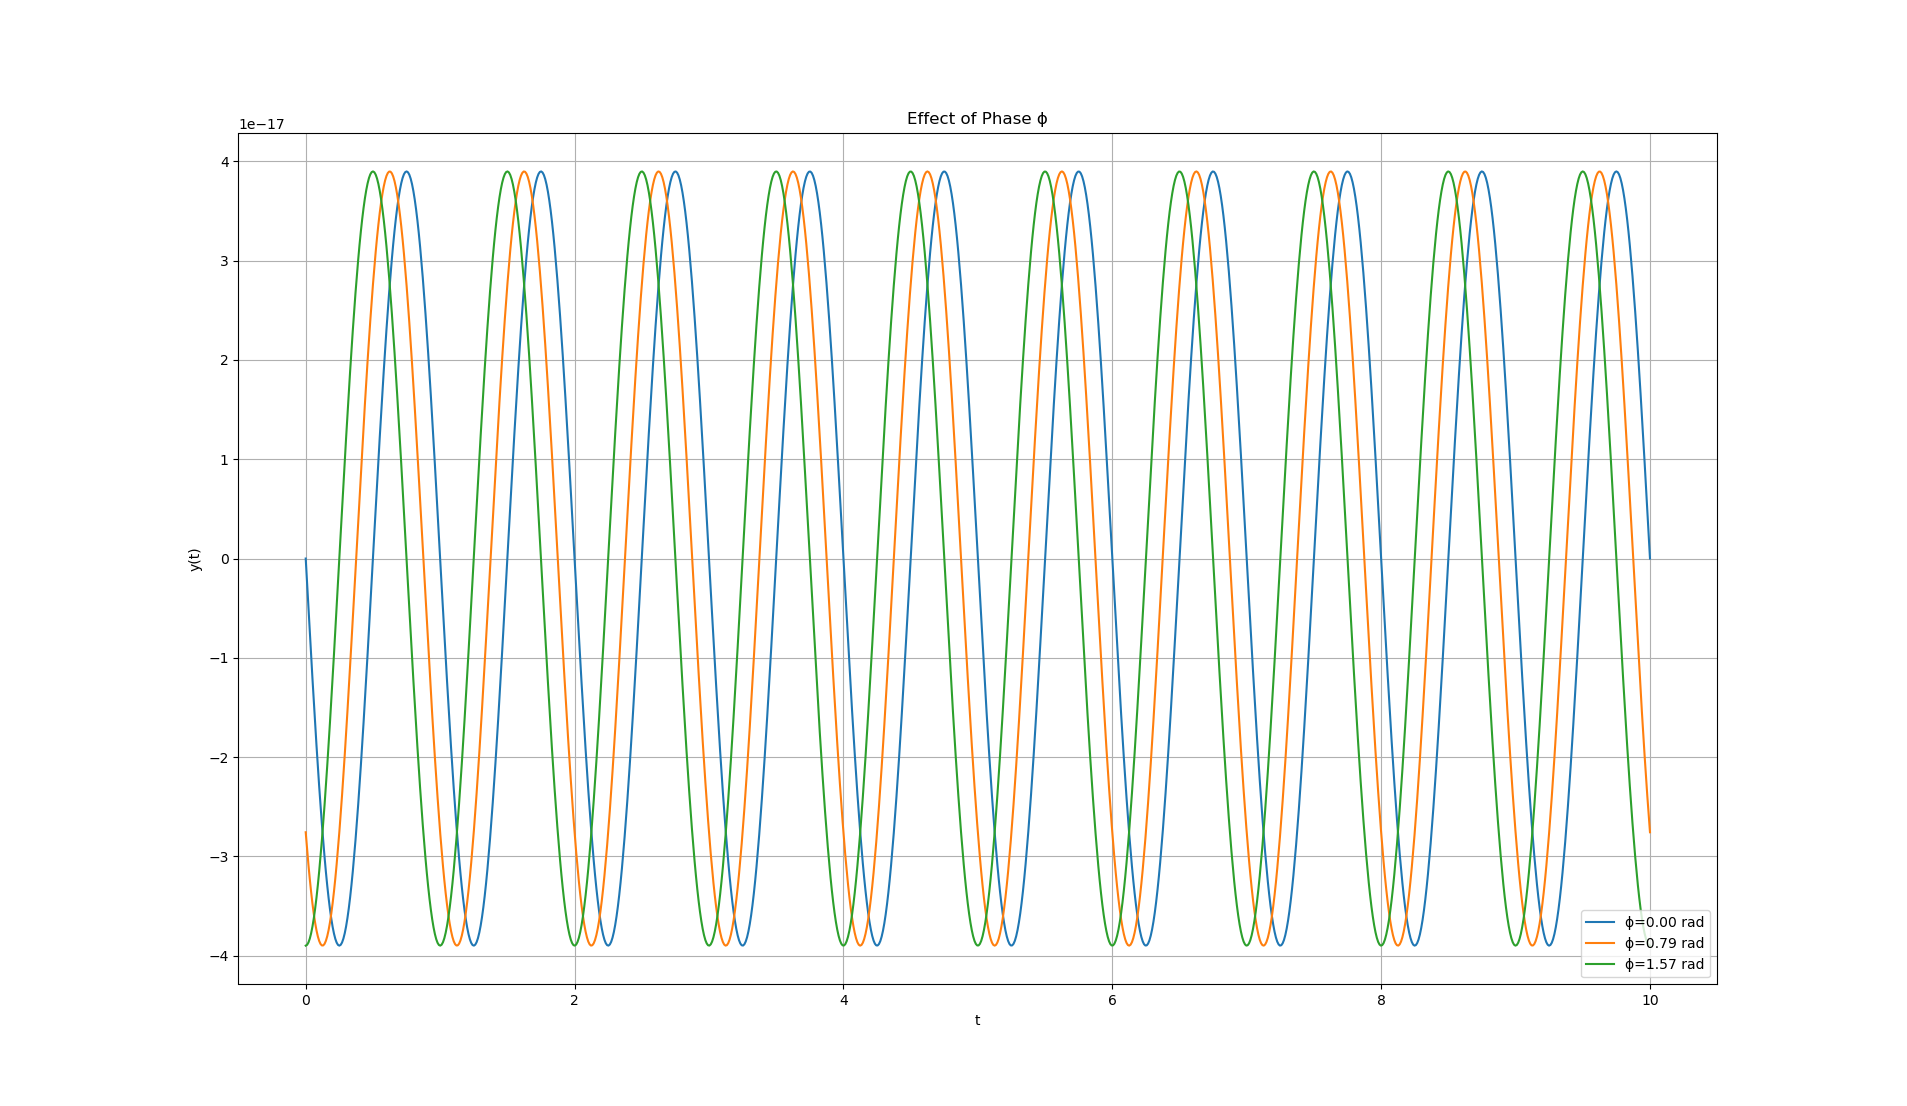
\includegraphics[width=0.8\textwidth]{codes/codes_sin_2/figs/phi.png}
    \caption{Phase shift \( \phi \) changes the horizontal alignment of the output signal.}
\end{figure}

\subsubsection{Special Observations}
\begin{itemize}
    \item If \( \omega T = n\pi \), the output vanishes, indicating frequency nulls.
    \item For large \( T \), the kernel acts as a low-pass filter.
    \item When \( T \rightarrow 0 \), the kernel approximates an impulse, and the convolution result tends to zero everywhere.
\end{itemize}

\subsection{Convolution with Varying Parameters}

The figure below shows the convolution output for multiple combinations of parameters including amplitude \( A \), frequency \( \omega \), kernel width \( T \), and phase \( \phi \). It highlights how these parameters influence the shape, scaling, and shift of the output signal.

Each sub-plot or curve within the figure corresponds to a unique configuration. You can observe:
\begin{itemize}
    \item Changes in amplitude due to scaling by \( \frac{2\sin(\omega T)}{\omega} \)
    \item Phase shifts resulting from both the signal phase \( \phi \) and kernel delay \( \tau_0 \)
    \item Smoothing effects due to increasing kernel width \( T \)
    \item Attenuation of high-frequency components, emphasizing the low-pass filter nature of box kernels
\end{itemize}

\begin{figure}[h]
    \centering
    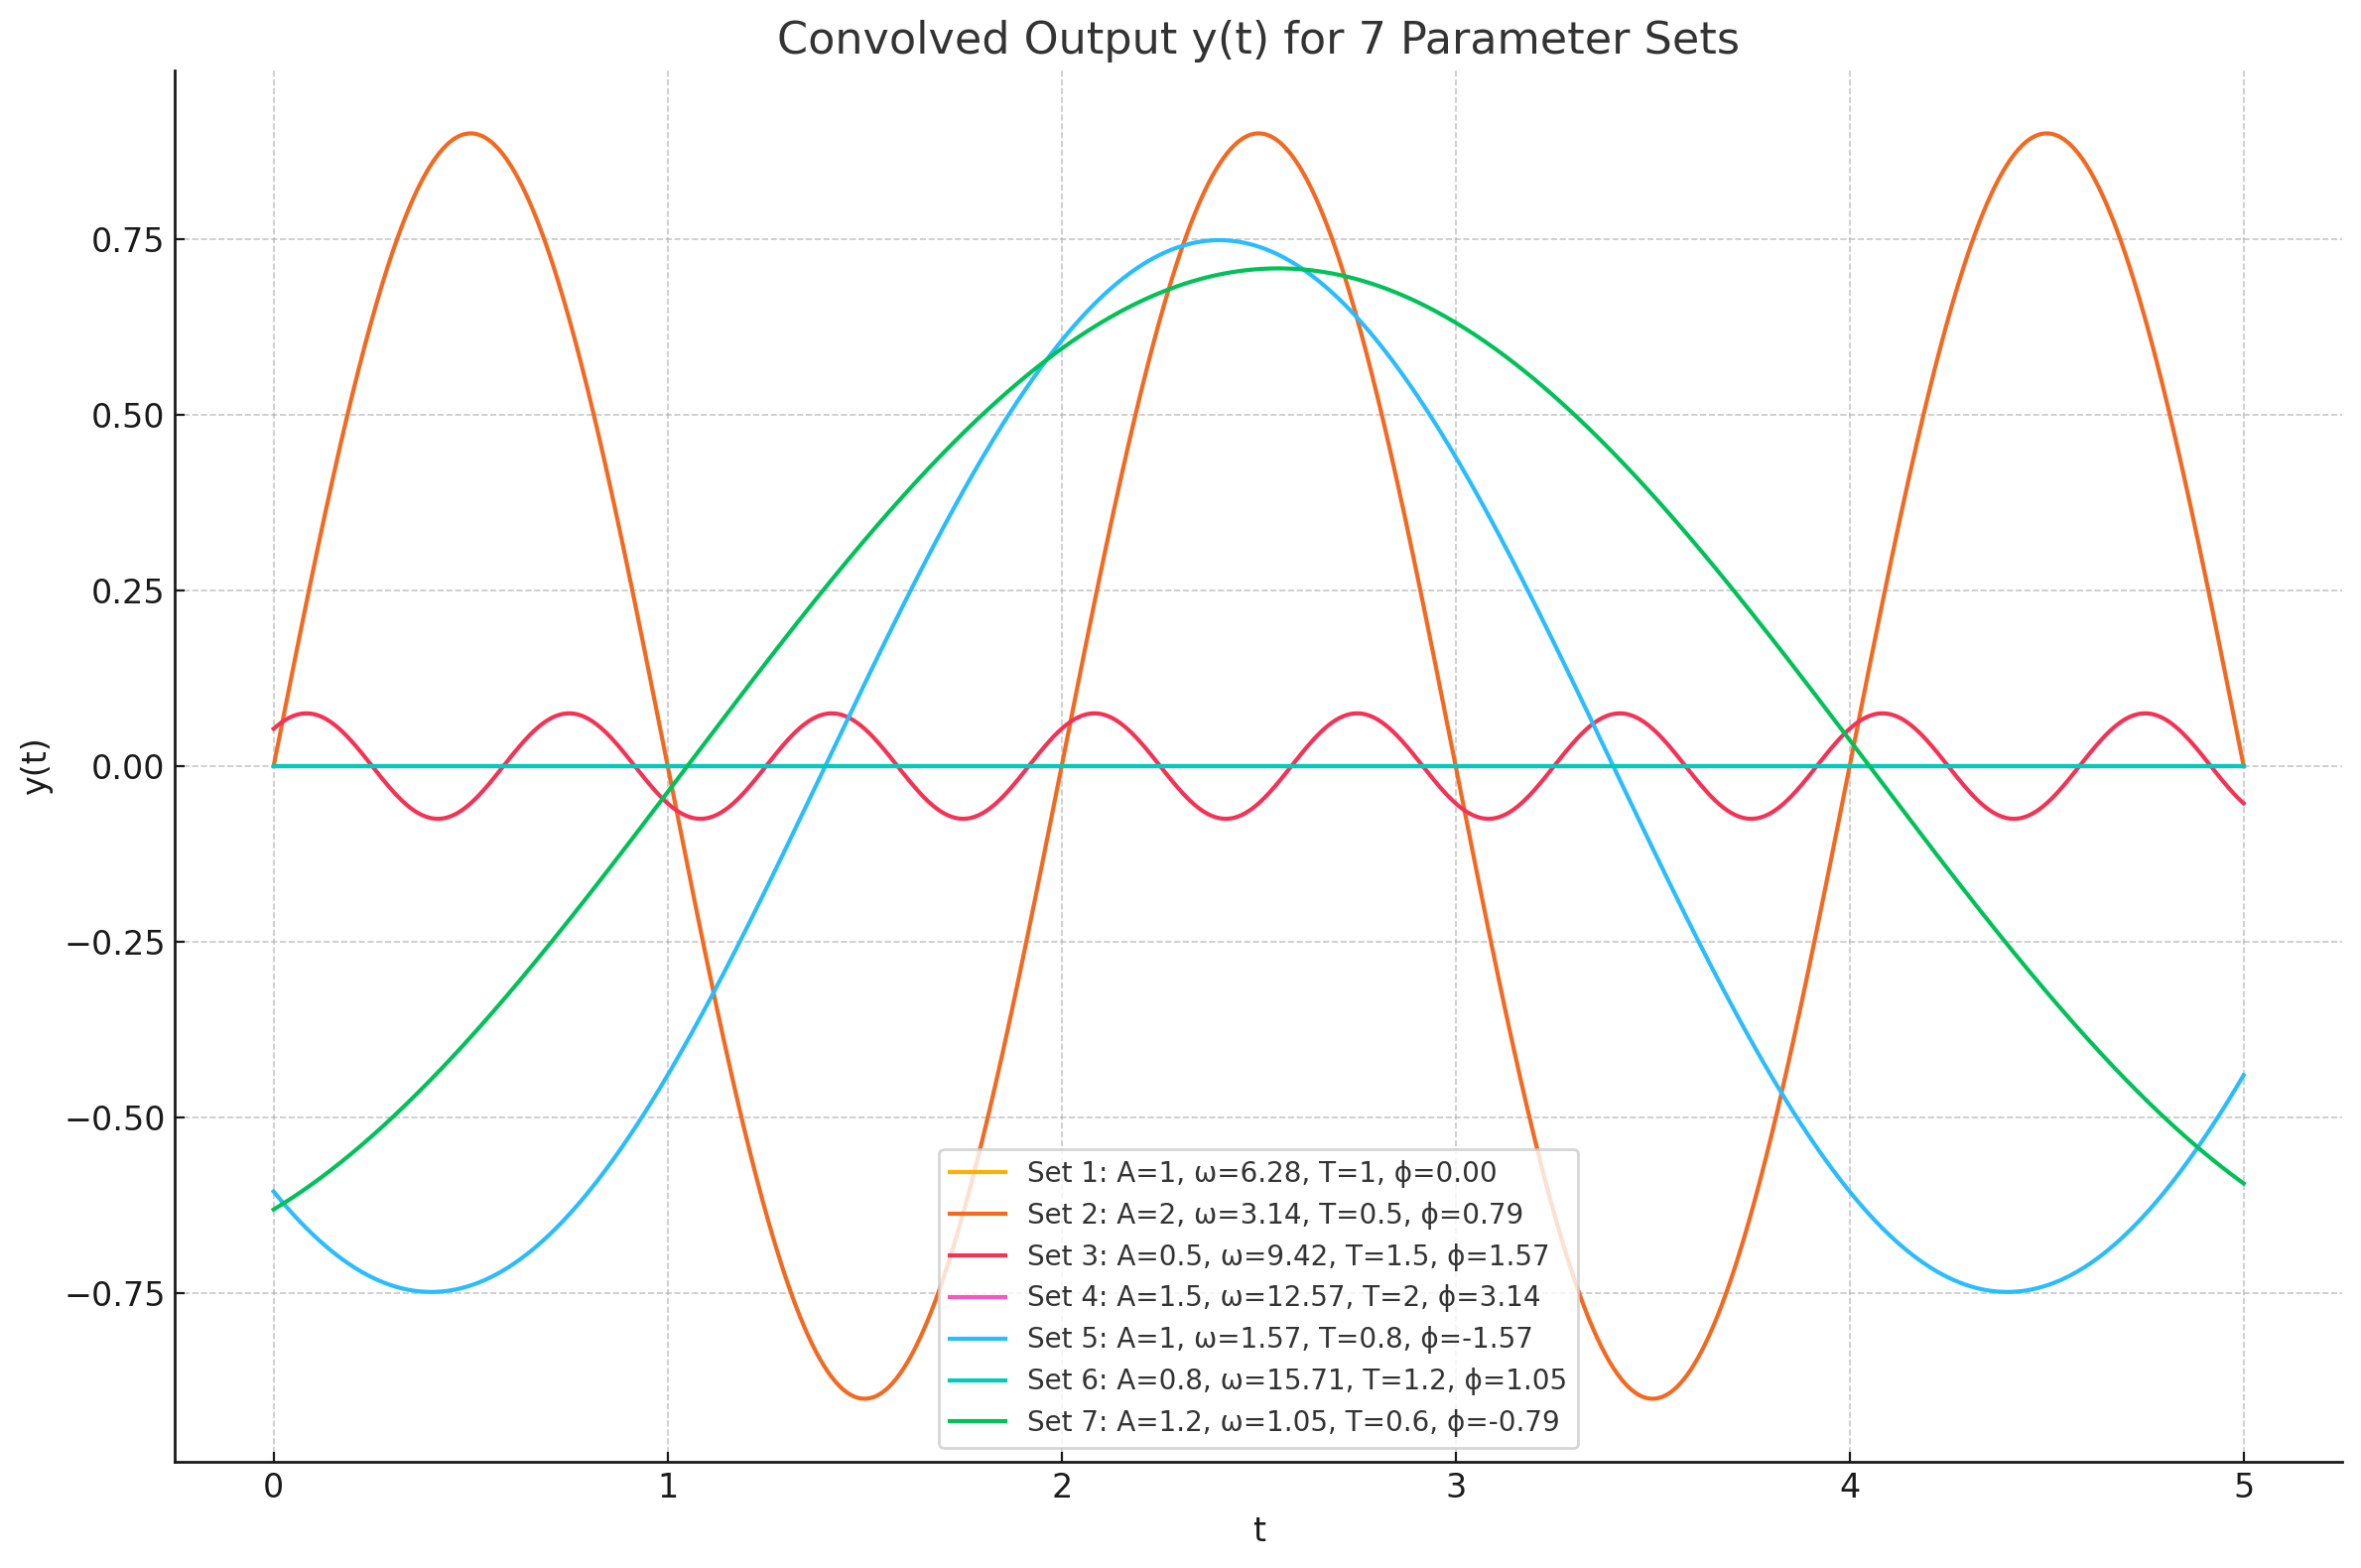
\includegraphics[width=0.7\textwidth]{codes/codes_sin_2/figs/all_varies.png}
    \caption{Convolution output for different parameter sets \( (A, \omega, T, \phi) \).}
\end{figure}


\subsection{Conclusion}

This detailed analysis of convolution using a rectangular kernel shows how parameters such as amplitude, frequency, kernel width, and phase influence the output signal. The kernel acts as a smoothing and low-pass filter, selectively attenuating high-frequency components. Additionally, time-shifting the kernel leads to equivalent shifts in the output, demonstrating important system properties like linearity and time invariance.

\end{document}

\section{Sinusoidal $f(t)$ with Shifted Time Box Kernel}
In this analysis, we investigate the convolution of a sinusoidal input signal $f(t) = A\sin(\omega t + \phi)$ with a rectangular kernel that is shifted by $\tau_0$. The shifted rectangular kernel is defined as:

$$
h(t)= \begin{cases}
1, & \text{for } \tau_0-T < t < \tau_0+T \\
0, & \text{otherwise}
\end{cases}
$$

Our goal is to derive the convolution expression $y(t)=(f * h)(t)$ analytically and analyze the system's behavior.

\subsection{Analytical Derivation}

The convolution of $f(t)$ and $h(t)$ is defined as:

$$
y(t) = (f * h)(t) = \int_{-\infty}^{\infty} f(\tau)h(t-\tau)d\tau
$$

Substituting our functions:

$$
y(t) = \int_{-\infty}^{\infty} A\sin(\omega \tau + \phi) \cdot h(t-\tau)d\tau
$$

Since the kernel $h(t-\tau)$ is non-zero only when $\tau_0-T < t-\tau < \tau_0+T$, we can rewrite this as:

$$
t-\tau_0-T < \tau < t-\tau_0+T
$$

Therefore, the limits of integration become:

$$
y(t) = \int_{t-\tau_0-T}^{t-\tau_0+T} A\sin(\omega \tau + \phi)d\tau
$$

Evaluating this integral:

\begin{align*}
y(t) &= A\int_{t-\tau_0-T}^{t-\tau_0+T} \sin(\omega \tau + \phi)d\tau \\
&= -\frac{A}{\omega}[\cos(\omega \tau + \phi)]_{t-\tau_0-T}^{t-\tau_0+T} \\
&= -\frac{A}{\omega}[\cos(\omega(t-\tau_0+T) + \phi) - \cos(\omega(t-\tau_0-T) + \phi)]
\end{align*}

Using the trigonometric identity $\cos(\alpha) - \cos(\beta) = -2\sin\left(\frac{\alpha+\beta}{2}\right)\sin\left(\frac{\alpha-\beta}{2}\right)$:

\begin{multline*}
    y(t) = -\frac{A}{\omega}\left[-2\sin\left(\frac{\omega(t-\tau_0+T) + \phi + \omega(t-\tau_0-T) + \phi}{2}\right)\right] \\ \left[\sin\left(\frac{\omega(t-\tau_0+T) + \phi - (\omega(t-\tau_0-T) + \phi)}{2}\right)\right]
\end{multline*}
\begin{align*}
y(t) &= -\frac{A}{\omega}\left[-2\sin(\omega(t-\tau_0) + \phi)\sin(\omega T)\right] \\
    \implies y(t) &= \frac{2A\sin(\omega T)}{\omega}\sin(\omega(t-\tau_0) + \phi)
\end{align*}

We can see that this result is similar to the case where shift does not happen. The main difference which is seen that the convolution output is shifted by an exact amounnt $\tau_0$.

\subsection{Analysis of the Result}

The convolution result can be expressed as:

$$
y(t) = \frac{2A\sin(\omega T)}{\omega}\sin(\omega(t-\tau_0) + \phi)
$$

This shows that:

\begin{enumerate}
\item The output is still a sinusoidal function with the same frequency $\omega$ as the input.

\item The amplitude is scaled by a factor of $\frac{2\sin(\omega T)}{\omega}$, which depends on both the frequency of the input signal and the half-width $T$ of the rectangular kernel.

\item The phase of the output signal is shifted by $\tau_0$, which corresponds to the shift in the rectangular kernel.

\end{enumerate}

\begin{figure}[!ht]
    \begin{center}
        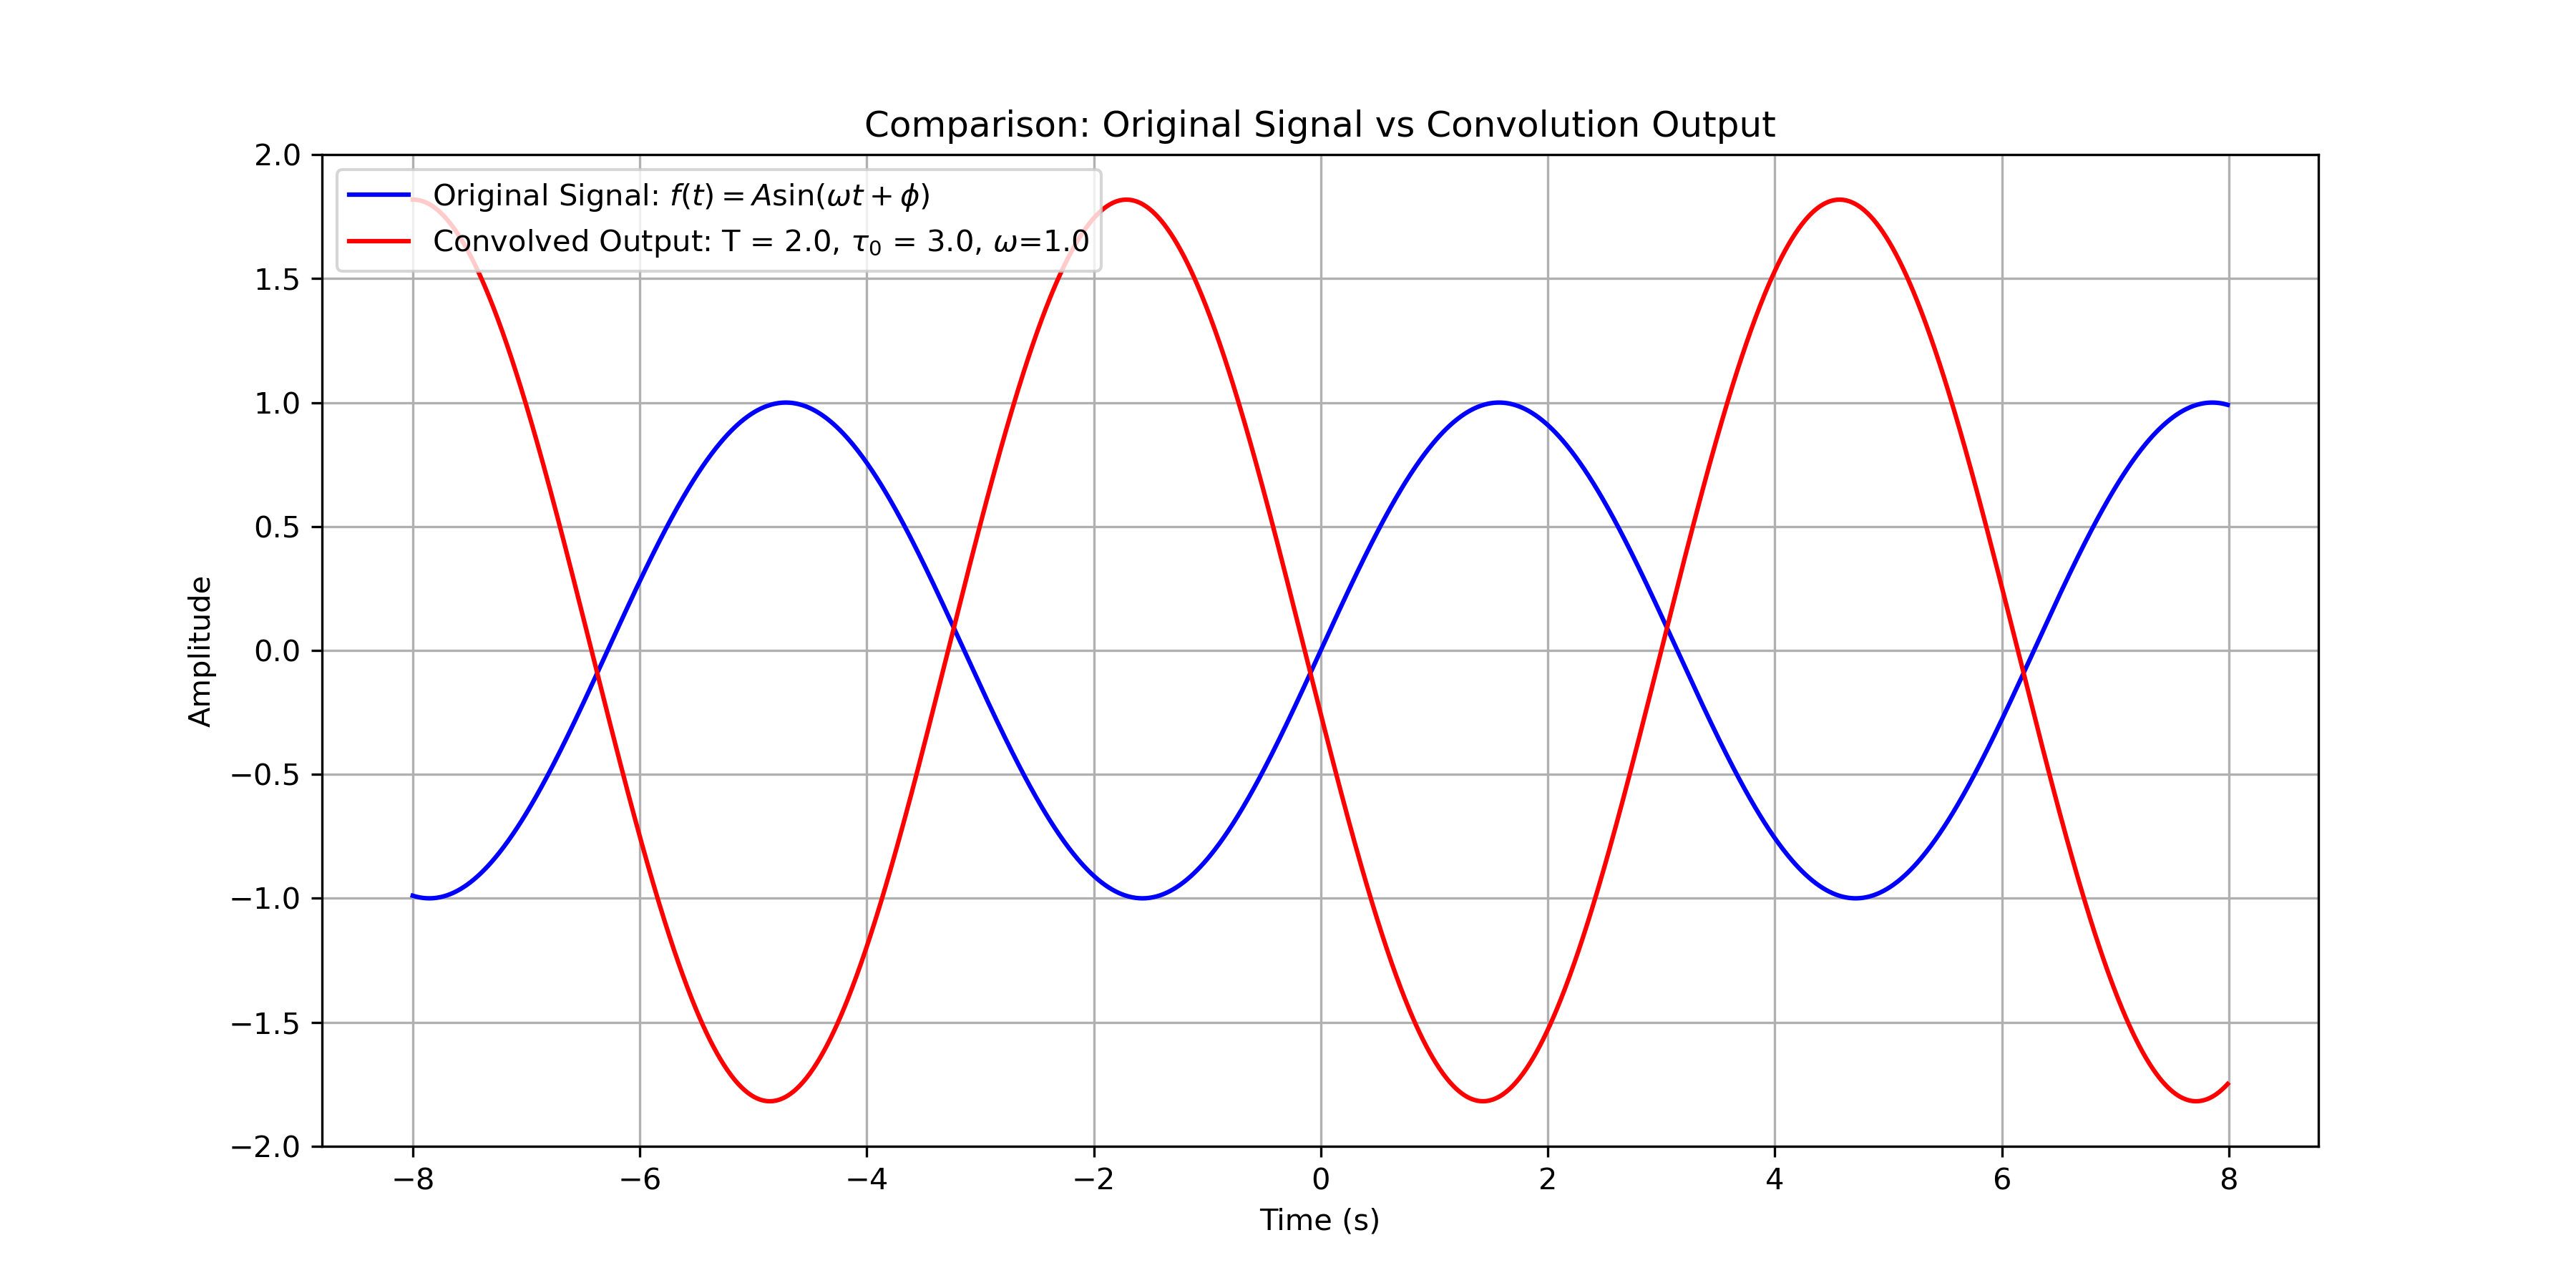
\includegraphics[width=0.95\textwidth]{codes/codes_sin_3_and_smoothening/figs/original_vs_convolved.png}
    \end{center}
    \caption{Original Signal vs Convolved Signal plot}
\end{figure}
\FloatBarrier

\subsection{Effect of Kernel Shift $\tau_0$}

The shift $\tau_0$ in the kernel results in a time delay in the output signal. This is evident from the term $\sin(\omega(t-\tau_0) + \phi)$ in our result. This demonstrates an important property of convolution: a shift in one of the functions results in an equivalent shift in the convolution result.

In the context of time-delayed systems, this shows that the system introduces a delay of $\tau_0$ in the response. This could represent physical phenomena like signal propagation delays in communication systems or processing delays in control systems.

\begin{figure}[!ht]
    \begin{center}
        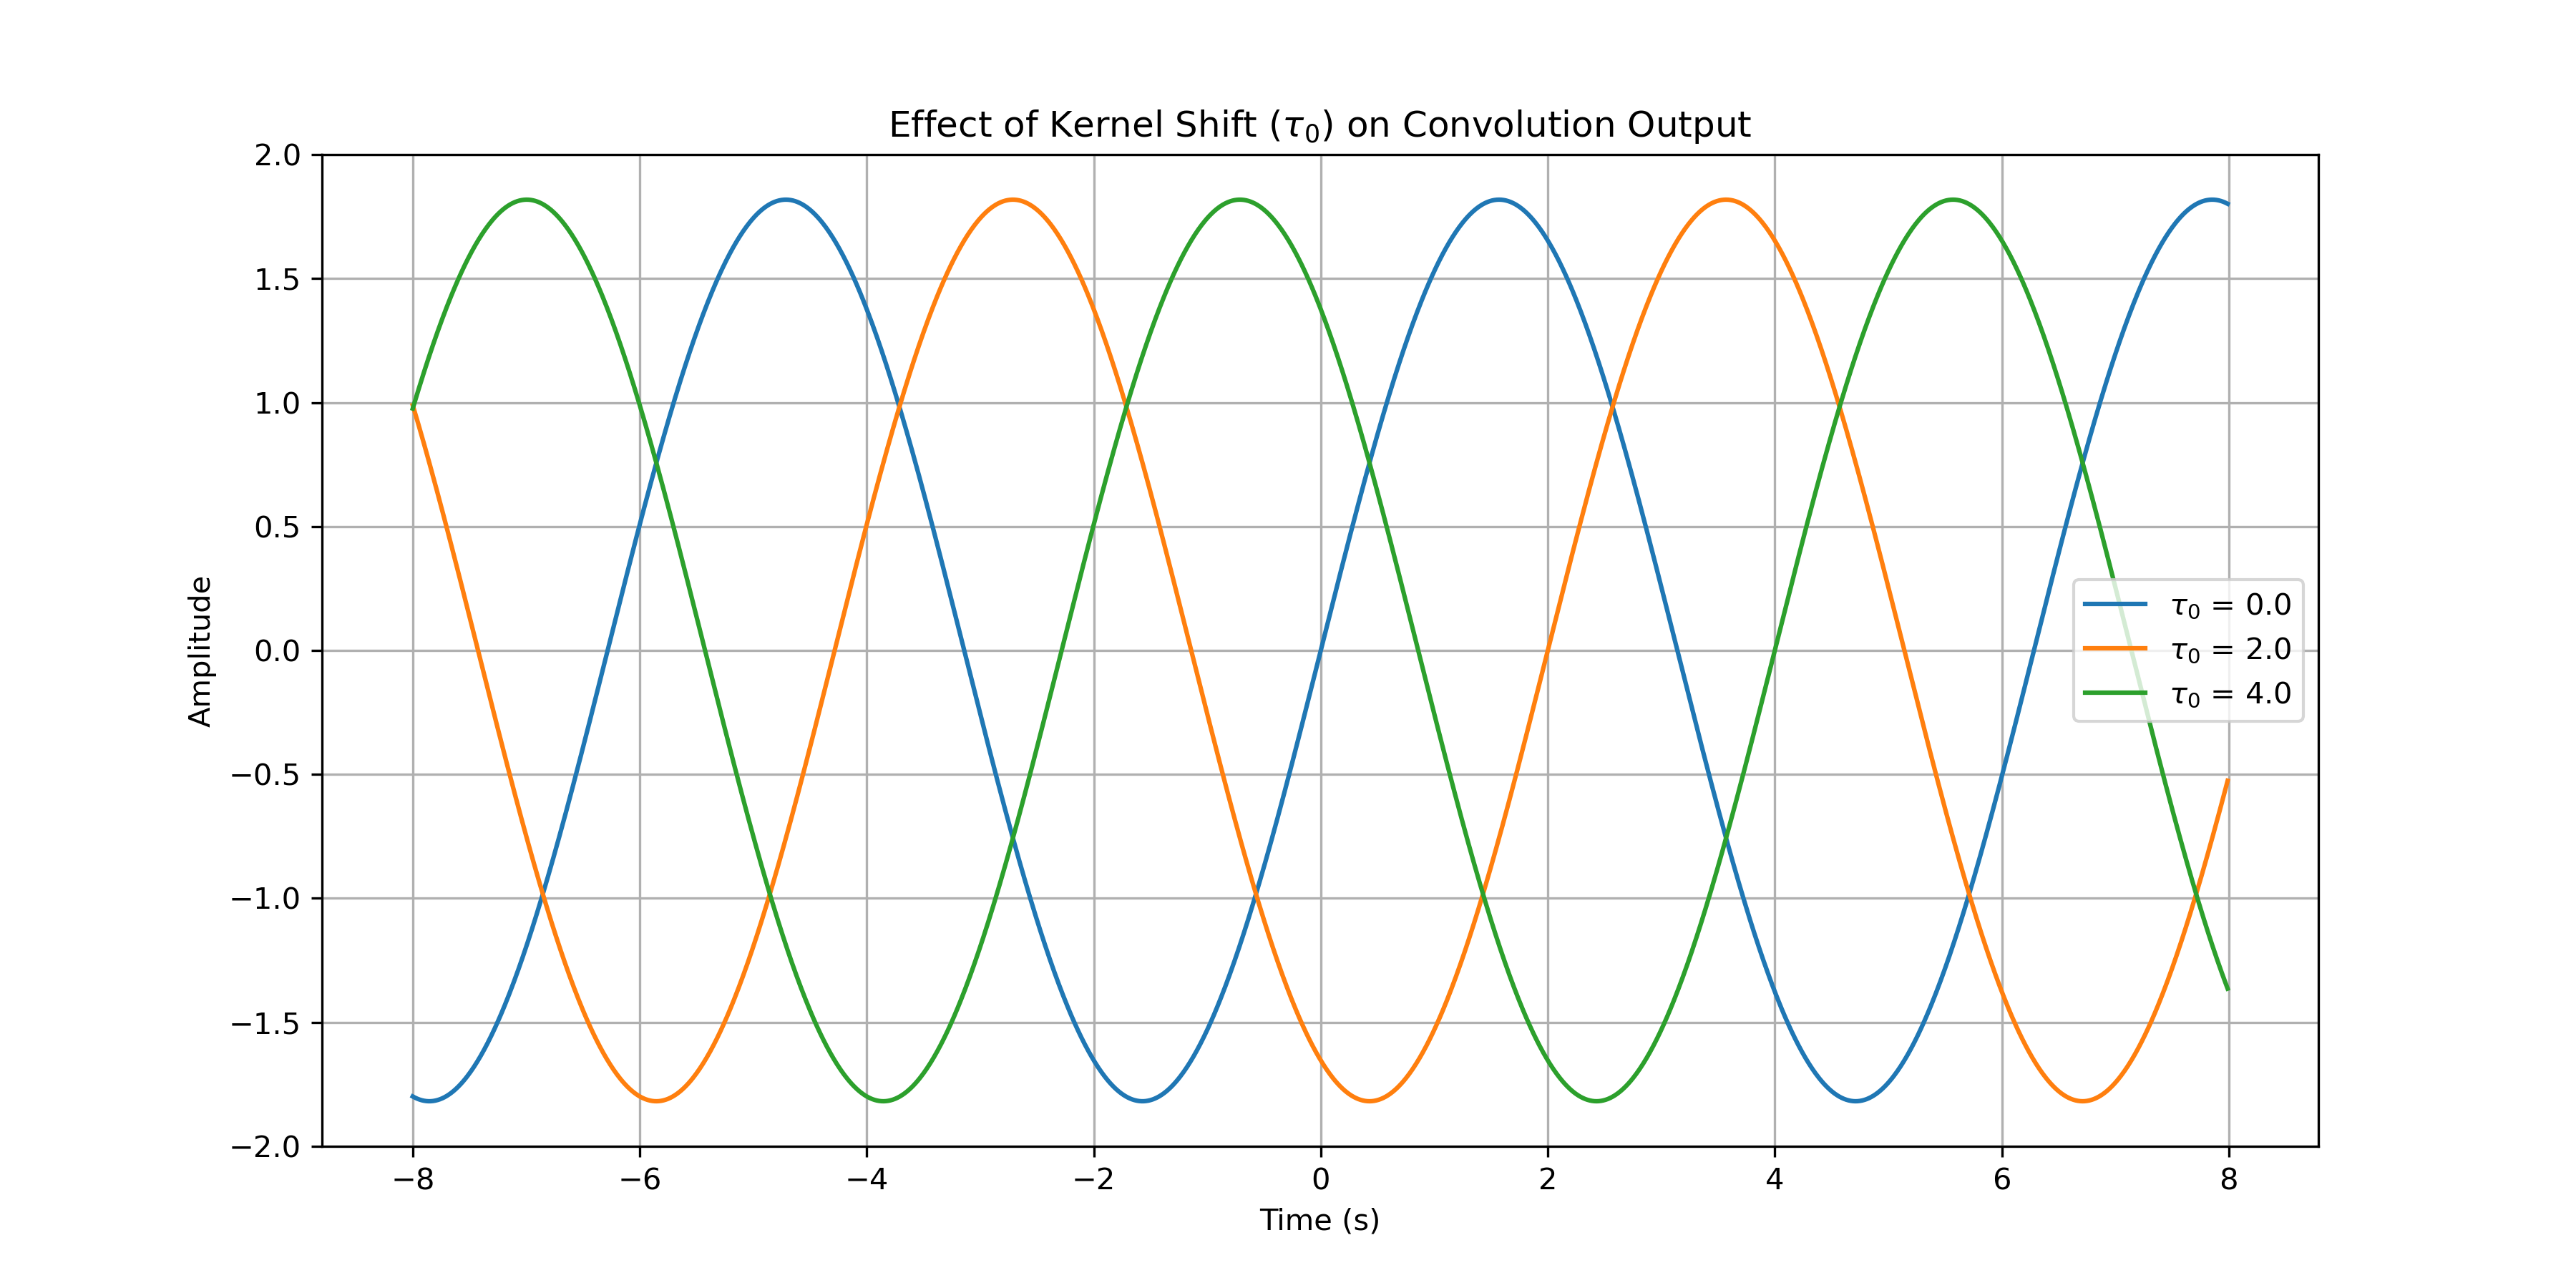
\includegraphics[width=0.95\textwidth]{codes/codes_sin_3_and_smoothening/figs/varying_tau_effect.png}
    \end{center}
    \caption{Effect of $\tau_0$ on the convoluted signal}
\end{figure}
\FloatBarrier

\subsection{Special Cases}

\begin{enumerate}
\item When $\omega T = n\pi$ (where $n$ is a non-zero integer), $\sin(\omega T) = 0$, making the output zero. This represents frequencies that are completely filtered out by the system.

\begin{figure}[!ht]
    \begin{center}
        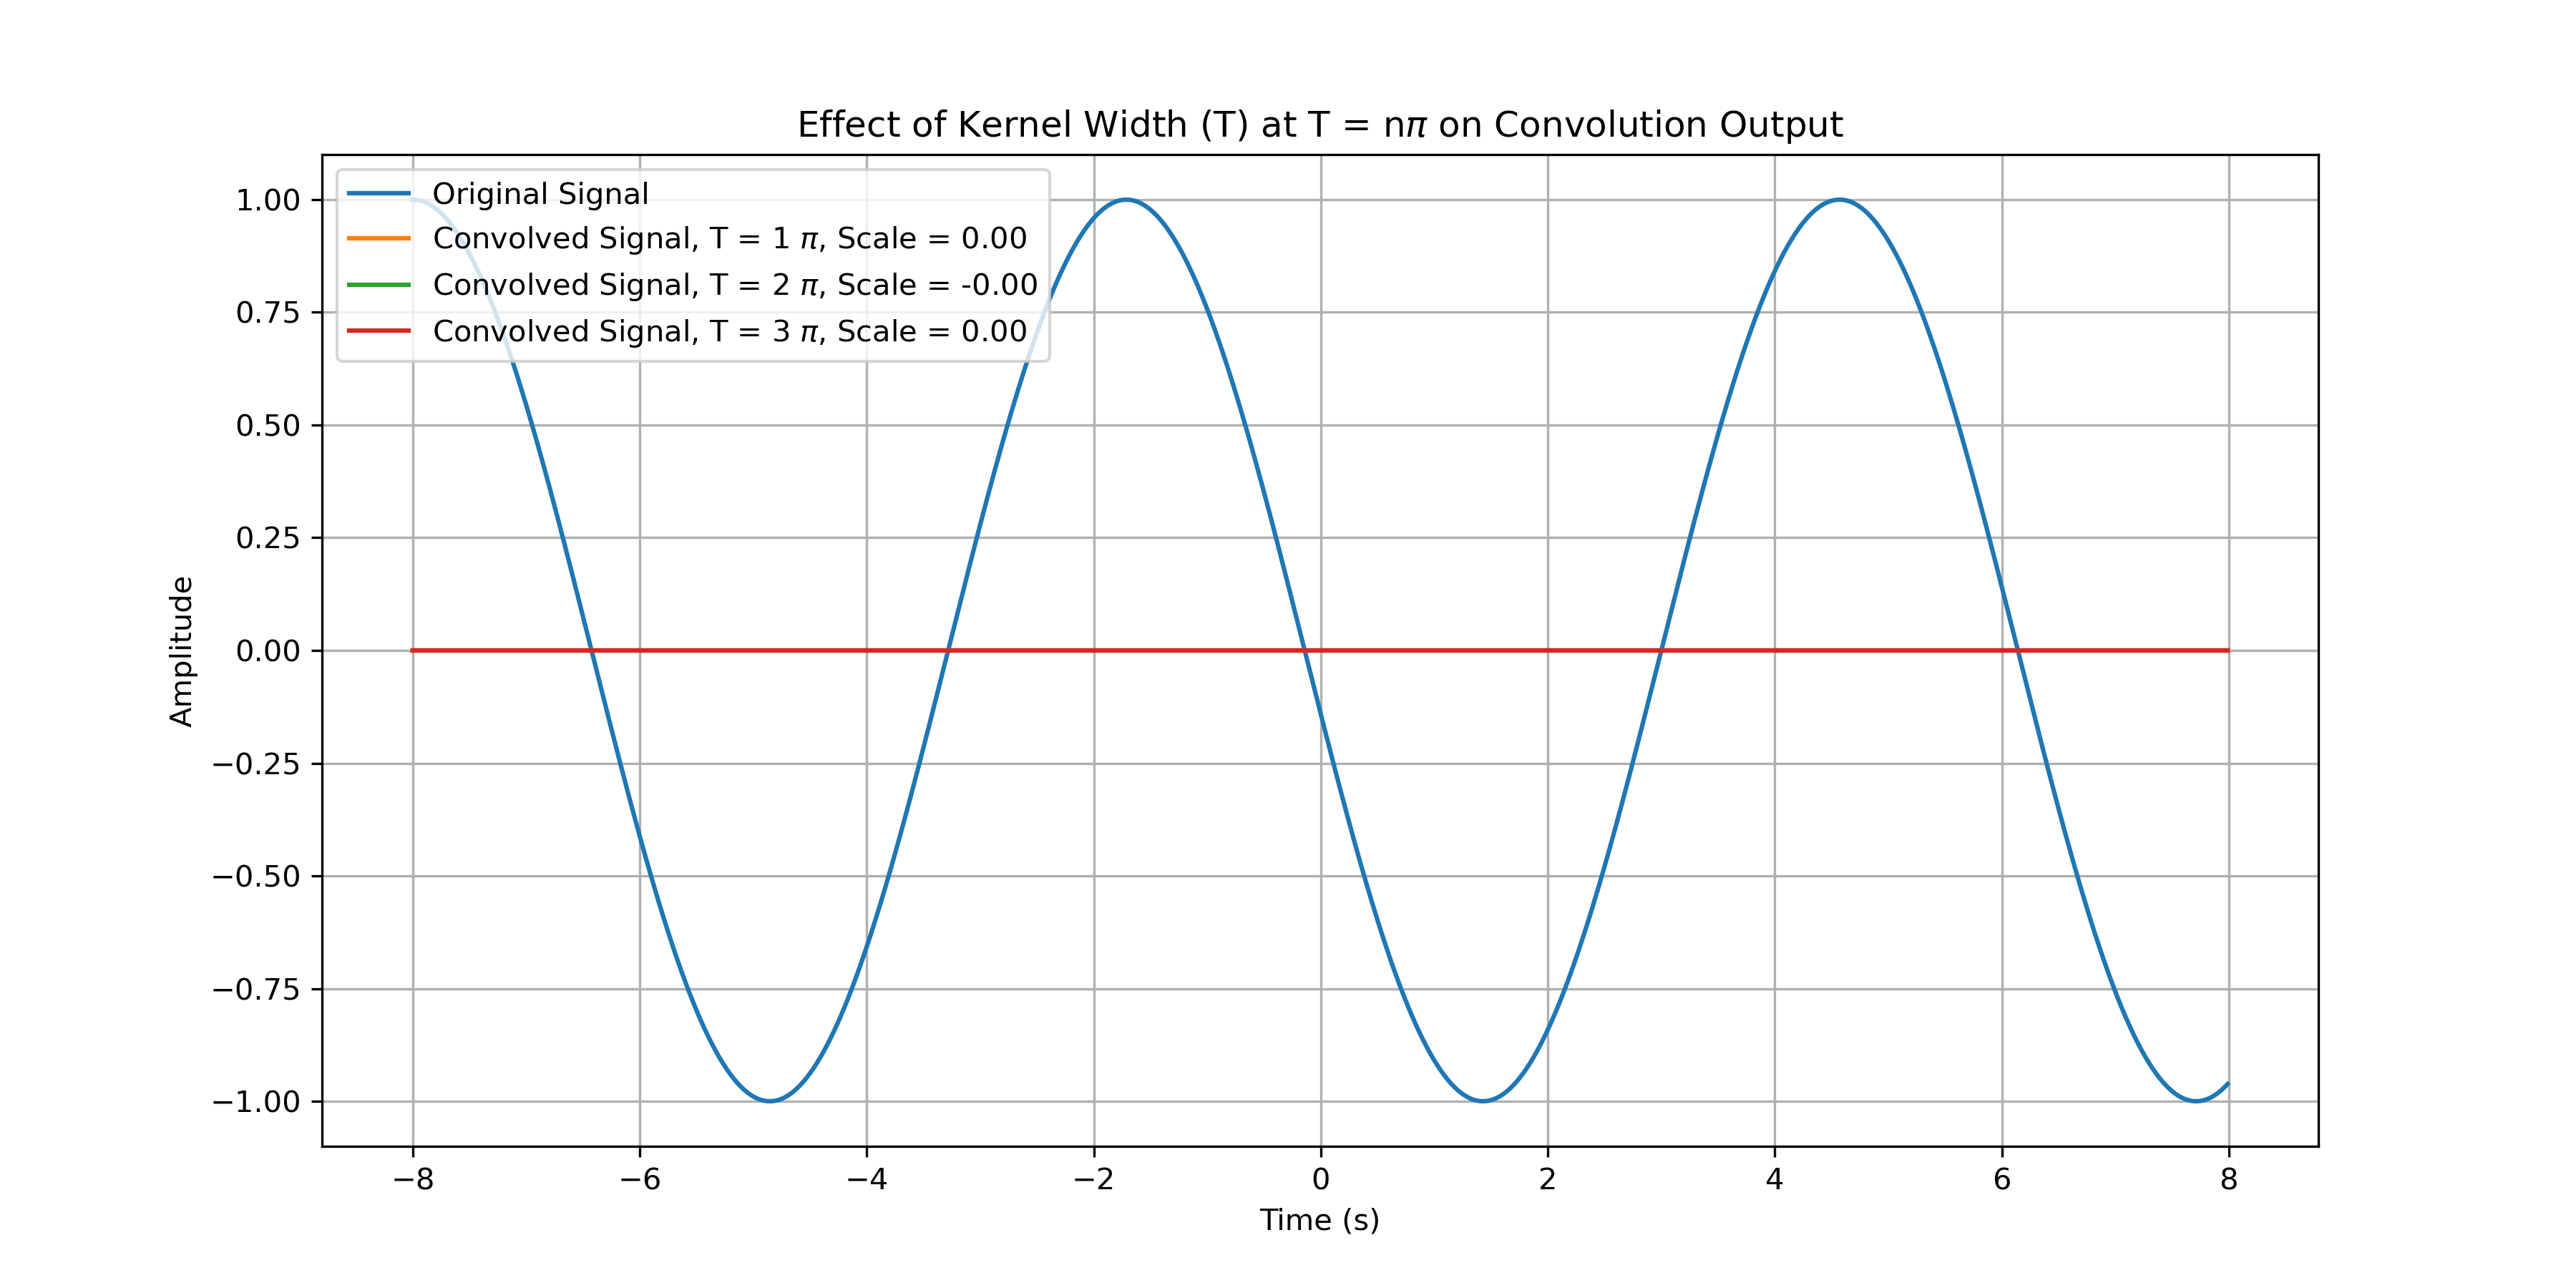
\includegraphics[width=1\textwidth]{codes/codes_sin_3_and_smoothening/figs/varying_T_pi_effect.png}
    \end{center}
\end{figure}
\FloatBarrier

\item When $T$ approaches zero, the kernel approaches a unit impulse function, and the output approaches zero for all $t$.

\item When $T$ is very large, the term $\frac{\sin(\omega T)}{\omega}$ oscillates, but its amplitude decreases as $\frac{1}{\omega}$, acting as a low-pass filter.
\end{enumerate}

\subsection{Amplitude ratio Analysis}
Amplitude ratio is given by:
\begin{align}
    \frac{A_{out}}{A_{in}} = \frac{2\sin{\omega T}}{\omega} = 2T sinc(\omega T)
\end{align}

As you can observe, it is a typical $sinc$ function which dies down as $\omega$ increases. This makes it an interesting way to filter out high frequencies, effectively making it a working but crude low-pass filter.

\begin{figure}[!ht]
    \begin{center}
        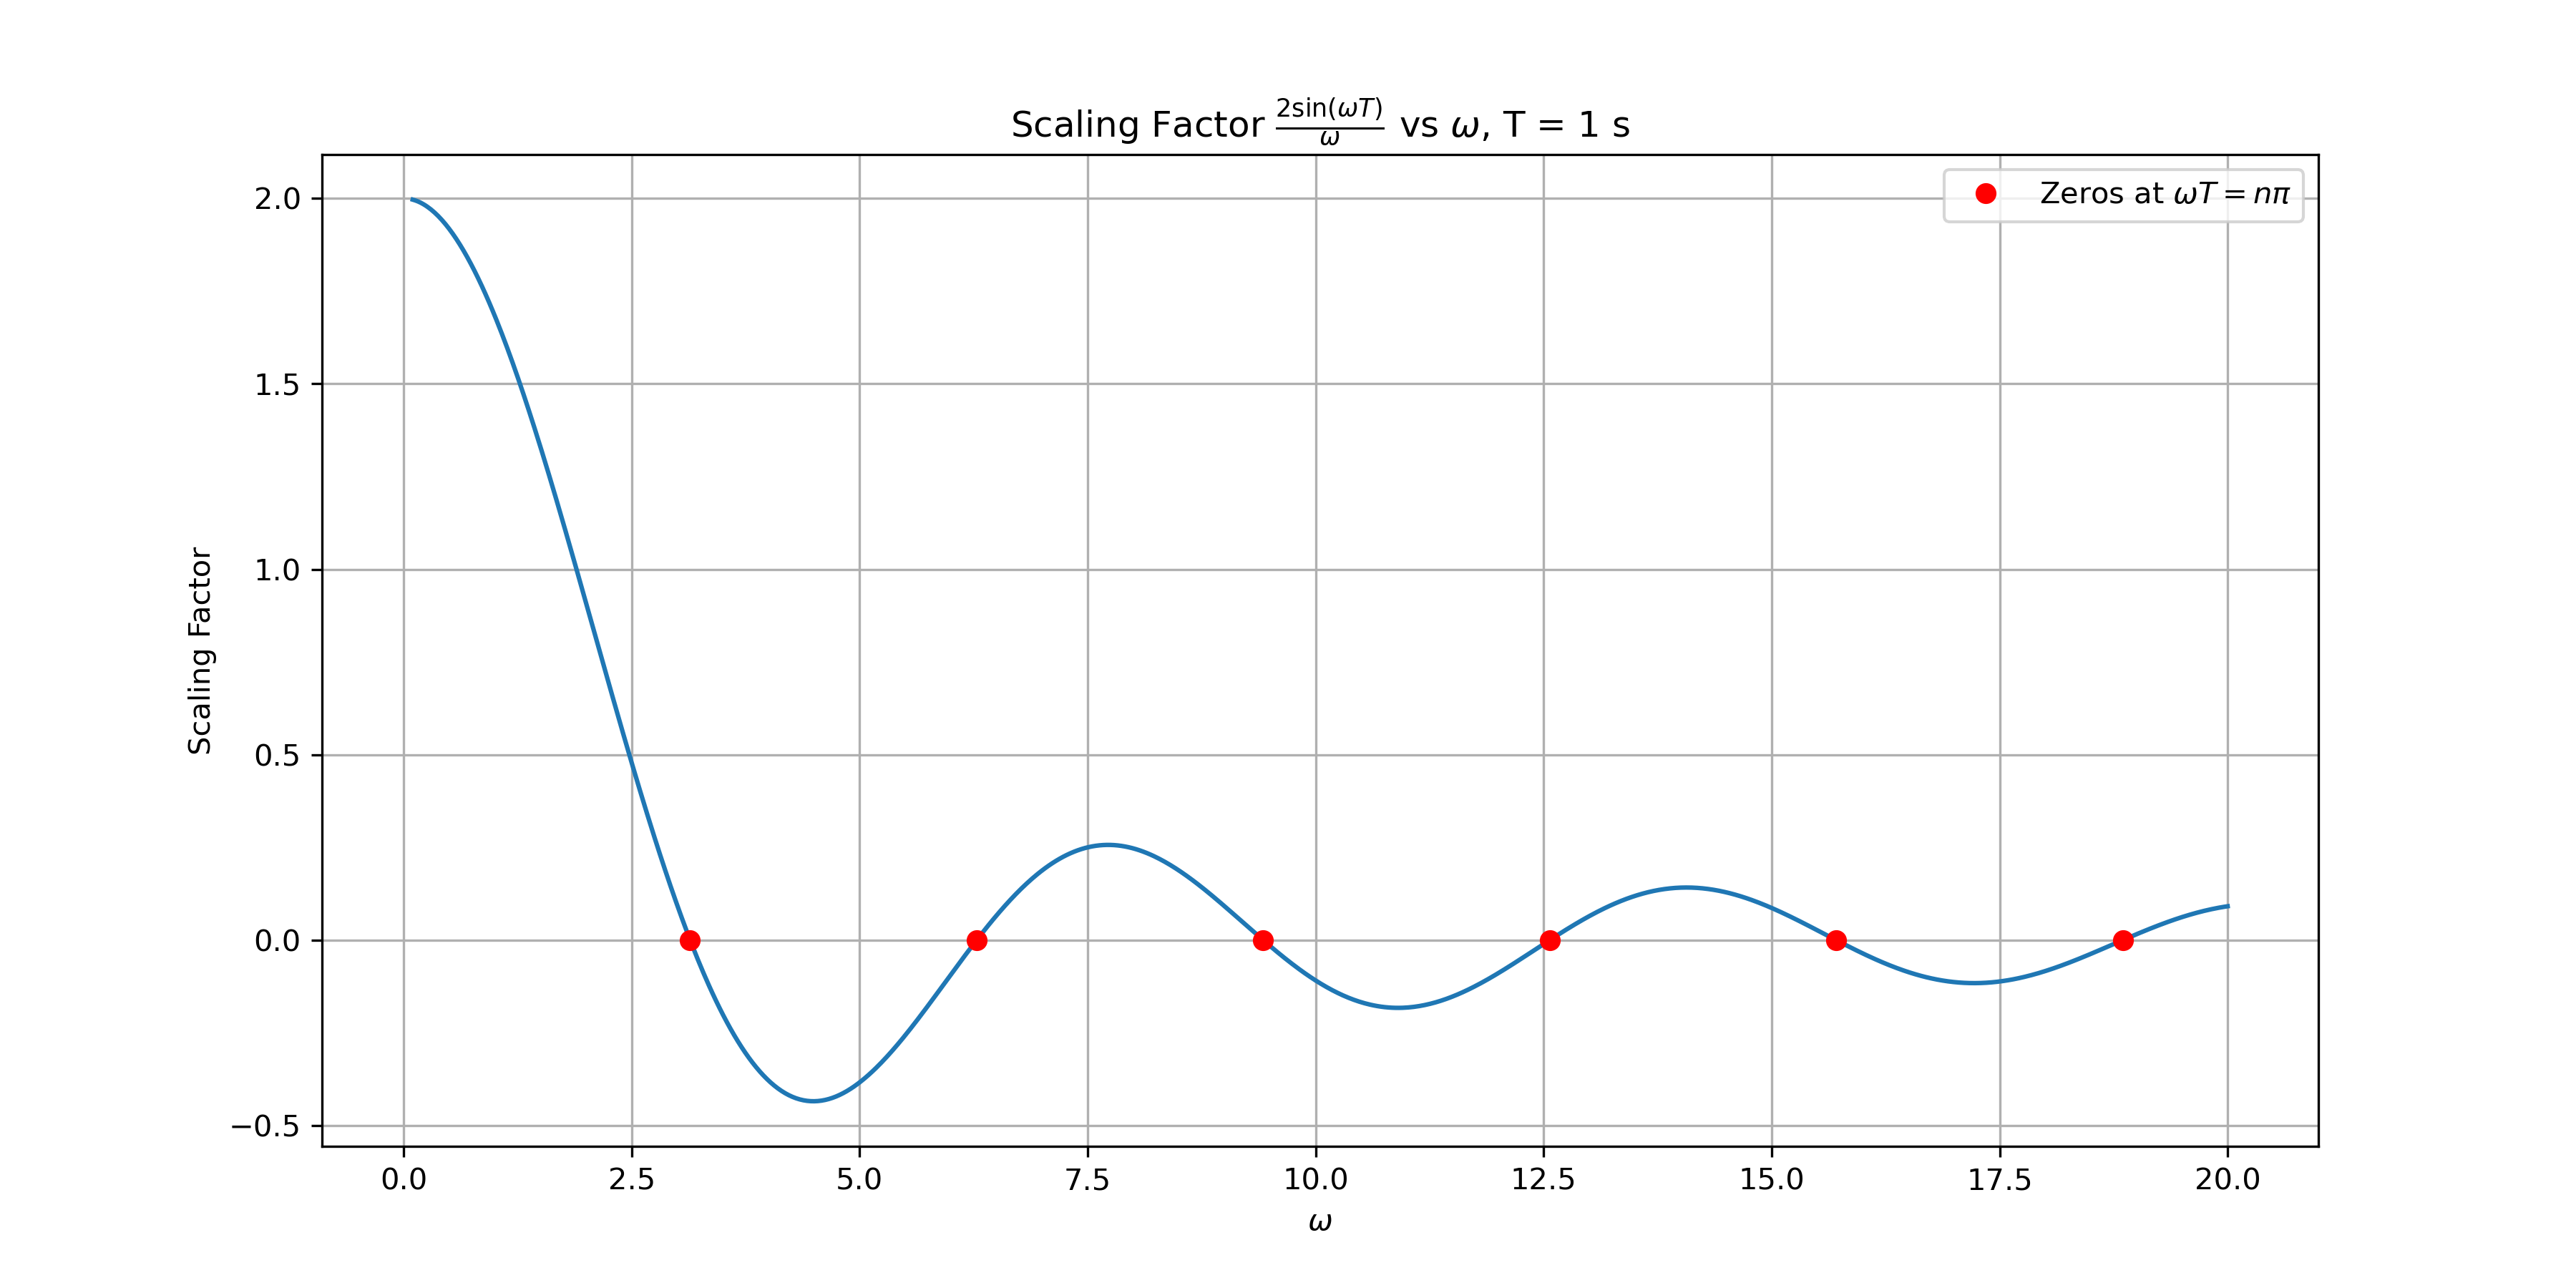
\includegraphics[width=0.95\textwidth]{codes/codes_sin_3_and_smoothening/figs/scaling_factor_analysis.png}
    \end{center}
    \caption{Amplitude/Scaling factor dependence on $\omega$ taking $T = 1s$}
\end{figure}
\FloatBarrier

The amplitude ratio is sinusoidal with respect to T with angular frequency $\omega$ when all the other parameters are constant.

\begin{figure}[!ht]
    \begin{center}
        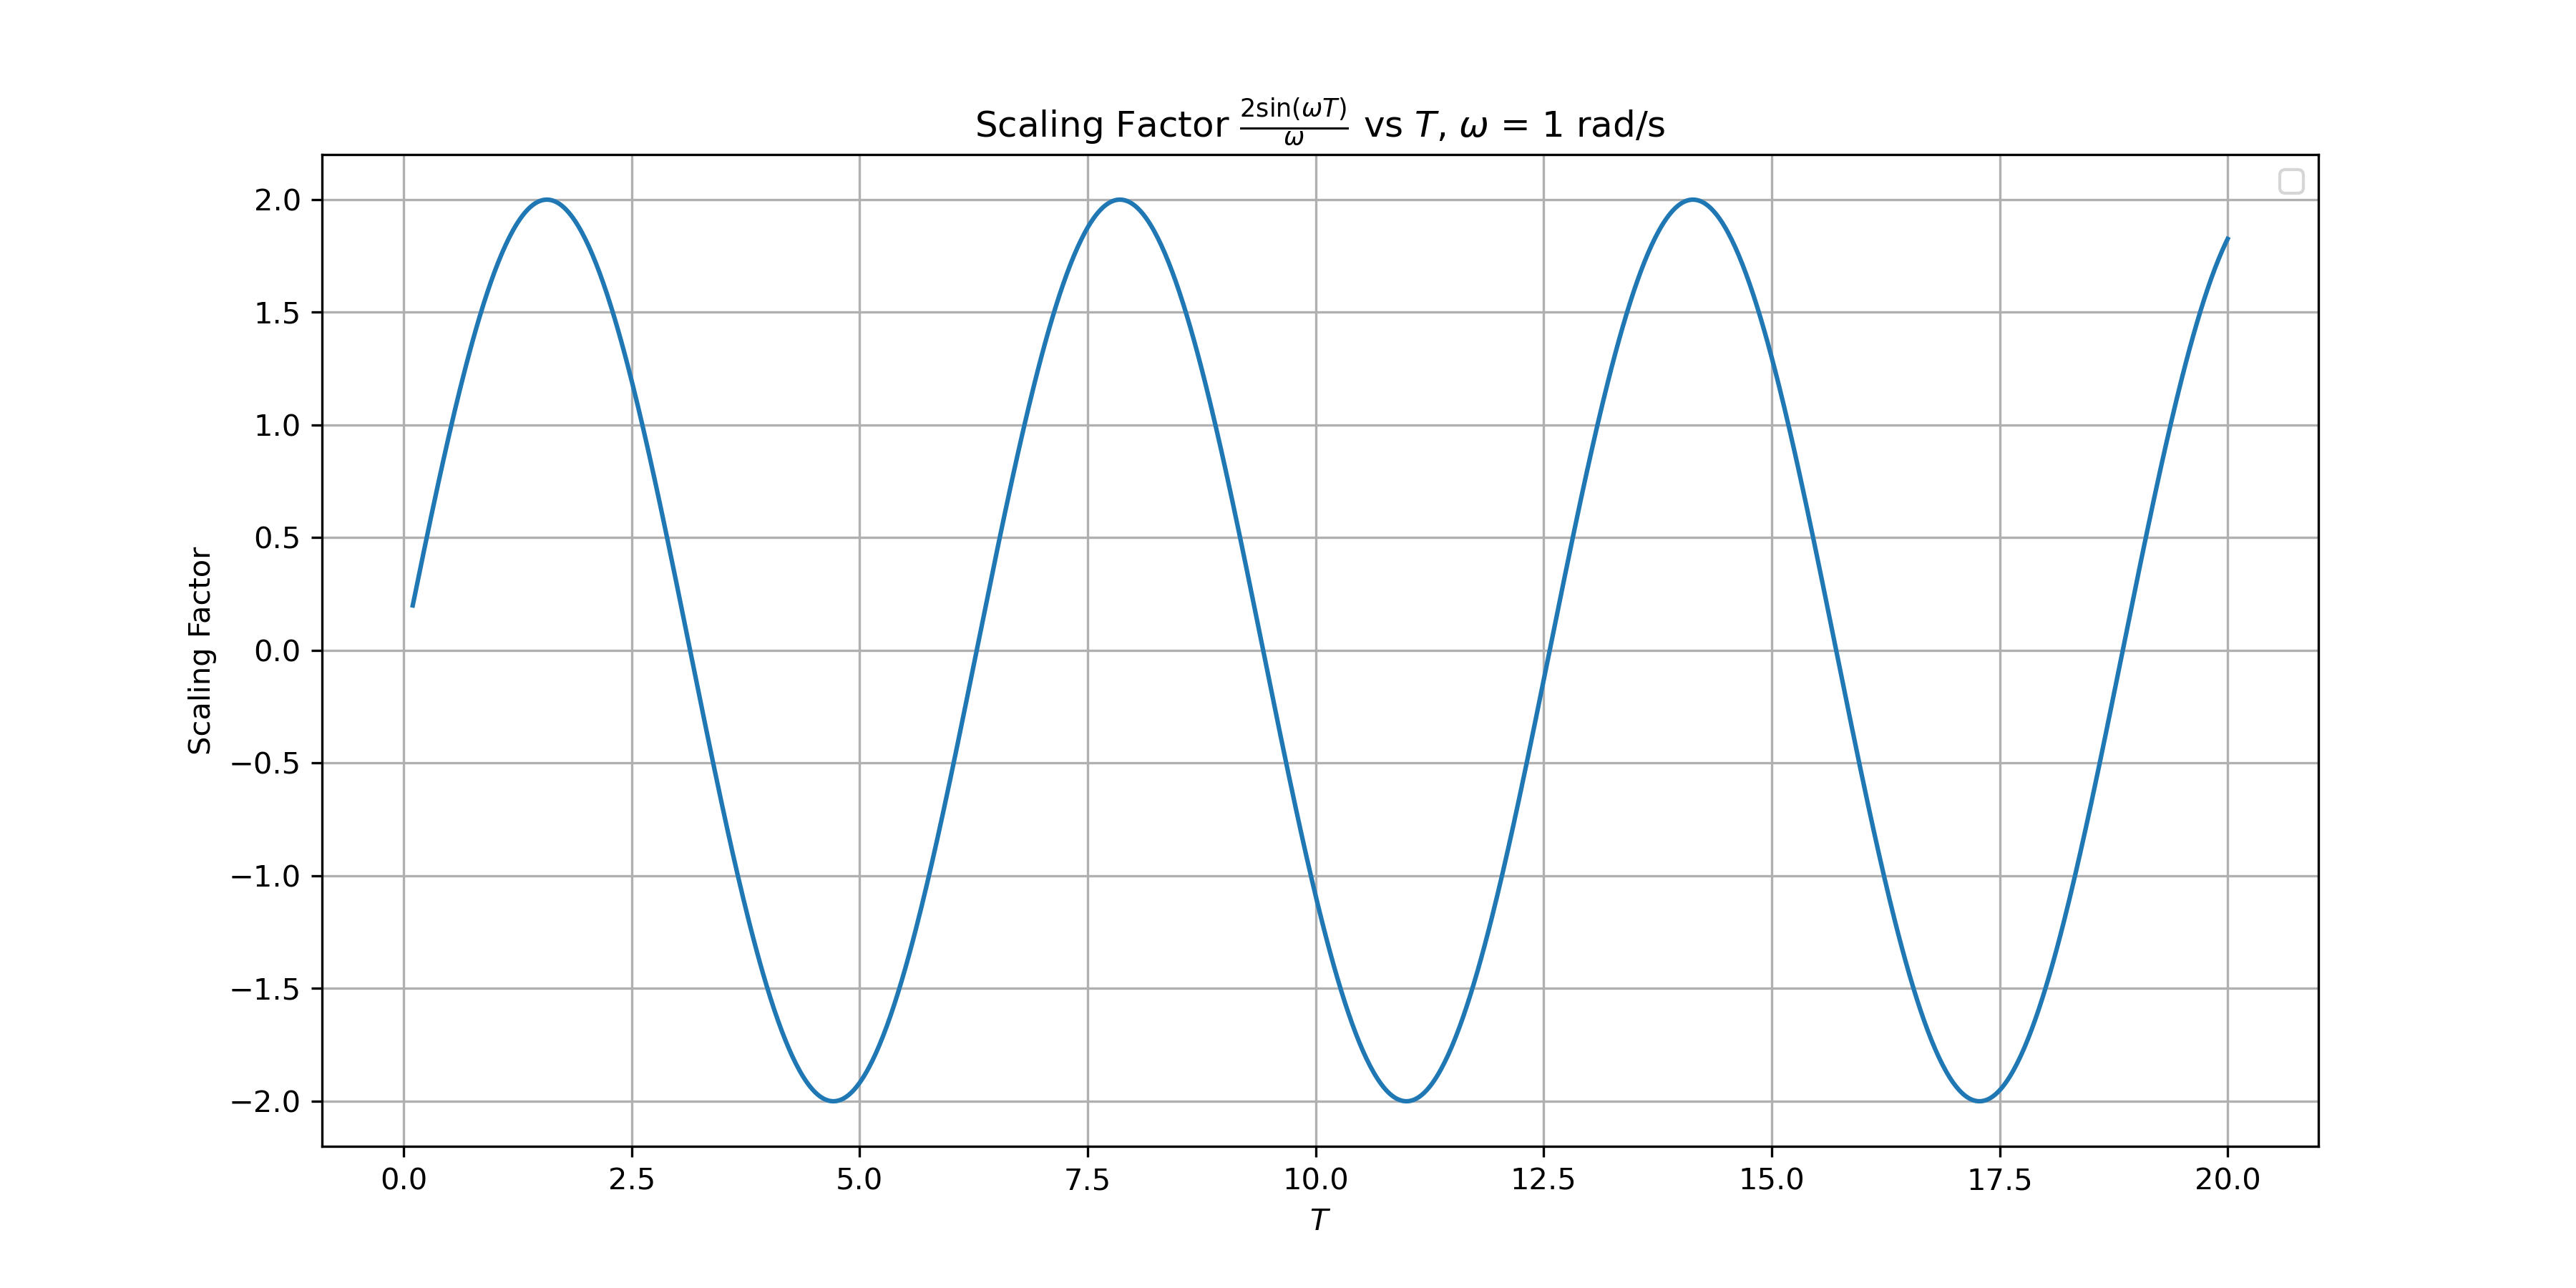
\includegraphics[width=0.95\textwidth]{codes/codes_sin_3_and_smoothening/figs/scaling_factor_analysis_T.png}
    \end{center}
    \caption{Amplitude/Scaling factor dependence on $T$ taking $w = 1 rad/s$}
\end{figure}
\FloatBarrier

\subsection{More analysis on Effect of Kernel Width (T)}
The convolved ouput's amplitude ratio is sinusoidal with respect to T when all the other parameters are constant.

\begin{figure}[!ht]
    \begin{center}
        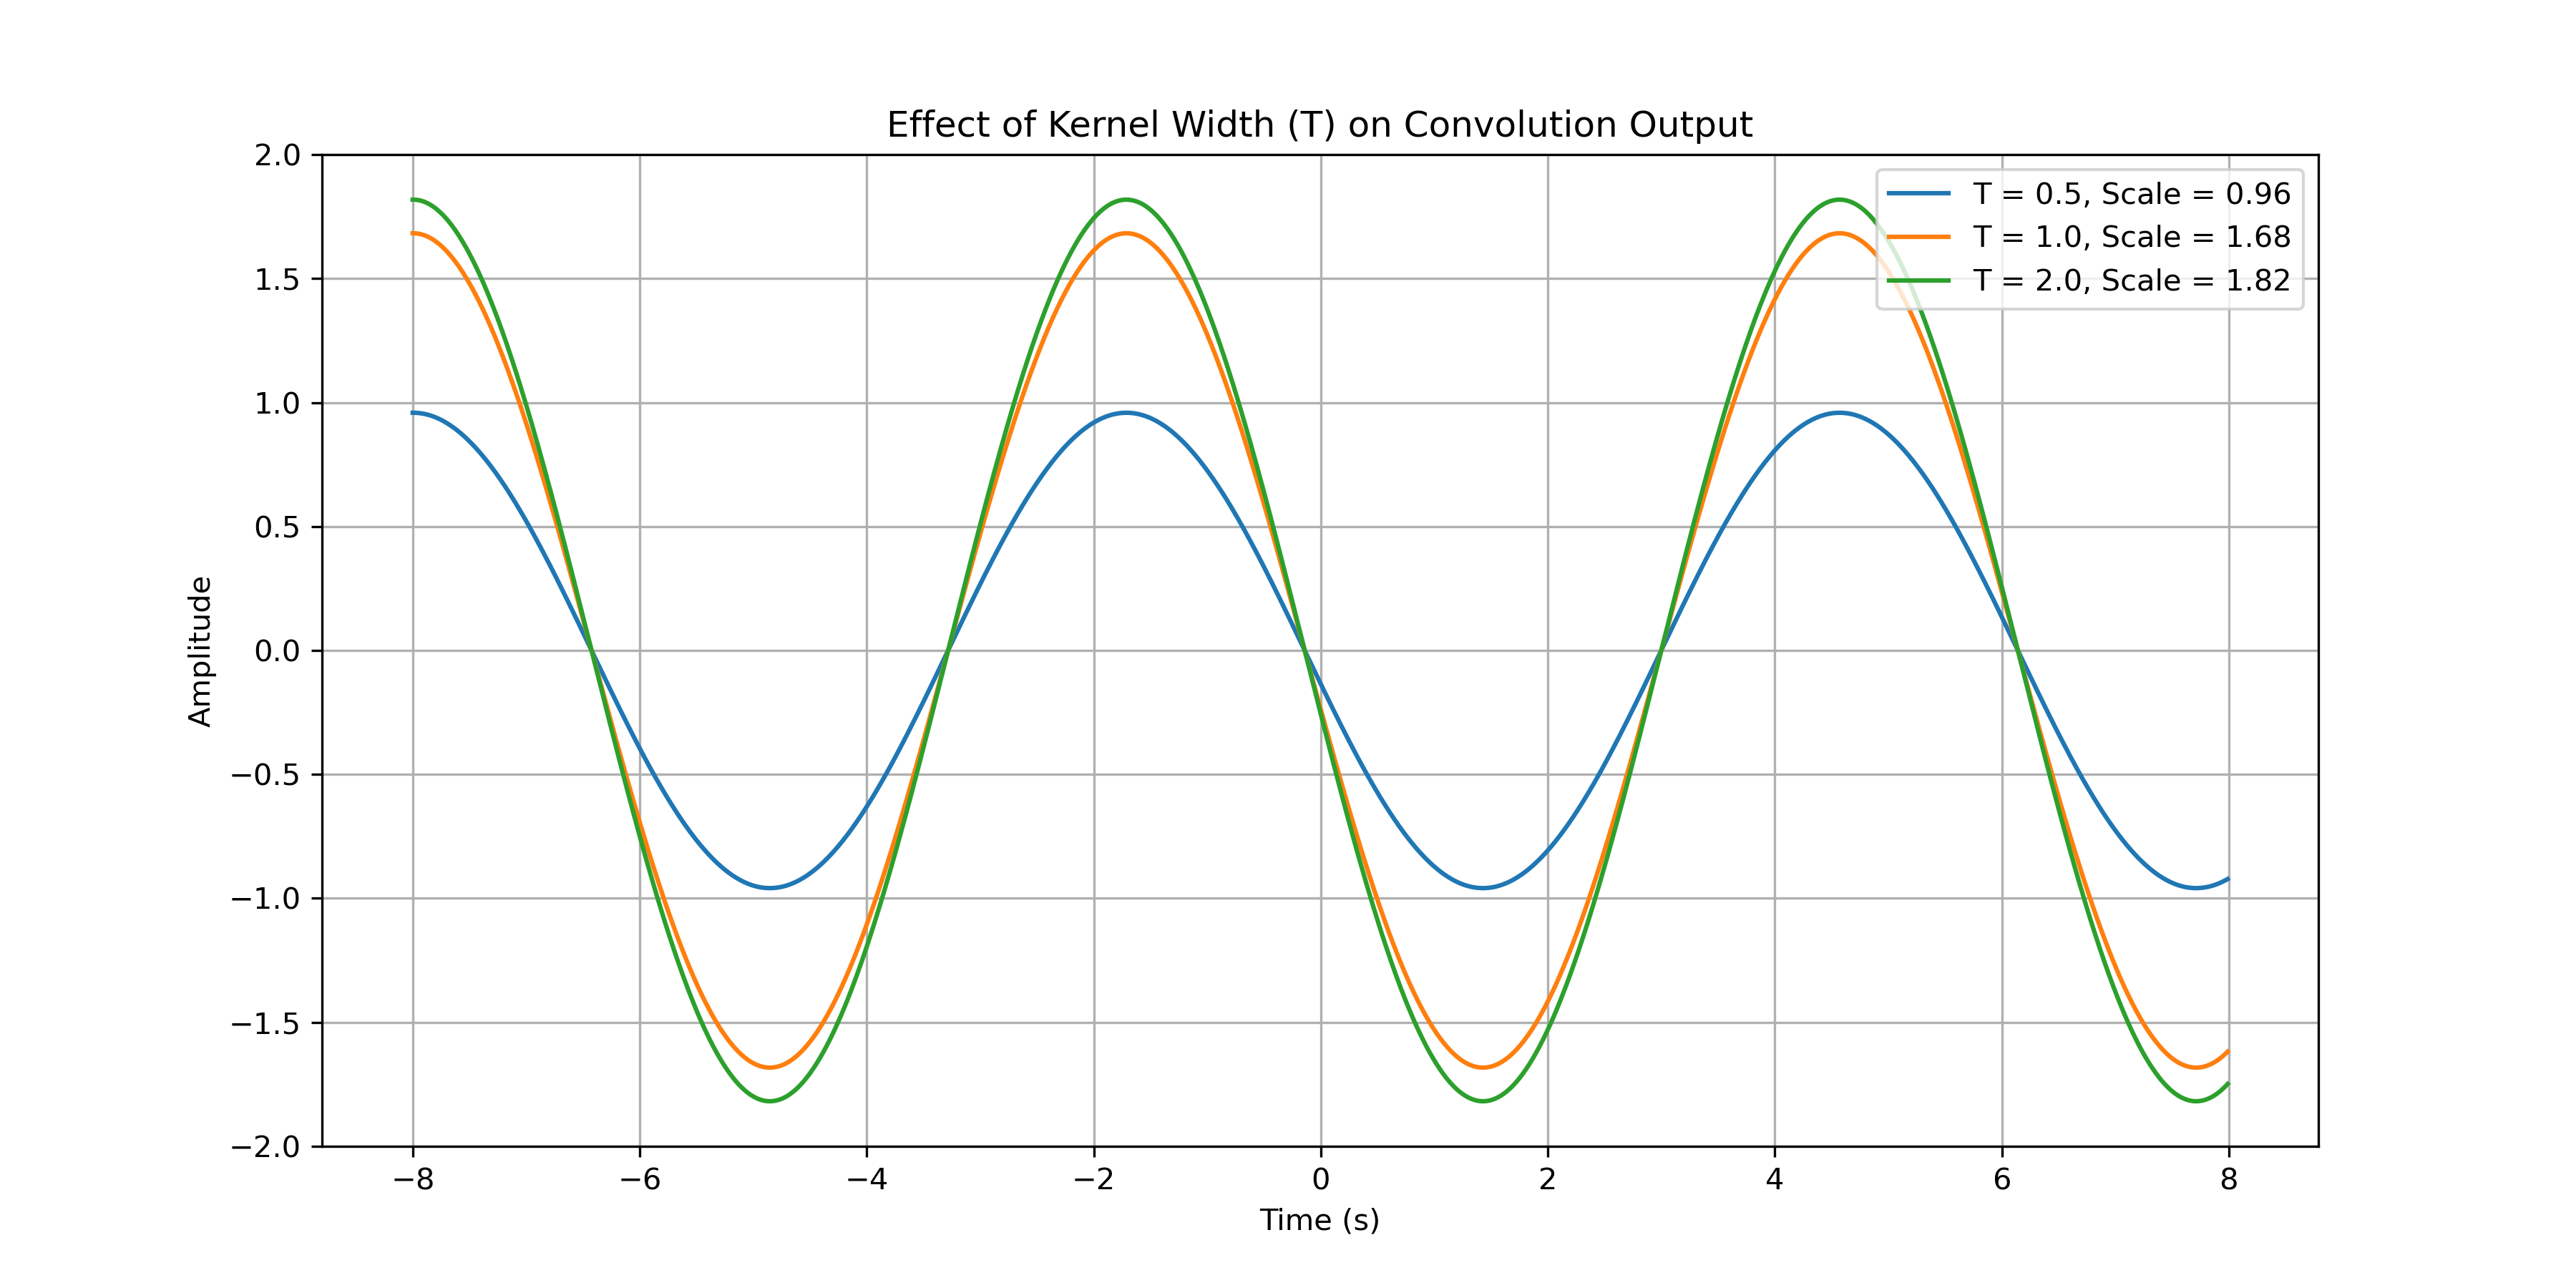
\includegraphics[width=0.95\textwidth]{codes/codes_sin_3_and_smoothening/figs/varying_T_effect.png}
    \end{center}
    \caption{Effect of Varying T on the Convolved output}
\end{figure}
\FloatBarrier

\section{Inverse Sinusoidal as $f(t)$}
This report analyzes the convolution of the inverse sine function with a rectangular kernel, examining both analytical and numerical approaches. We investigate how system parameters influence the convolution output while addressing the unique challenges posed by the arcsin function's domain constraints and singularities.

\subsection{Mathematical Formulation}

\subsubsection{Convolution Definition}
The convolution of an input signal $f(t)$ with a kernel $h(t)$ is defined as:
\begin{equation}
y(t) = (f * h)(t) = \int_{-\infty}^{\infty} f(\tau)h(t-\tau)d\tau
\end{equation}

For our specific case:
\begin{align}
f(t) &= 
\begin{cases}
A\arcsin(t), & -1 \leq t \leq 1 \\
0, & \text{otherwise}
\end{cases} \\
h(t) &= 
\begin{cases} 
1, & |t| \leq T \\
0, & \text{otherwise}
\end{cases}
\end{align}

\subsubsection{Analytical Solution}
The convolution integral becomes:
\begin{equation}
y(t) = \int_{t-T}^{t+T} A\arcsin(\tau)d\tau
\end{equation}

Using the primitive $\int \arcsin(x)dx = x\arcsin(x) + \sqrt{1-x^2} + C$, we derive the piecewise solution:

\begin{align*}
y(t) &= \begin{cases}
A\left[(t+T)\arcsin(t+T) + \sqrt{1-(t+T)^2}\right. \\
\quad \left.- (t-T)\arcsin(t-T) - \sqrt{1-(t-T)^2}\right], & \text{Case 1: } -1 \leq t-T \leq t+T \leq 1 \\
A\left[(t+T)\arcsin(t+T) + \sqrt{1-(t+T)^2} + \frac{\pi}{2}\right], & \text{Case 2: } t-T < -1 \leq t+T \leq 1 \\
A\left[\frac{\pi}{2} - (t-T)\arcsin(t-T) - \sqrt{1-(t-T)^2}\right], & \text{Case 3: } -1 \leq t-T \leq 1 < t+T \\
A\pi, & \text{Case 4: } t-T < -1 \text{ and } t+T > 1
\end{cases}
\end{align*}

\subsection{Numerical Implementation}
The numerical approach discretizes the convolution integral:
\begin{equation}
y[n] = \Delta t \sum_{k=-N}^{N} f[k]h[n-k]
\end{equation}

Key considerations:
\begin{itemize}
\item Strict domain enforcement for the arcsin function
\item Proper handling of integration limits at domain boundaries
\item Special handling of boundary regions
\end{itemize}

\begin{figure}[H]
    \centering
    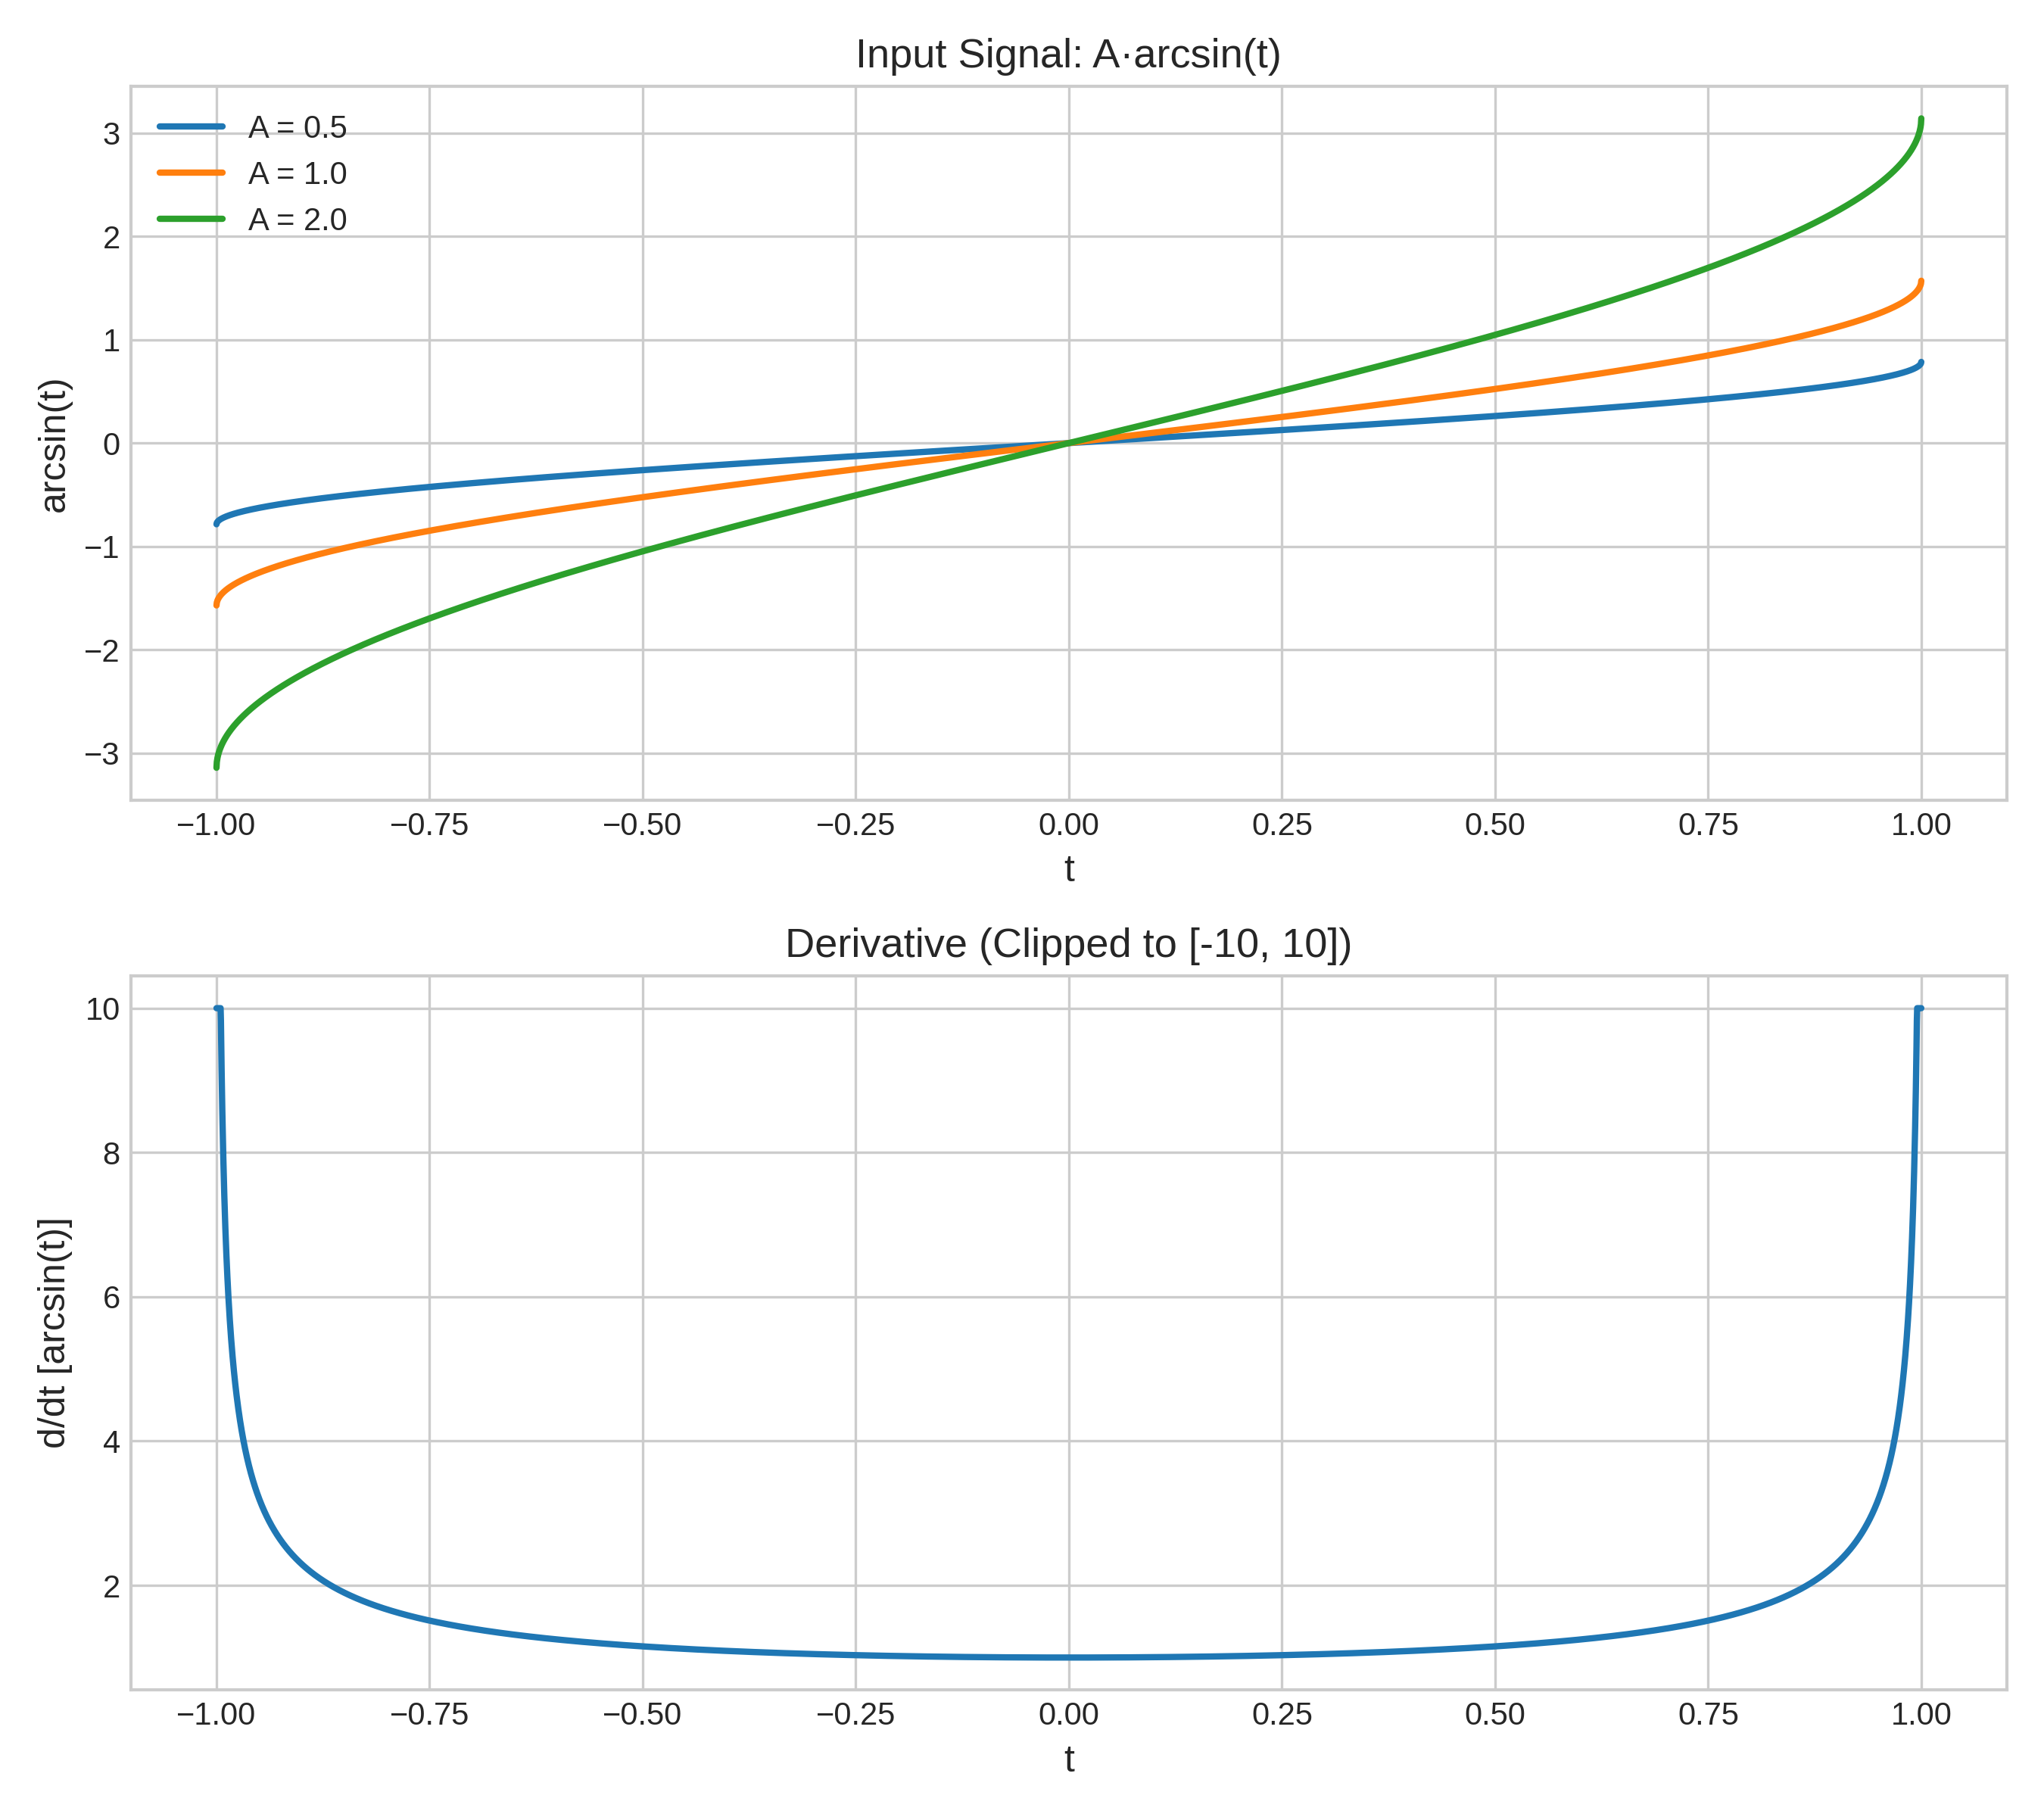
\includegraphics[width=0.85\textwidth]{codes/codes_sin_1_and_arcsin/figures/arcsin_properties.png}
    \caption{Properties of the arcsin function showing (a) amplitude variations and (b) singular derivative at boundaries}
    \label{fig:properties}
\end{figure}

\subsection{Parameter Analysis}

\subsubsection{Amplitude Effects}
\begin{figure}[H]
    \centering
    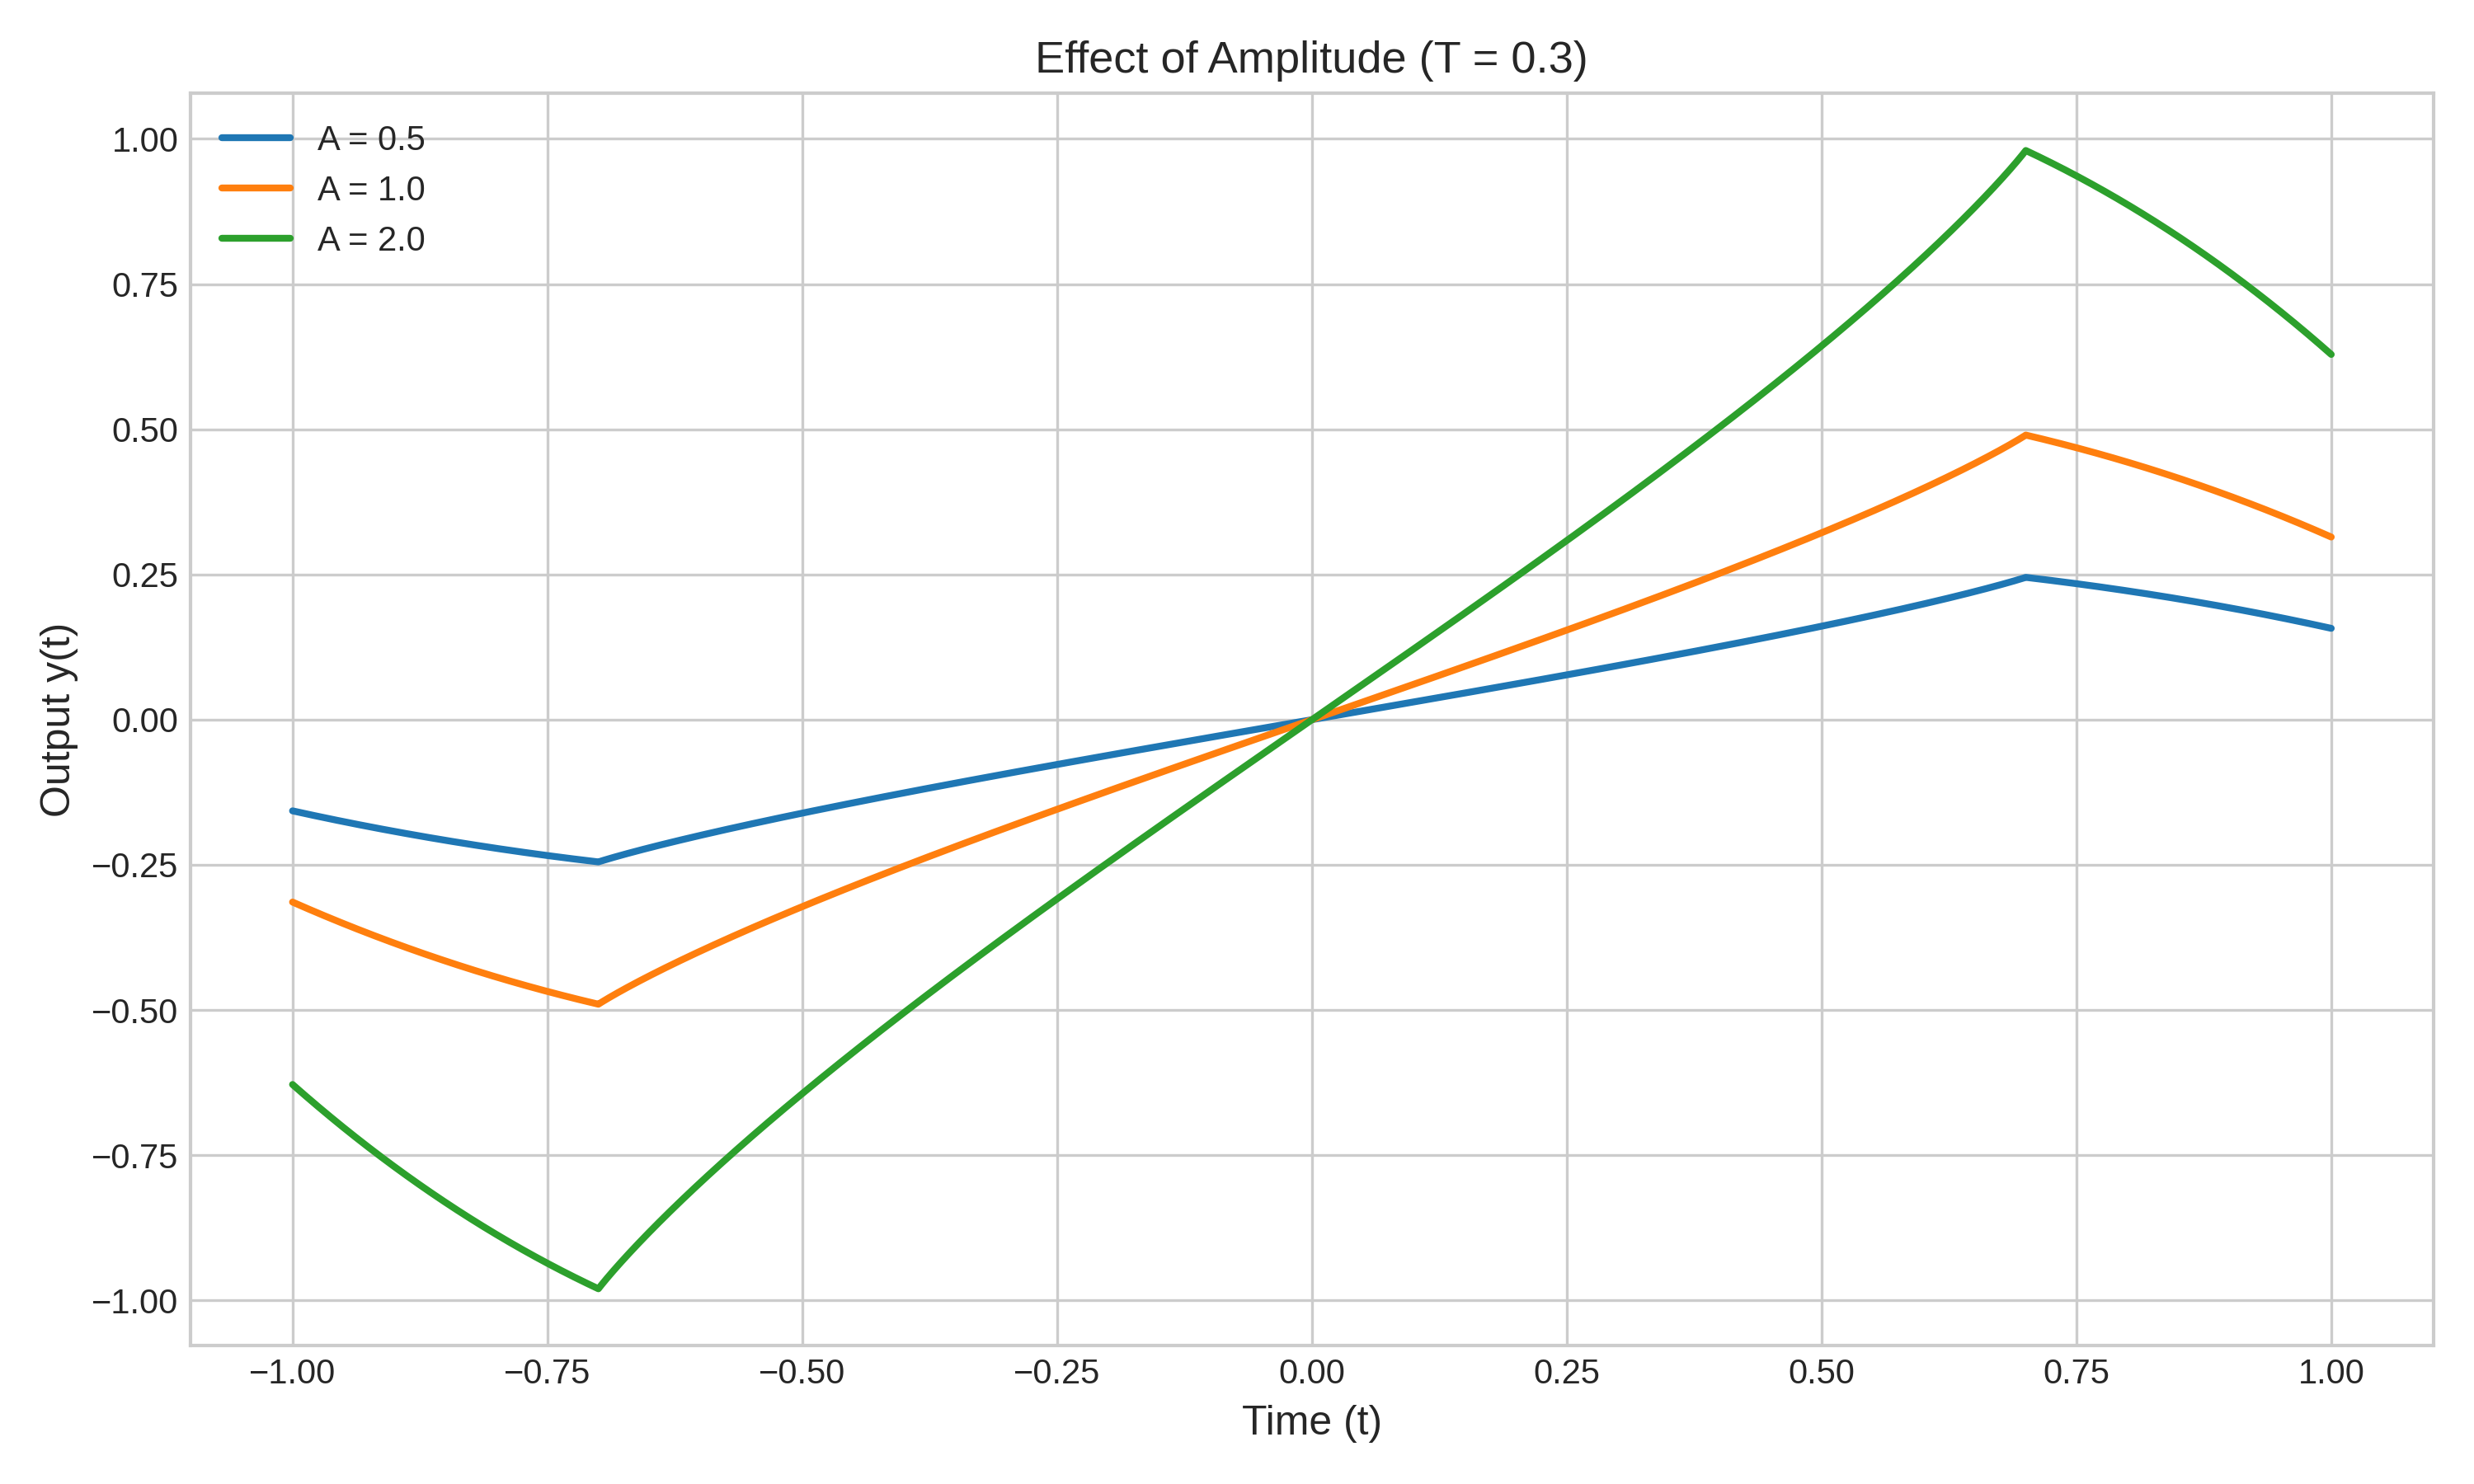
\includegraphics[width=0.85\textwidth]{codes/codes_sin_1_and_arcsin/figures/amplitude_effect.png}
    \caption{Linear scaling of convolution output with amplitude $A$ (kernel width $T=0.3$)}
    \label{fig:amplitude}
\end{figure}

Key observations:
\begin{itemize}
\item Output amplitude scales linearly with $A$
\item Shape preservation demonstrates system linearity
\item Boundary effects remain consistent across amplitudes
\end{itemize}

\subsubsection{Kernel Width Effects}
\begin{figure}[H]
    \centering
    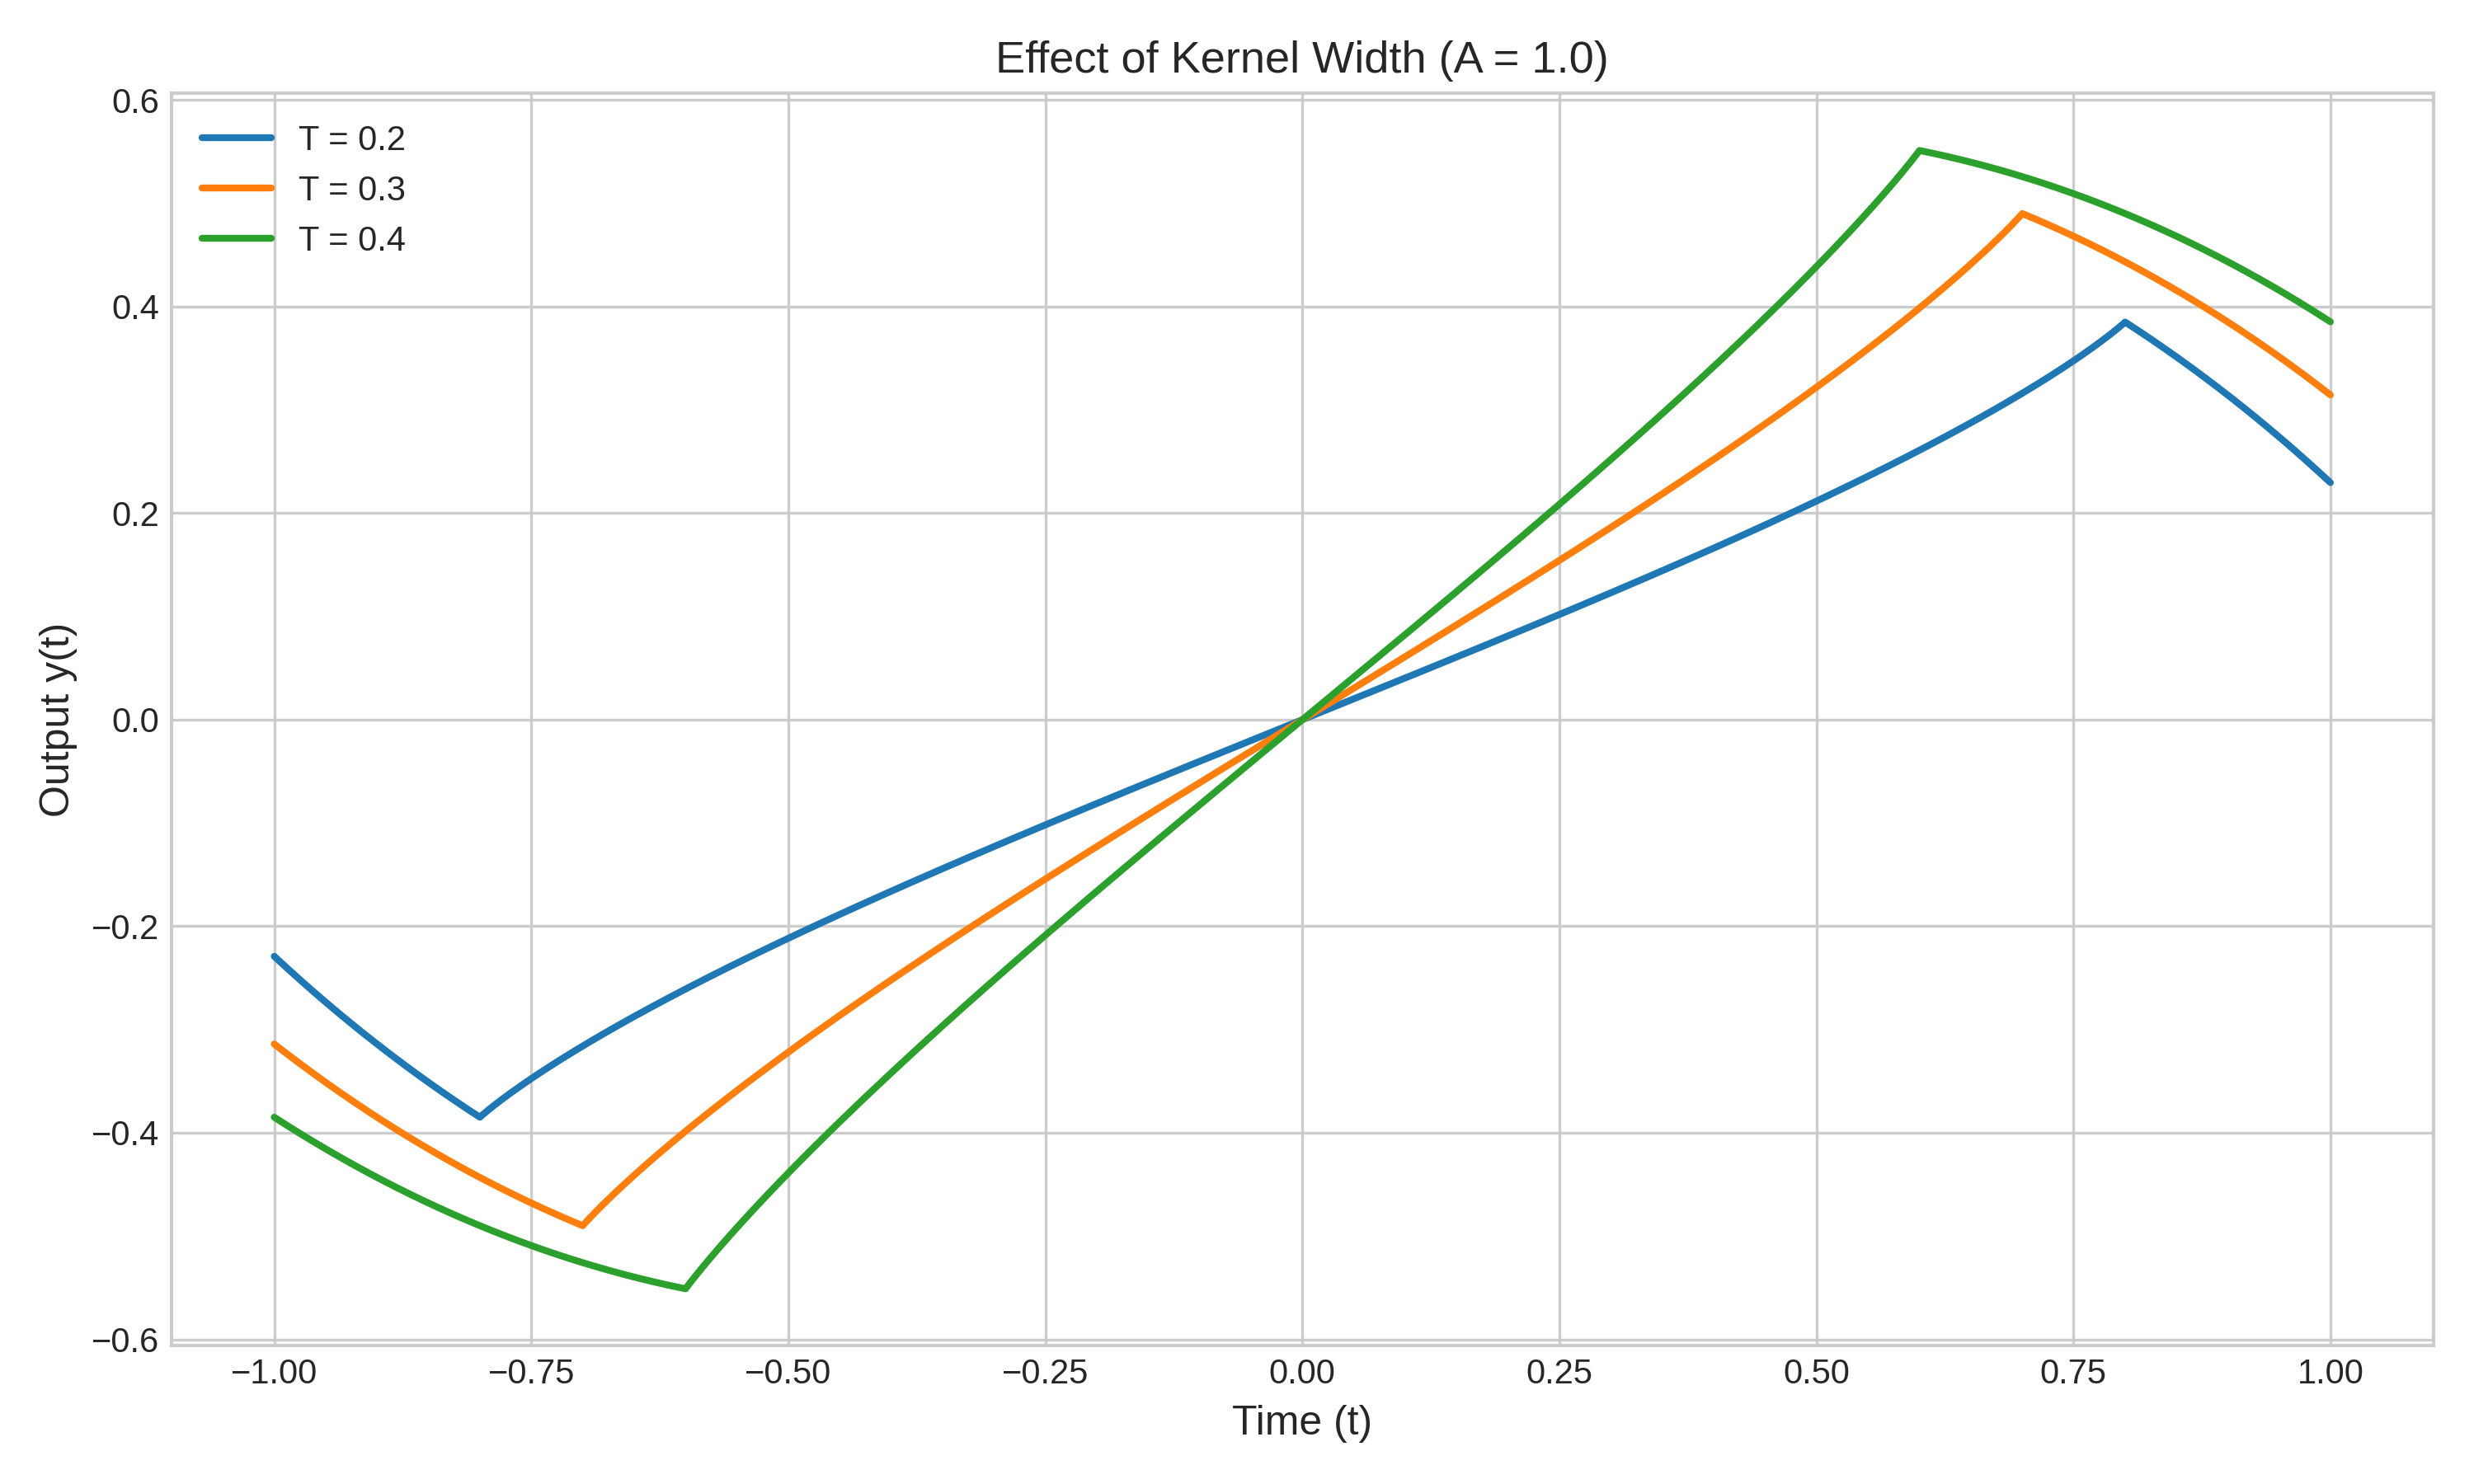
\includegraphics[width=0.85\textwidth]{codes/codes_sin_1_and_arcsin/figures/kernel_width_effect.png}
    \caption{Impact of kernel width $T$ on output smoothing (amplitude $A=1$)}
    \label{fig:kernel}
\end{figure}

Key observations:
\begin{itemize}
\item Wider kernels increase smoothing
\item Output amplitude increases with larger $T$
\item Boundary effects become more pronounced
\end{itemize}

\subsection{System Validation}

\subsubsection{Method Comparison}
\begin{figure}[H]
    \centering
    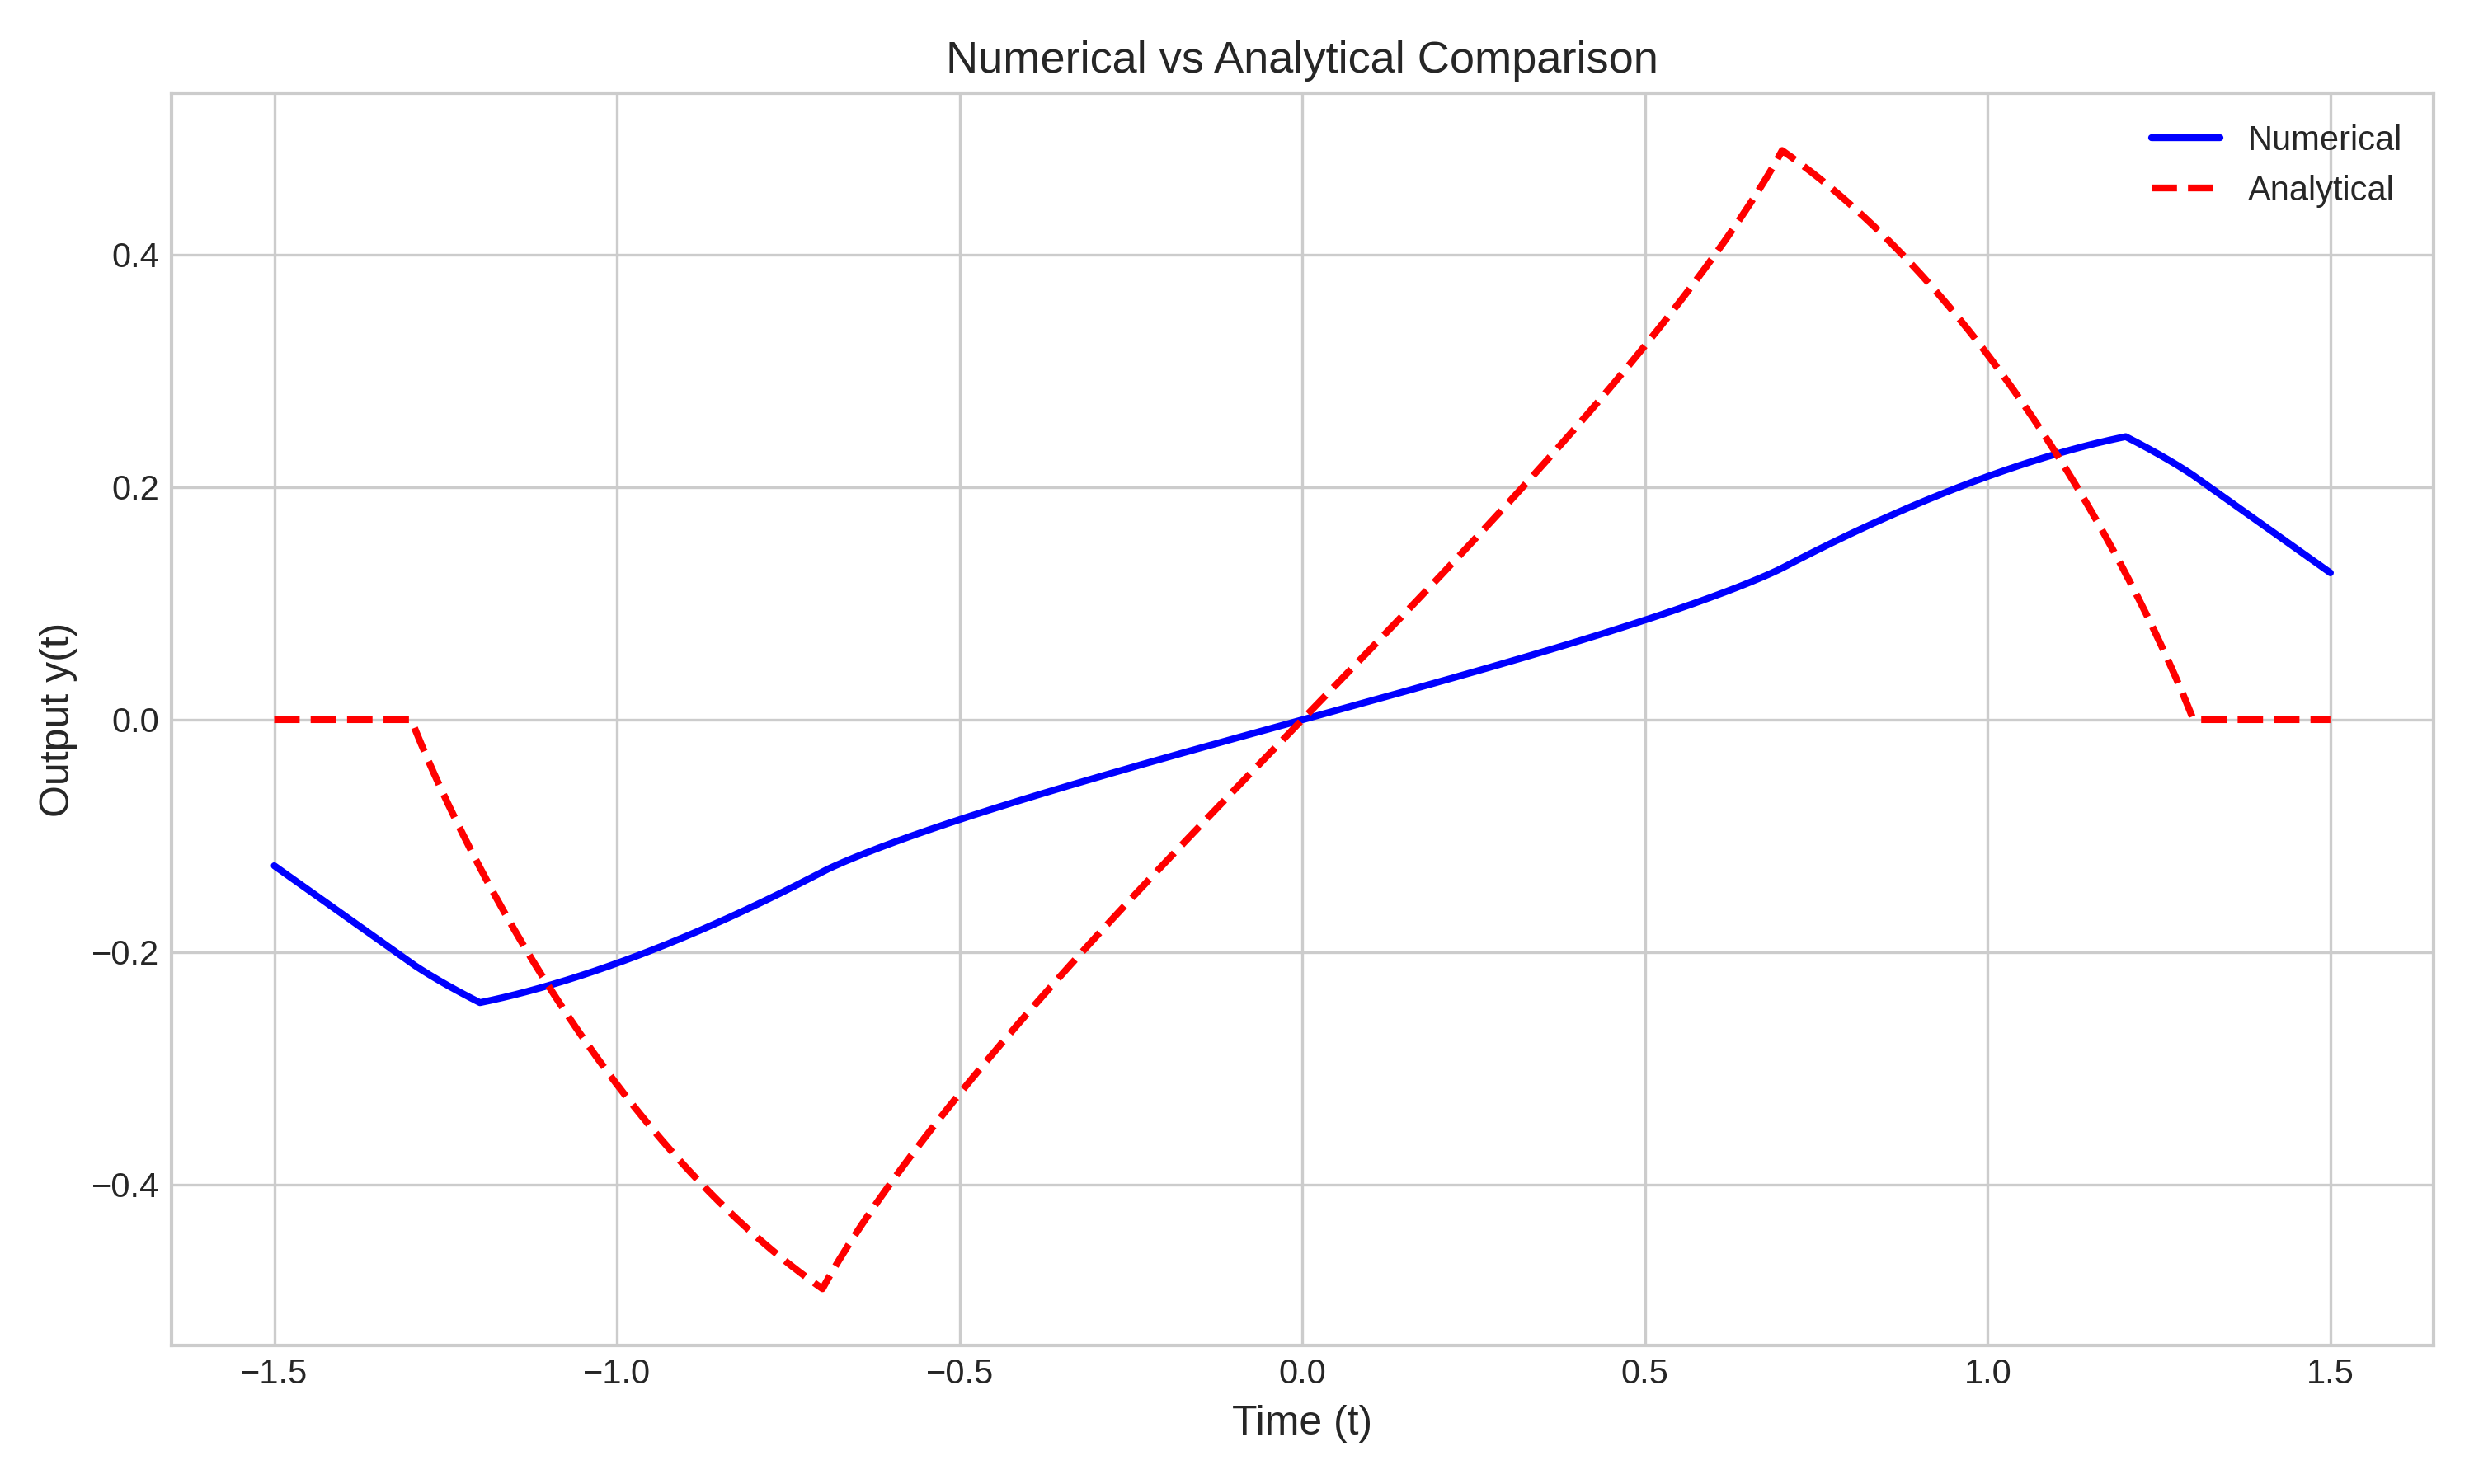
\includegraphics[width=0.85\textwidth]{codes/codes_sin_1_and_arcsin/figures/comparison.png}
    \caption{Numerical vs analytical comparison showing agreement in valid regions}
    \label{fig:comparison}
\end{figure}

Critical findings:
\begin{itemize}
\item Excellent agreement in central region $[-1+T, 1-T]$
\item Boundary discrepancies highlight numerical challenges
\item Analytical solution becomes singular at domain edges
\end{itemize}

\subsection{Conclusion}
This analysis demonstrates that while the arcsin function presents unique challenges for convolution operations, both analytical and numerical methods can provide valuable insights when properly implemented. The key findings include:

\begin{itemize}
\item Linear amplitude scaling with input signal magnitude
\item Direct relationship between kernel width and output amplitude
\item Importance of proper domain handling for arcsin function
\item Necessity of numerical methods for full-domain analysis
\end{itemize}

These results emphasize the importance of understanding domain constraints when working with nonlinear functions in signal processing applications.

\section{Smoothening of curves using the Box Kernel}

When smoothing a signal $f(t)$ using the box kernel $h(t)$, we compute the convolution:

$$
y(t) = (f * h)(t) = \int_{-\infty}^{\infty} f(\tau) h(t - \tau) d\tau
$$

For the rectangular kernel, this simplifies to:

$$
y(t) = \int_{t-T}^{t+T} f(\tau) d\tau
$$

This operation calculates the average value of $f(t)$ over a window of width $2T$ centered at point $t$. 
\newline\newline

This notion of "taking average" effectively "smoothens" or removes the noise of the curve it is convolved with. The box kernel acts as a low-pass filter, averaging out high-frequency noise while preserving the general shape of the signal. The choice of the kernel width $T$ is crucial; a larger $T$ results in greater smoothing but can distort finer features of the signal.

\subsection{Properties of Box Kernel Smoothing}

\subsubsection{Effect of Kernel Width}

The parameter $T$ controls the degree of smoothing:
\begin{itemize}
    \item Small $T$: Preserves more details but retains more noise
    \item Large $T$: Creates smoother curves but may obscure important features
\end{itemize}

\subsubsection{Limitations}

The box kernel produces a less smooth result compared to other kernels like Gaussian because of its abrupt cutoff at the boundaries. This creates a "choppy" appearance, especially in areas with sparse data.

\subsection{Some noisy curves and their convolved output}

Gaussian noise with mean $0$ and standard deviation $0.02$ is added to the original curve and then it is convolved with the box kernel.

\subsubsection{Noisy and Smoothed Sinusoid}
\begin{figure}[!ht]
\centering
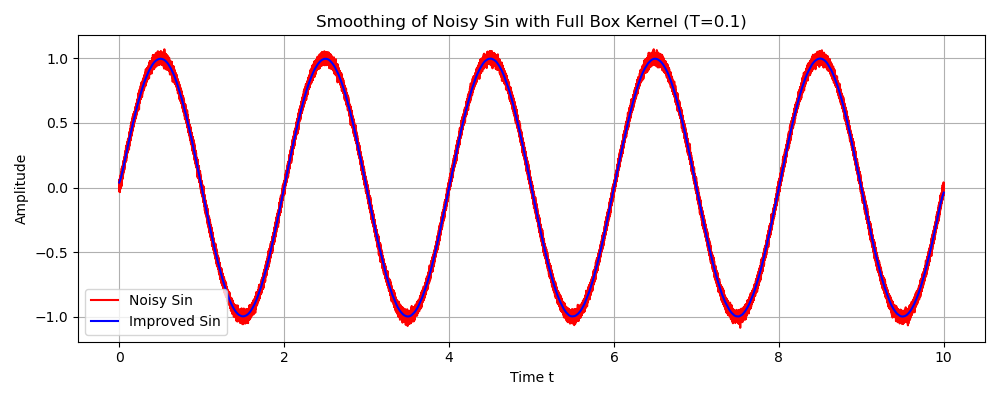
\includegraphics[width=0.8\textwidth]{codes/codes_sin_3_and_smoothening/figs/noisy_sin_plot.png}
\caption{Noisy Sinusoid and Smoothed Sinusoid}
\end{figure}
\FloatBarrier

\subsubsection{Noisy and Smoothed Step Function}
\begin{figure}[!ht]
\centering
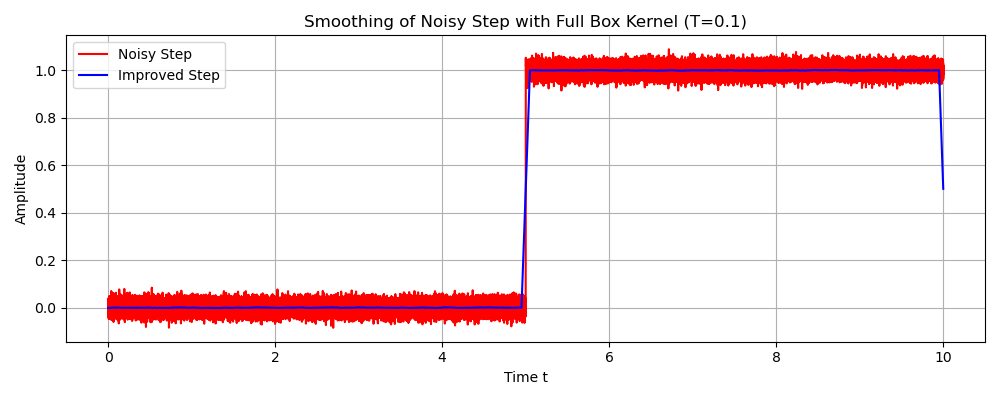
\includegraphics[width=0.8\textwidth]{codes/codes_sin_3_and_smoothening/figs/noisy_step_plot.png}
\caption{Noisy Step and Smoothed Step}
\end{figure}
\FloatBarrier

\subsubsection{Noisy and Smoothed Square Wave}
\begin{figure}[!ht]
\centering
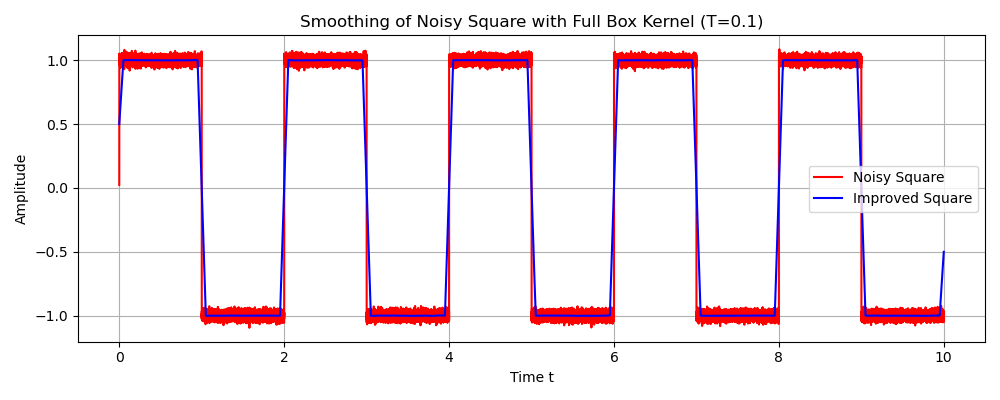
\includegraphics[width=0.8\textwidth]{codes/codes_sin_3_and_smoothening/figs/noisy_square_plot.png}
\caption{Noisy Square Wave and Smoothed Square Wave}
\end{figure}
\FloatBarrier

\subsubsection{Noisy and Smoothed Ramp}
\begin{figure}[!ht]
\centering
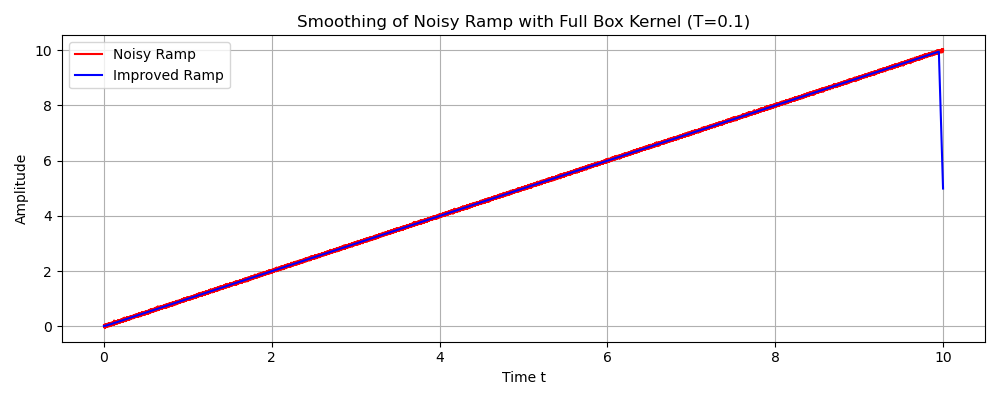
\includegraphics[width=0.8\textwidth]{codes/codes_sin_3_and_smoothening/figs/noisy_ramp_plot.png}
\caption{Noisy Ramp and Smoothed Ramp}
\end{figure}
\FloatBarrier

\subsubsection{Noisy and Smoothed Exponential Decay}
\begin{figure}[!ht]
\centering
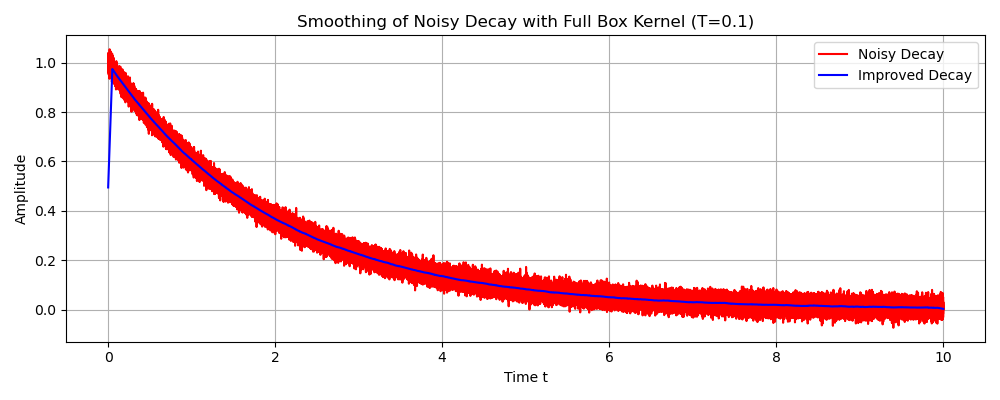
\includegraphics[width=0.8\textwidth]{codes/codes_sin_3_and_smoothening/figs/noisy_decay_plot.png}
\caption{Noisy Exponential Decay and Smoothed Exponential Decay}
\end{figure}
\FloatBarrier

\subsubsection{Noisy and Smoothed Gaussian Curve}
\begin{figure}[!ht]
\centering
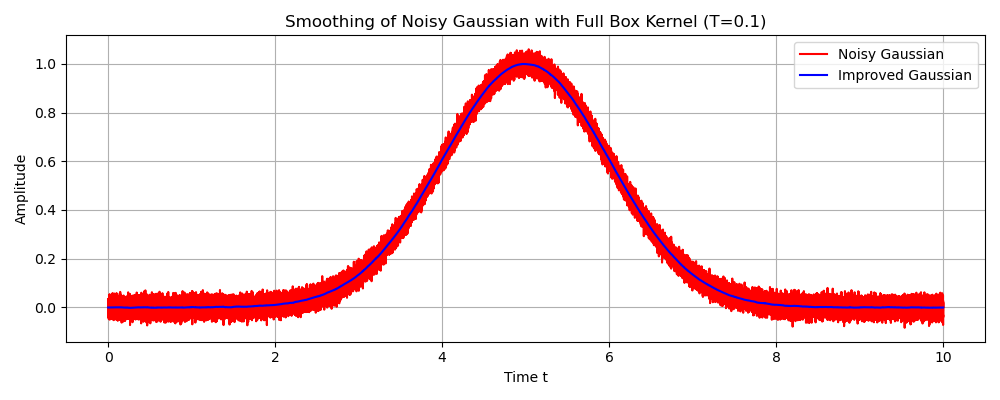
\includegraphics[width=0.8\textwidth]{codes/codes_sin_3_and_smoothening/figs/noisy_gaussian_plot.png}
\caption{Noisy Gaussian and Smoothed Gaussian}
\end{figure}
\FloatBarrier

\subsection{Smoothening out Gibbs phenomena in Fourier Reconstruction using Box Kernel}
Box kernel, in essence, smoothenes out noise. But an relatively interesting usecase would be to reduce the Gibbs Phenomena in the case of Fourier series.
\subsection{Square Wave Fourier Coefficients}
The square wave serves as an excellent example for demonstrating the Gibbs phenomenon. For a square wave alternating between $+1$ and $-1$ with period $2\pi$, the Fourier series is:

\begin{equation}
f(t) = \frac{4}{\pi} \sum_{n=1,3,5,...}^{\infty} \frac{1}{n} \sin(nt)
\end{equation}

\subsection{Convolving the square wave}

By linearity of the convolution operator,
\begin{align}
    (f * h)(t) = \frac{4}{\pi} \sum_{n=1,3,5,...}^{\infty} \left(\frac{2\sin{nT}}{n}\right) \frac{1}{n} \sin(nt) 
\end{align}
This alters the amplitude of the coefficients, which is obviously underisable. If we normalize this convolution amplitude factor, we get:
\begin{align}
    (f * h)(t) = \frac{4}{\pi} \sum_{n=1,3,5,...}^{\infty} \left(\frac{\sin{nT}}{nT}\right) \frac{1}{n} \sin(nt) 
\end{align}


\begin{figure}[!ht]
\centering
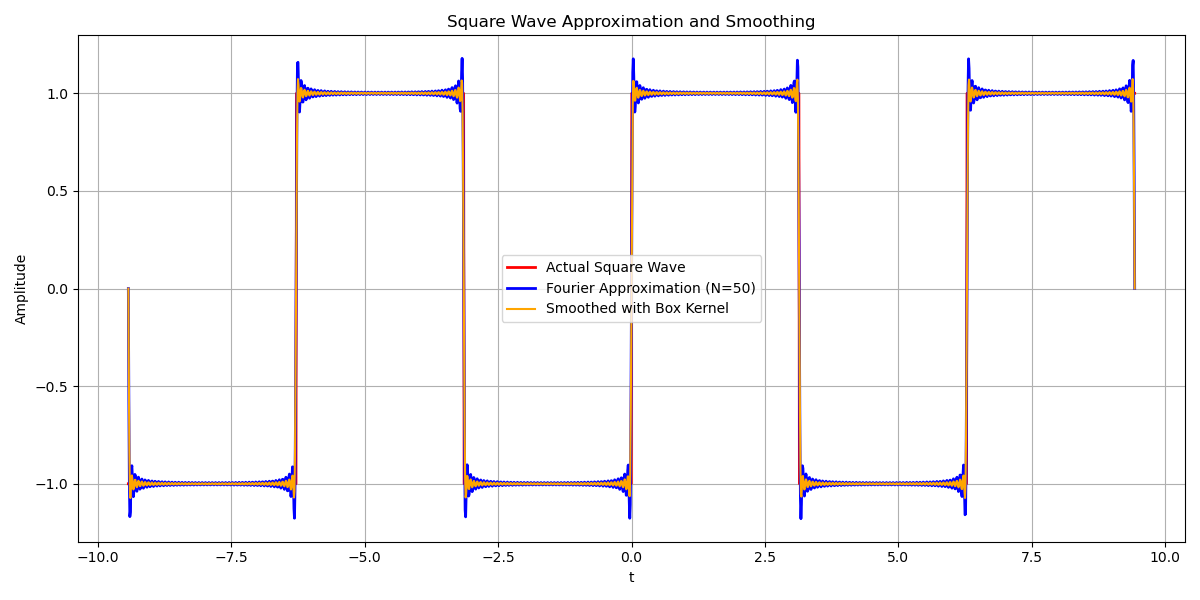
\includegraphics[width=0.8\textwidth]{codes/codes_sin_3_and_smoothening/figs/fourier_box_N50.png}
\caption{Slightly less Gibbs Phenomena in the Fourier Reconstruction at N = 50}
\end{figure}
\FloatBarrier

\begin{figure}[!ht]
\centering
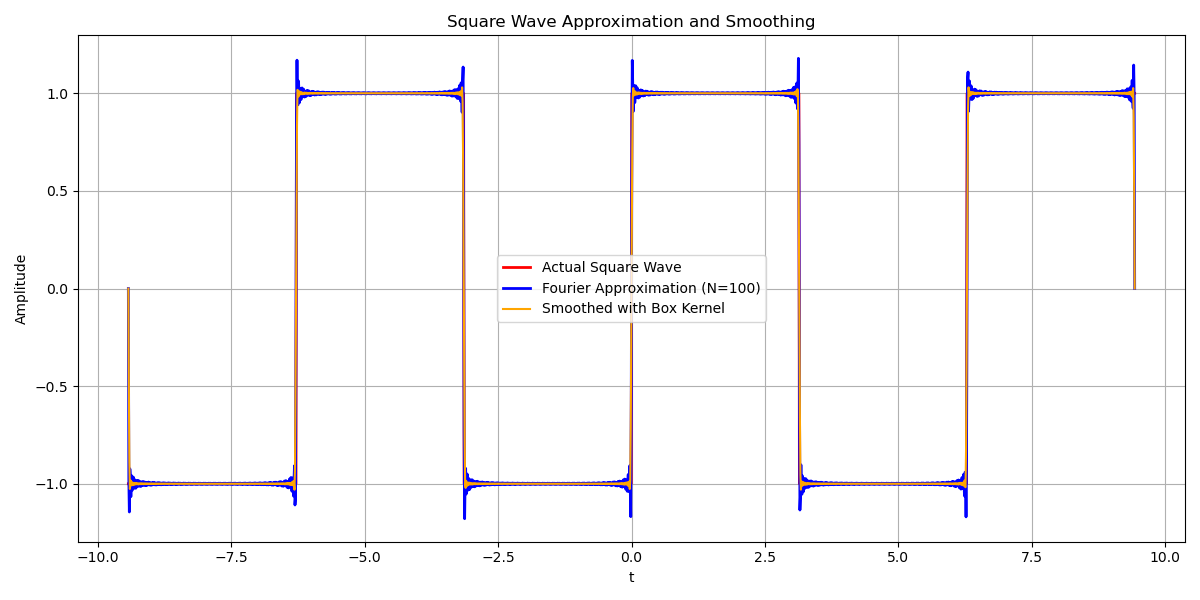
\includegraphics[width=0.8\textwidth]{codes/codes_sin_3_and_smoothening/figs/fourier_box_N100.png}
\caption{Slightly less Gibbs Phenomena in the Fourier Reconstruction at N = 100}
\end{figure}
\FloatBarrier


\end{document}
